\documentclass[11pt]{article}
\usepackage[utf8]{inputenc}
\usepackage{graphicx}
\usepackage{geometry}
\usepackage{parskip}
\usepackage{subcaption}
\usepackage{wrapfig}
\usepackage{acronym}
\usepackage[natbib=true]{biblatex}
\usepackage{amsmath}
\usepackage{dirtytalk}
\usepackage{hyperref}
\usepackage{mathtools}
\usepackage{amsfonts}
\usepackage{csquotes}
\usepackage{pgffor}
\usepackage{algorithm}
\usepackage{algpseudocode}
\usepackage{booktabs}
\usepackage{listings}
\usepackage{bm}
\usepackage{amssymb}
\usepackage{tikz}
\usepackage{lscape}
\usetikzlibrary{shapes,positioning,decorations.pathreplacing}
\addbibresource{literature.bib}
\renewcommand{\baselinestretch}{1.5}
% @formatter:off
\let\oldsection\section
\renewcommand\section{\clearpage\oldsection}
% @formatter:on
\newcounter{savepage}

\lstset{lineskip=-0.7ex,frame=single,breaklines=true}

\DeclarePairedDelimiterX{\infdivx}[2]{(}{)}{%
#1\;\delimsize\|\;#2%
}
\newcommand{\kldiv}{D_{KL}\infdivx}
\DeclarePairedDelimiter{\norm}{\lVert}{\rVert}

\DeclareMathOperator*{\argmin}{arg\,min}
\DeclareMathOperator*{\argmax}{arg\,max}

\makeatletter
\newenvironment{breakablealgorithm}
{% \begin{breakablealgorithm}
\begin{center}
\refstepcounter{algorithm}% New algorithm
    \vspace{1em}
    \hrule height.8pt depth0pt \kern2pt% \@fs@pre for \@fs@ruled
    \renewcommand{\caption}[2][\relax]{% Make a new \caption
    {\raggedright\textbf{\ALG@name~\thealgorithm} ##2\par}%
    \ifx\relax##1\relax % #1 is \relax
    \addcontentsline{loa}{algorithm}{\protect\numberline{\thealgorithm}##2}%
    \else % #1 is not \relax
    \addcontentsline{loa}{algorithm}{\protect\numberline{\thealgorithm}##1}%
    \fi
    \kern2pt\hrule\kern4pt
    }
}{% \end{breakablealgorithm}
\kern2pt\hrule\relax% \@fs@post for \@fs@ruled
\vspace{1em}
\end{center}
}
\makeatother

\begin{document}

\begin{titlepage}
\centering

\includegraphics[width=0.25\textwidth]{rublogo.png}\par
{\scshape\huge\bfseries Semantic Representations in Variational Autoencoders as a Model of the Visual System \par}
{\scshape\large Schriftliche Prüfungsarbeit für die Master-Prüfung des Studiengangs Angewandte Informatik an der Ruhr-Universität Bochum\par}
\vspace{1em}
vorgelegt von\par
\vspace{2em}
Leonard Papenmeier\par 108017257755\par
\vspace{2em}
01.01.1980\par

\vfill
Prof. Dr. Laurenz Wiskott\par
M.Sc. Zahra Fayyaz


\end{titlepage}
\pagenumbering{Roman}

\section*{\centering Abstract}

bla bla bla

\tableofcontents
\newpage
\setcounter{savepage}{\arabic{page}}
\pagenumbering{arabic}


\section{Introduction}\label{sec:introduction}

Research in artificial neural networks has risen in recent years due to their success in a large variety of different tasks.
This increase in research has led to progressively better network architectures, achieving better and better results.
The improvement of network architectures, however, is mainly driven by the question whether a new improvement will lead to better results \citep{lindsay2020convolutional}.

Biological plausibility, an important consideration in the field of computational neuroscience, often is of no interest to researchers aiming at solving a complex problem.
Even though progress in neural network research has become more and more disconnected from the biological example, they are inspired by biology.
Modern neural networks operating on images (mainly \acp{CNN}) indeed share many features with the visual system.

Even though neural networks are trained in a manner largely detached from the way the brain learns and builds memories, it has been shown that image classification networks are related to the visual system, not only areas where this relatedness has been built into the model.

Both, the biological foundation of \acp{CNN} and the more recent insights on their more indirect relatedness to the visual system qualify them as a potentially good model of the visual system.

Unfortunately, the neural networks where this kind of relatedness has been discovered so far are trained in a supervised manner, requiring lots of labeled data.
This kind of learning is disconnected from human perception where often one single example is sufficient when it comes to grouping objects into classes.

The \ac{VAE} is one important representative of a class of models \textit{generative models}.
This class of models allows a different training procedure, still requiring many samples but no labels.
Furthermore, \acp{VAE} build generalizable latent representations of inputs which might be similar to the abstract representation of the brain when perceiving the world.

\acp{VAE}, therefore, could be an important step towards a more realistic model of the visual system.

This thesis aims at answering the question whether \acp{VAE} prove to be a successful model of the visual system.

\section{Theoretical Background}\label{sec:theoretical-background}
The following section presents important theoretical concepts that used in this thesis as well as related work.

\subsection{Human Cognition}\label{subsec:human-brain-structure}

\subsubsection{Cells}

\begin{wrapfigure}[18]{R}{0.3\textwidth}
    \begin{center}
        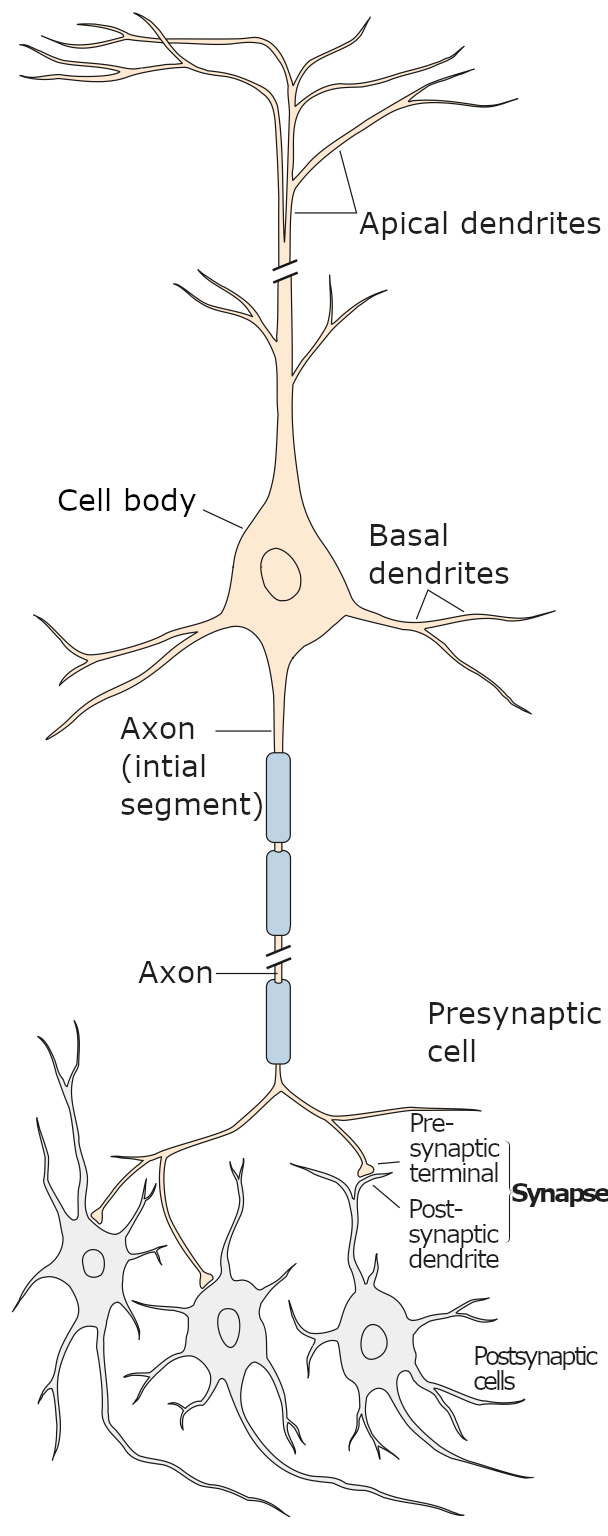
\includegraphics[width=0.28\textwidth]{images/neuron.jpeg}
    \end{center}
    \caption[Neuron structure]{The morphological structure of a neuron, taken from \citet[p. 22]{mack2013principles}}
    \label{fig:neuron_structure}
\end{wrapfigure}

The human nervous systems has two types of cells, \textit{neurons} and \textit{glial cells} or \textit{glia}~\citep[p. 71]{mack2013principles}.
Even though glia occur two to ten times more often in the nervous system than neurons~\citep[p. 24]{mack2013principles}, they - unlike neurons - \say{are not directly involved in electrical signaling}~\citep[p. 26]{mack2013principles} and therefore not further described in the course of this work.

Neurons in different brain regions can take different forms.
However, regardless of their specific configuration, they have four defined regions: \say{(1) the cell body, (2) dendrites, (3) axon, and (4) presynaptic terminals}~\citep[p. 22]{mack2013principles} (see Figure~\ref{fig:neuron_structure}).
The dendrites receive input from other neurons while axons convey electrical signals to other neuron's dendrites.
\textbf{Hier könnte noch deutlich mehr kommen.}

\subsubsection{Human Brain Structure}

The human brain is subdivided into six regions of different forms and functions: the medulla, pons, midbrain, cerebellum, diencephalon, and the cerebral hemispheres~\citep[p. 340]{mack2013principles} (see Figure~\ref{fig:human_brain_divisions}).
Together with the spinal cord, it constitutes the \ac{CNS}~\citep[p. 340]{mack2013principles}.

\begin{figure}
    \centering
    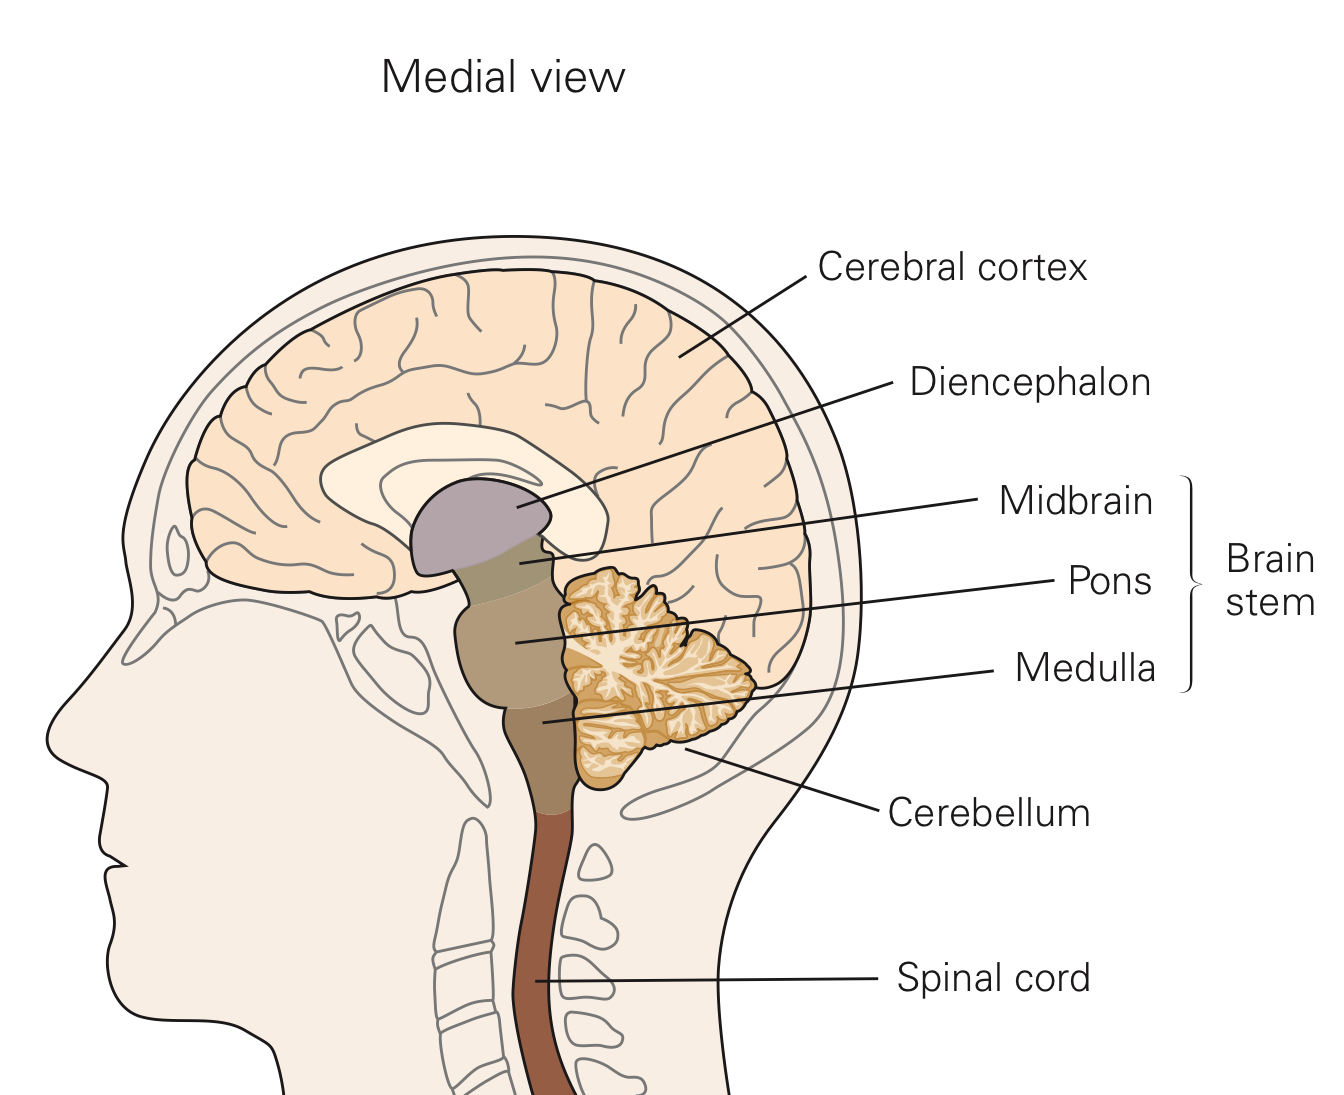
\includegraphics[width=.4\textwidth]{images/brain_regions.jpeg}
    \caption[Divisions of the human brain]{Five divisions of the human brain, the cerebral cortex as part of the cerebral hemispheres, and the spinal cord. Taken from \citet[p. 340]{mack2013principles}.}
    \label{fig:human_brain_divisions}
\end{figure}

Medulla, pons, and midbrain constitute the \textit{brain stem}.
The brain stem recieves input from \say{several specialized senses, such as hearing, balance and taste} and \say{mediates sensation and motor control of head, neck, and face}~\citep[p. 341]{mack2013principles}.
Furthermore, it \say{contains [\ldots] pathways that carry [\ldots] information to other divisions of the \ac{CNS}}~\citep[p. 341]{mack2013principles}.

The \textit{cerebellum} is mostly responsible for motor skills but is also involved in \say{language and other cognitive function}~\citep[p. 341]{mack2013principles}.
Even though containing more neurons than other divisions of the brain, it \say{is well understood because relatively few types of neurons are involved}~\citep[p. 341]{mack2013principles}.

The \textit{diencephalon} contains the \textit{thalamus} and \textit{hypothalamus}.
The thalamus acts as a filter, deciding which information is forwarded to the neocortex~\citep[p. 341]{mack2013principles}.
The hypothalamus plays an important role in controlling body functions such as eating or drinking, but also in initiating behaviors~\citep[p. 341]{mack2013principles}.

The \textit{cerebral hemispheres}~\citep[p. 341]{mack2013principles}, finally, is the brain region most relevant for this thesis.
It can be further subdivided into \textit{cerebral cortex}, \textit{white matter}, \textit{basal ganglia}, \textit{amygdala}, and \textit{hippocampus}~\citep[p. 341]{mack2013principles}.
The latter three are \say{concerned with the expression of emotion [amygdala], [\ldots] memory formation [hippocampus], and [\ldots] control of movement and aspects of motor learning [basal ganglia]}~\citep[p. 342]{mack2013principles}.
The \textit{cerebral cortex}, underlayed by the \textit{white matter}, is the structure of the brain closest to the surface~\citet[p. 341]{mack2013principles}.

The \textit{neocortex} is \say{the region of cerebral cortex nearest the surface of the brain} \citet[p. 345]{mack2013principles}.
It is structured into six layers and columns~\citep[p. 345]{mack2013principles}.
Neurons within a column are assumed to from a \say{local processing network} and are understood as \say{the fundamental computational modules of the neocortex}~\citep[p. 348]{mack2013principles}.
Neurons within the different layers show different kinds of connectivity.
For example, Layer I mainly contains dendrites of cells in deeper layers where as Layers II and III contain \textit{pyramidal neurons} whose axons project onto other neuros~\citep[p. 346]{mack2013principles}.

Furthermore, the neocortex is structured \textit{topographically}, i.e.~neurons within a sensory area (e.g. the skin or retina) are mapped onto the neocortex such that neighboring neurons in the sensory area ultimately map onto neighboring regions in the neocortex~\citep[p. 343]{mack2013principles}.

\subsubsection{Visual Cortex}\label{subsubsec:visual-cortex}

The first cortical region receiving retinal signals is the \acf{V1}~\citep[p. 559]{mack2013principles}.
The \ac{V1} does not receive input directly from the retina, but the signal travels through the \textit{primary visual pathway} that includes the \ac{LGN}~\citep[p. 559]{mack2013principles}.
Two other pathways transport signals from the retina to other brain regions but are not concerned with object recognition but controlling movements and pupillary reflexes~\citep[p. 559]{mack2013principles}.

The \ac{LGN} contains so-called \textit{on-center} and \textit{off-center} cells that respond strongly to stimuli having either a bright center and a dark surrounding or a dark center and a bright surrounding~\citep[pp. 564-566]{mack2013principles}.
Noteworthy, the \ac{LGN} receives strong feedback from \ac{V1}.
However, the function of these feedback connections, outnumbering the number of feedforward neurons from the \ac{LGN} by the factor ten, \say{is largely unknown}~\citep[p. 573]{mack2013principles}.

\begin{figure}
    \centering
    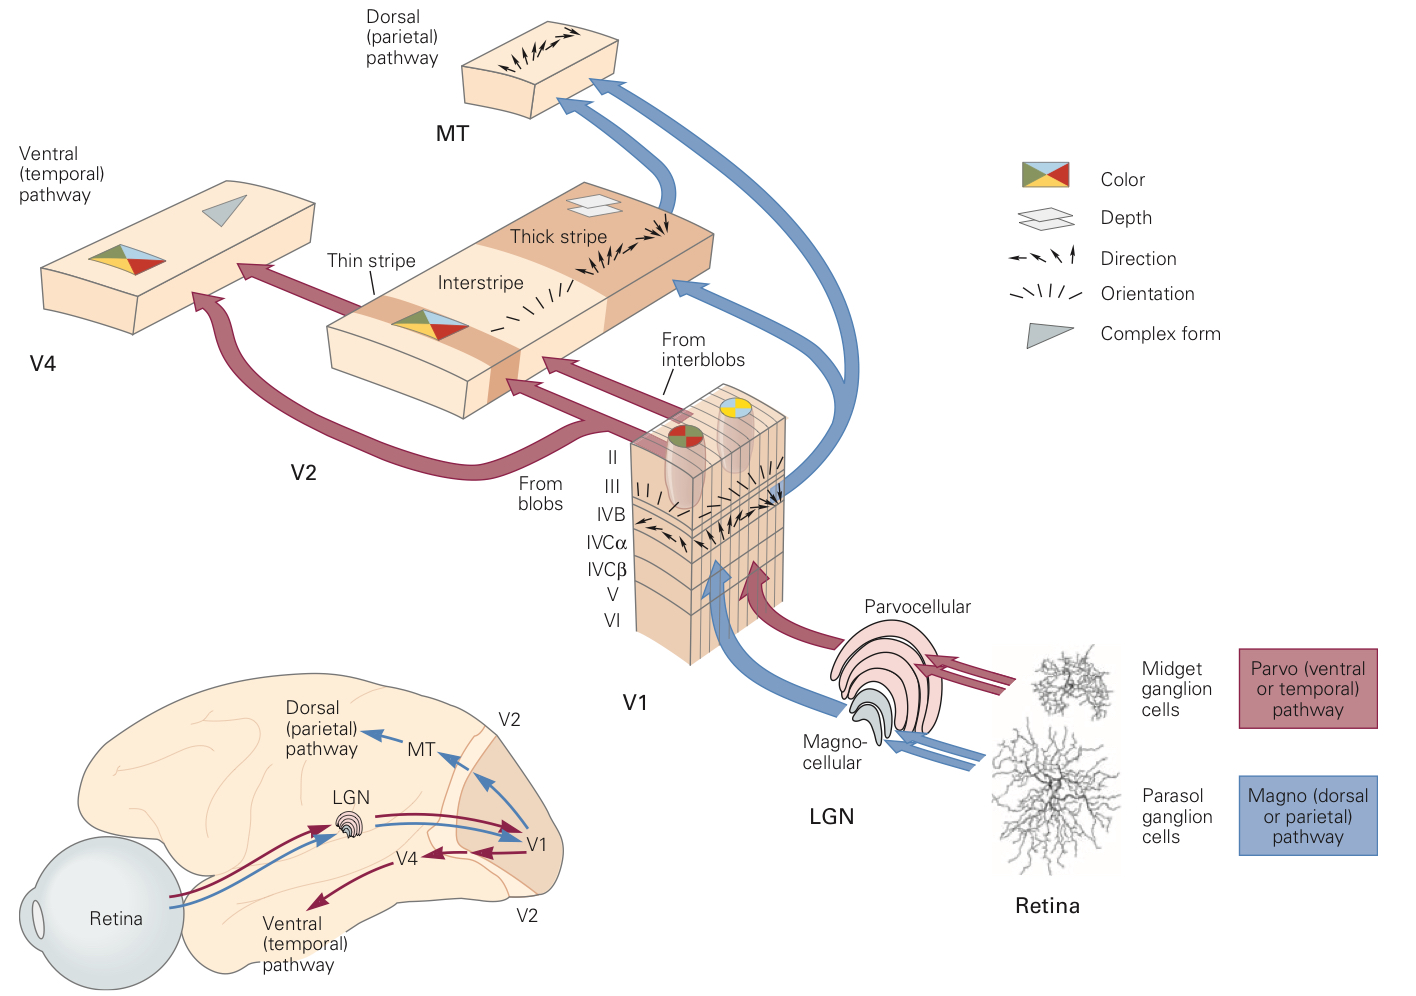
\includegraphics[width=.8\textwidth]{images/ventral_dorsal.jpeg}
    \caption[Ventral and dorsal pathways]{The ventral and dorsal pathways, carrying information from \ac{V1} to other brain regions. Taken from \citet[p. 571]{mack2013principles}}
    \label{fig:ventral_dorsal_pathway}
\end{figure}

From \ac{V1}, information is propagated to other brain regions via the \textit{ventral} and \textit{dorsal} pathways~\citep[pp. 563, 563]{mack2013principles}.
The dorsal pathway is responsible for the pass of information regarding the direction of movements whereas the ventral pathway is more concerned with object recognition~\citep[p. 564]{mack2013principles}.
Figure~\ref{fig:ventral_dorsal_pathway} shows the two pathways and the flow of information.
Importantly, Figure~\ref{fig:ventral_dorsal_pathway} does not show the complete pathways.
From V4, the Ventral pathways has feedback and feedforward connections from and to \ac{TEO}, and from \ac{TEO} it has feedback and feedforward connections from and to \ac{IT}, which, in turn, has feedback connections to \ac{V1}~\citep[p. 563]{mack2013principles}.

The visual cortex is mainly structured in a feed-forward manner.
It is the common view that lower regions in the visual cortex detect lower level features, whereas higher regions detect higher level features~\citep{eickenberg2017seeing}.
The primary visual cortex (\ac{V1}) detects edges~\citep{hubel1962receptive, eickenberg2017seeing}.
The seconday visual cortex (\ac{V2}) does not respond to such easily interpretable shapes~\citep{freeman2013functional}.
Instead, it responds to naturalistic textures that can be expressed in terms of features \ac{V1} is sensitive to~\citep{freeman2013functional}.
The function of V4 is manifold - it \say{respond[s] to more complex geometric shapes, color, and a large number of other
stimulus characteristics}~\citep{eickenberg2017seeing} and it is assumed to perform foreground and background segmentation~\citep{roe2012toward}.
Furthermore, \ac{V4} is assumed to play a role in \say{visual attention}~\citep{roe2012toward}, i.e. to \say{enhance neuronal firing to relevant stimuli in V4 and [to] suppress responses to distractor stimuli}~\citep{roe2012toward}.
It is assumed that this behavior emerges from the top-down connections into \ac{V4}~\citep{roe2012toward}.
\ac{IT}, finally, responds to high level features such as faces and complex objects~\citep{logothetis1995shape, eickenberg2017seeing}.

According to the two-stream hypothesis~\citep{goodale1992separate}, the two pathways are assumed to encode the \textit{what} (dorsal) and \textit{where} (ventral) in a visual scene~\citep[p. 520]{mack2013principles}.
Even though the two pathways can exchange information~\citep[p. 564]{mack2013principles}, they encode two different qualities of a stimulus: the identity and the location.

\subsubsection{Visual Object Perception}\label{subsec:visual-object-perception}

\begin{wrapfigure}[12]{R}{0.3\textwidth}
    \begin{center}
        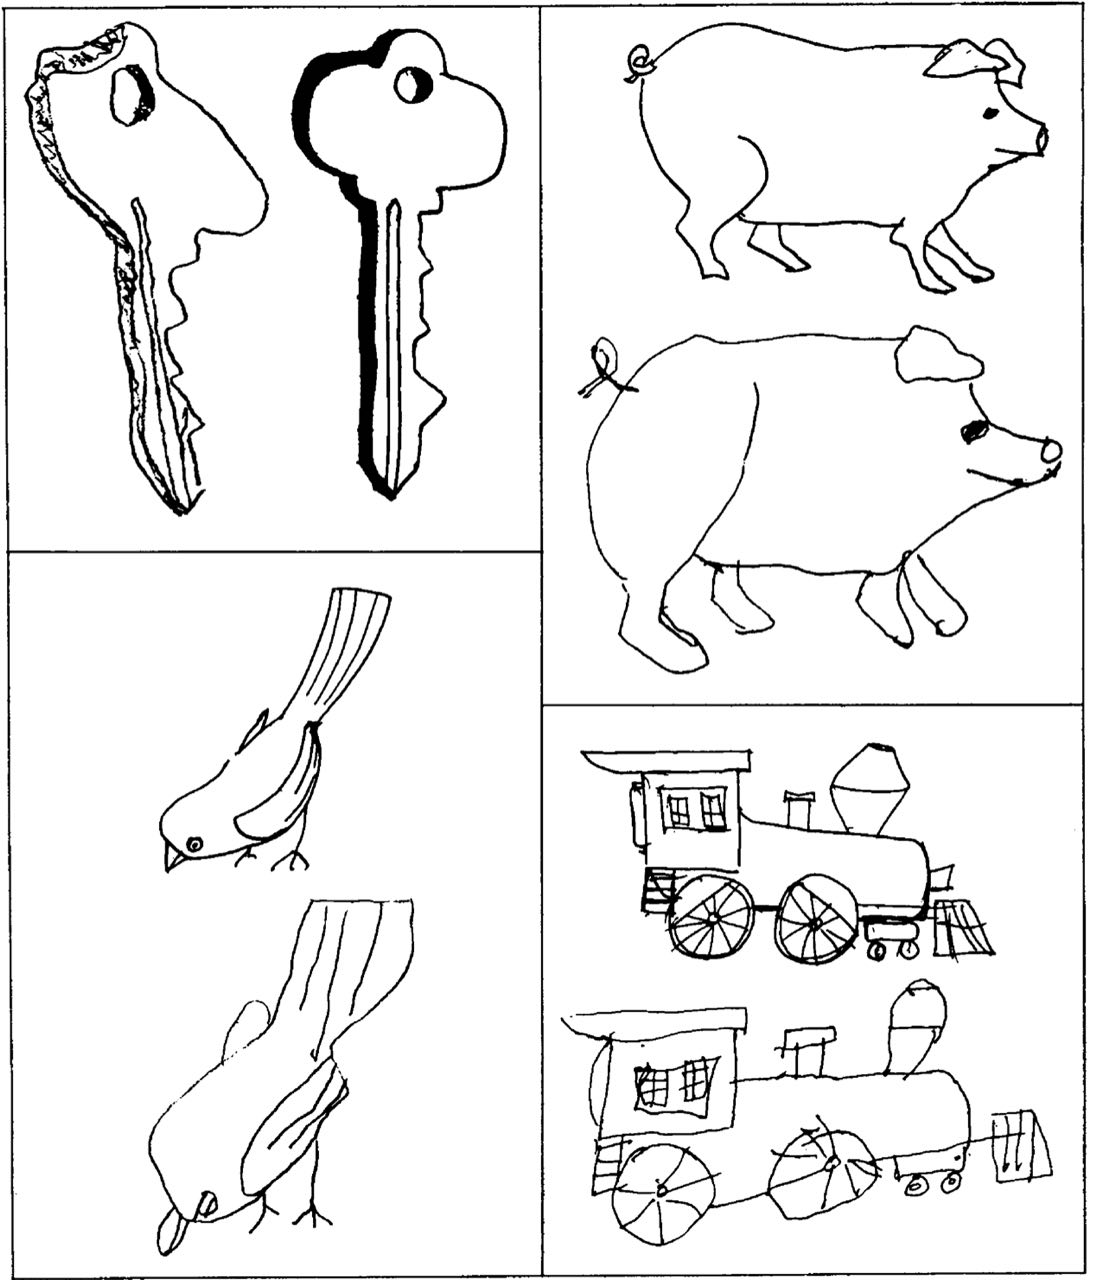
\includegraphics[width=0.28\textwidth]{images/rubens_sketches.jpg}
    \end{center}
    \caption[Copies of line drawings]{\say{Copies of line drawings.} taken from \citet{rubens1971associative}}
    \label{fig:copies_line_drawings}
\end{wrapfigure}
Recognizing an object as what it is is different from the ability of seeing an object or making a copy of it.
\citet{rubens1971associative} report the case of a 47-year old man who, on March 5--1969, \say{was found unconscious with vomitus on his face and bathrobe}.
Only after \say{his breathing became irregularly}, he was taken to a hospital where a low blood pressure was diagnosed.
The man showed an inability to recognize objects and in cases where he was unable to recognize an object, he also could not describe its use.
When given the category of an object, \say{identification improved very slightly}.
He claimed to recognize the item after being told the name.
In such cases, he was able to \say{point out various parts of the previously unrecognized item}.
When shown sketches of items, he was generally unable to recognize the items.
However, he was able to name geometric shapes such as circles or squares present in the sketch.
Even though the man did not recognize the objects, he was able to make copies of them (see Figure~\ref{fig:copies_line_drawings}).
\citet{rubens1971associative} report, that the Patient \say{was unable to identify any [items] before copying}.
However, he was able to contain some of the objects categories after copying them.

The example presented above shows that the ability to reproduce an object is different from the ability to \textit{perceive} it.

For monkeys, the \ac{IT} is assumed to be the brain region being crucial for object perception~\citep[pp. 1070, 1071]{squire2012fundamental}.
Bilateral lesions of the \ac{IT} in monkeys affect their ability to \say{distinguish between different visual patterns or objects, and in retaining previously acquired visual discriminations}~\citep[p. 1070]{squire2012fundamental}.
They are no longer able to generalize from tasks learned in one half of the visual space to the other half, presumably because the invariance of representations is lost~\citep[p. 1070]{squire2012fundamental}.
\citet[p. 1071]{squire2012fundamental} explicitly point out \say{the crucial role of the inferior temporal cortex during object perception and recognition}.

\subsubsection{Sparse Representations}\label{subsubsec:sparse_representations}

The brain uses sparsesness to represent information~\citep{yoshida2020natural} (\textbf{More references?}).
When shown natural images, between 1.8\% and 3.0\% (with $p < 0.01$) of mice \ac{V1} neurons are active across planes~\citep{yoshida2020natural}.
The overlap of responsive neurons for different images is quite small.
Between 4.8\% and 6.0\% of neurons overlap for different natural images.

\textbf{DRAFT!} More could come here

\subsection{Models of the Visual System}

\subsubsection{Simple and Complex Cells in \ac{V1}}\label{subsubseq:simple_complex_cells}

\citet{hubel1962receptive} distinguish two main types of cells in the primary visual cortex: simple and complex cells.
Both cell types are orientation sensitive, i.e. different cells are tuned towards different orientations of stripes in a stimulus.
Other than simple cells, complex cells are more invariant towards the stripe's location (but not it's orientation) in the receptive field.
Complex cells are assumed to receive input from simple cells~\citep{hubel1962receptive}.

Based on this assumption, complex cells can be modelled by receiving input from many simple cells, tuned towards a specific orientation but not translation.
If any of the afferent simple cells fire, the complex cells fires as well, leading to an translation invariant behavior~\citep{hubel1962receptive}.

It can be shown that a two-dimensional Gabor wavelet is a very good stimulus for a simple cell in \ac{V1} in terms of neuron excitation~\citep{jones1987evaluation}.

\subsubsection{Neocognitron}

The Neocognitron~\citep{fukushima1980neocognitron} is a model of object perception.
It aims at modelling the ventral stream based on the findings of \citet{hubel1962receptive}.
It is a neural network, consisting of models of simple (\say{S-cells}) and complex (\say{C-cells}) cells, arranged alternating in multiple layers.
It can be trained in an unsupervised manner by reinforcing connections leading to high cells activations in the next layer and has shown to be effective in pattern recognition.

\subsubsection{\acp{CNN}}
\acp{CNN}~\citep{lecun1989backpropagation} can be understood as a successor of the Neocognitron~\citep{lindsay2020convolutional} and is a network type commonly used on image data~\citep[p. 326]{Goodfellow-et-al-2016}.
The constituent of \acp{CNN} giving it it's name are the convolutional layers that act as a pattern detector, similar to the S-cells in the Neocognitron~\citep{lindsay2020convolutional}.
In addition, after an activation layer, many neural networks subsequently perform an operation called (max-)pooling~\citep[pp. 326, 339]{Goodfellow-et-al-2016}.
The pooling operation introduces invariance to the network, similar to C-cells~\citep{lindsay2020convolutional}.

\paragraph{Convolution}

Assume $I$ is a two-dimensional grayscale image and $K$ is a xconvolutional kernel.
Then, the convolution operation can be written as~\citep[p. 327]{Goodfellow-et-al-2016}:
\begin{align}
    S(i, j)=(I * K)(i, j)=\sum_{m=-\infty}^{\infty} \sum_{n=-\infty}^{\infty} I(m, n) K(i-m, j-n) \label{eq:conv}
\end{align}

The result of the convolution is $S$, a \textit{feature map}.

The kernel usually is implemented as a two-dimensional array~\citep[p. 327]{Goodfellow-et-al-2016}.
Values outside of this array, as they are assumed in the summation in Equation~\ref{eq:conv}, are assumed to be zero.
These values then do not contribute to the sum and the convolution effectively only has to use a finite number of summations.
In case of a $3\times 3$ kernel, Equation~\ref{eq:conv} boils down to:
\begin{align}
    S(i, j)=(I * K)(i, j)=\sum_{m=i-1}^{i+1} \sum_{n=j-1}^{j+1} I(m, n) K(i-m, j-n) \label{eq:conv_boiled_down}
\end{align}
assuming that indexing starts at zero for the image and at minus one for the kernel.

The output of a convolution is maximum in image areas where the image contains a flipped version of the kernel.
This is because the sums in Equation~\ref{eq:conv_boiled_down} go from low to high indices for the image but from high to low indices for the kernel.

Other than the cross-correlation\footnote{The cross-correlation is defined as $S(i, j)=(I * K)(i, j)=\sum_{m=-\infty}^{\infty} \sum_{n=-\infty}^{\infty} I(i+m, j+n) K(m, n)$~\citep[p. 329]{Goodfellow-et-al-2016}.}, the convolution is commutative.
However, this property is not important in practice and \say{many neural network libraries implement [...] the cross-correlation [instead]}~\citep[p. 329]{Goodfellow-et-al-2016}.

\subparagraph{Padding}
The convolution operations applies the kernel at all image locations.
At border pixels, however, this leads to a problem because the sum in Equation~\ref{eq:conv_boiled_down} also considers image pixels with an index smaller than $i$ or $j$.
There are multiple options to deal with this problem.

One option is to not pad the image at all and to start and end the convolution at indices such that the sum in Equation~\ref{eq:conv_boiled_down} never \say{touches} invalid image \textbf{indices}~\citep[p. 350]{Goodfellow-et-al-2016}.
This, however, leads to smaller resulting feature maps as the border pixels are not considered.
This can be problematic in cases where the network has to be very deep as this happens on all convolutional layers.
Also, the network is not as able to make sense of border pixels as for inner pixels.

Another option is \textit{zero-padding}~\citep[p. 350]{Goodfellow-et-al-2016}, i.e. to assume values outside the image to be zero.
Here, the feature map is of the same size (assuming no strided convolution) as the input.
However, the network still handles border pixels differently than inner pixels as the feature map values for border pixels tend to be smaller due to the multiplication with zero in Equation~\ref{eq:conv_boiled_down}.

Other padding techniques mirror the image at the borders or assume that all pixel values outside the image are the same as at the borders~\footnote{\href{https://www.tensorflow.org/api\_docs/python/tf/pad}{https://www.tensorflow.org/api\_docs/python/tf/pad}, last access: 2020/06/18}.

\paragraph{Max-Pooling}
Similar to the convolution, pooling operations use a sliding window over the feature maps, often with an offset (\textit{stride}) such that the sliding window sees every pixel only once.
A strided max-pooling has multiple effects.

First, it leads to a downsampling of the image.
This is a useful property as it allows to use more convolutional kernels in higher layers without exceeding a system's memory\footnote{Of course, the convolutional kernels itself are almost certainly unproblematic as they are very small. Each convolution, however, produces another memory-consuming feature map.}.

Not less importantly, max-pooling introduces invariance to small translations to the network~\citep[p. 342]{Goodfellow-et-al-2016}.

In cases where this translation invariance is not desired\footnote{This is often the case for generative models.} but the image should be down-sampled, the max-pooling layer can be omitted and a strided convolution can be used instead~\citep[p. 337]{Goodfellow-et-al-2016}.

\paragraph{\acp{CNN} as Models of the Visual System}
As discussed earlier, \acp{CNN} by design share some features with the visual system, namely the convolution as a model of S-cells and max-pooling as a model of C-cells.
Surprisingly, some \acp{CNN} are also related in ways not explicitly built into this model.

AlexNet~\citep{krizhevsky2012imagenet} is a deep \ac{CNN} trained on image classification.
\citet{krizhevsky2012imagenet} have shown that this network learns Gabor wavelets in the kernels of the first layer.
Importantly, a Gabor-like kernel is most excited by a Gabor wavelet itself, which is the optimal stimulus for cells in \ac{V1} (see Section~\ref{subsubseq:simple_complex_cells} and \citet{jones1987evaluation}).

Furthermore, \citet{khaligh2014deep} have shown that \acp{CNN} trained in a supervised manner show similar \acp{RDM} as the human \ac{IT}.
A \ac{RDM} is a matrix encoding the correlation of activity patterns for a given model.
Rows and columns refer to different input stimuli.
A cell in a \ac{RDM} then contains the correlation of the activity patterns for the given input stimuli and the given model.
\acp{RDM}, therefore, are symmetric.

\citet{eickenberg2017seeing} explicitly discuss \acp{CNN} as models of the visual system.
Their findings show that \say{early visual areas are better described by lower level convolutional net layers and later visual areas by higher level net layers, exhibiting a progression across ventral and dorsal streams}~\citep{eickenberg2017seeing, wen2018neural}.


The similarity of the \acp{RDM} is evidence of that supervised \acp{CNN} and the human \ac{IT} have a similar high-level encoding of information.

\citet{khaligh2014deep} also show that this is not true for a variety of unsupervised models.
The unsupervised models under investigation, however, are only losely related to \acp{VAE}.
The question whether \acp{VAE} show similar \acp{RDM} as the human \ac{IT}, therefore, remains.

It has been shown that \acp{VAE}, trained in a self-supervised manner, partially learn Gabor wavelets when trained to predict the next image in a sequence of images~\citep{palm2012prediction}.

\subsection{Types of Learning}\label{subsec:types-of-learning}

In machine learning, one often distinguishes between the three fundamentally different types of learning that are roughly described in the following.

\paragraph{Supervised Learning}
Algorithms employing supervised learning learn to predict the label for images representative for the training set.
Datasets for this type of learning usually consist of sets of images (or \textit{samples}) $\bm{x}_i$ and \textit{labels} $y_i$ where the label describes what is present in the image, e.g. \say{dog} or \say{cat}.
An example for supervised learning is \textit{object detection} where one is interested in predicting what is present in an image or a sequence of images.

It is not always the case that a pre-defined and discrete set of samples and labels exist.

In \textit{active learning} the learning algorithm has no beforehand-dataset but has to query labels for self-chosen datapoints in the sample space.
In this setting, the learning algorithm chooses itself what points to use for learning.
Active learning often is used in the context of \textit{hyperparameter optimization}.
Most learning algorithms have a set of parameters that are not learned by the algorithm itself, but are set by the user, e.g. the learning rate or the number of neurons in one layer.
Hyperparameter optimization aims at finding the best combination of these parameters in terms of learning algorithm performance.
For a classifier, the performance can be expressed as the accuracy, i.e. the fraction of correct predictions.
In this context, one datapoint is a specific hyperparameter combination and the corresponding label is the accuracy of the classifier trained with these hyperparameters.
Since the space of possible datapoints is large, possibly infinitely large for continuous values such as the learning rate, and one function evaluation is computationally expensive, it is usually not possibly to simply visit all datapoints.
Besides others, Bayesian Optimization~\citep{mockus1978application} is one technique to approach this problem.

In the introductory example of this paragraph, the dataset was present beforehand.
In such settings, the learning algorithm learns the mapping function and does not update it once the learning is finished.
Contrary to this is \textit{online learning} where the mapping function is updated during the lifetime of a system.
An example for this are recommender systems, e.g.~for streaming services.
Users get recommendations while they are using the service but also provide new labels for the algorithm as they rate watched movies.

\textit{Self-supervised learning} can be seen as a special case of supervised learning where the learning algorithm creates the labels itself.
An example for this type of learning is the prediction of the next frame in a video \textbf{REF}.
The dataset has no labels as in the introductory example of this paragraph.
However, given a sequence $\bm{x}_{i,1},\bm{x}_{i,2},\dots,\bm{x}_{i,n}$ of images in a video, the sample at time $t$ can be considered as the supervised training set $((\bm{x}_{i,1},\bm{x}_{i,2},\dots,\bm{x}_{i,t}),\bm{x}_{i,t+1}), \quad 1\leq t\leq n-1$.
Self-supervised learning can also be seen as a subtype of unsupervised learning, however algorithms employing this approach usually use classical supervised learning techniques.
Another example for self-supervised learning are word embeddings \textbf{REF}.

\paragraph{Unsupervised Learning}
\begin{wrapfigure}[11]{R}{0.5\textwidth}
    \centering
    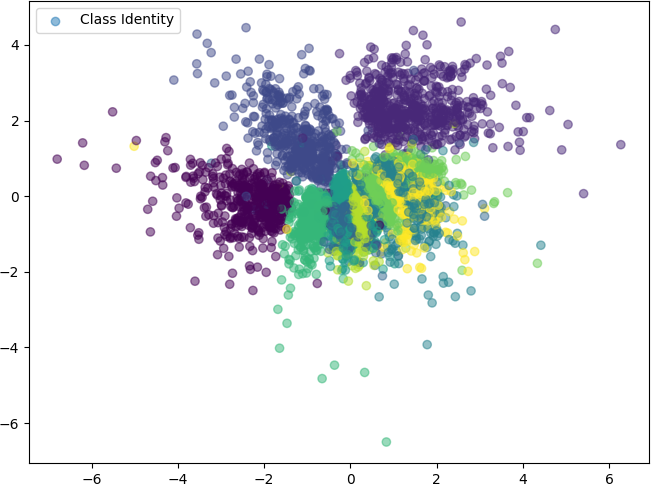
\includegraphics[width=.48\textwidth]{images/latent_spaces/mnist/vae/embeddings_mu_6.png}
    \caption[Clusters of data points]{Data points colored by their corresponding class building clusters.}
    \label{fig:clustering_example}
\end{wrapfigure}
Just like in self-supervised learning, unsupervised learning works with unlabeled data, i.e.~the dataset only consists of samples $\bm{x}_i$.
A typical example for unsupervised learning is clustering, an approach that can be used if the datapoints can be compared in terms of a distance measure.
Consider Figure~\ref{fig:clustering_example}.
Each data point belongs to one class, visualized by the color of the point.

Cluster algorithms often are employed in cases where the class identity of data points is unknown, i.e.~they aim at finding the labeling function by identifying clusters of data points.
Figure~\ref{fig:clustering_example} shows an example where this can be feasible because adjacent data points tend to have the same class.

\paragraph{Reinforcement Learning}
Reinforcement learning is a very different paradigm compared to supervised and unsupervised learning.
Here, the aim to is train an \textit{agent} to show some meaningful behavior, e.g.~to play a computer game.
Reinforcement learning algorithms achieve this by letting the agent explore the action space\footnote{In the case of a computer game, this would mean to carry out different moves.}.
If the outcome of an action is good, the agent is getting rewarded.
The agent, in turn, aims at maximizing its reward. \textbf{REFERENCES FOR THIS PARAGRAPH}

\subsection{Generative Methods}\label{subsec:generative-methods}

Section~\ref{subsec:types-of-learning} used the example of a \say{cat-and-dog-classifier} to introduce supervised learning.
Such as classifier also is an example of a \textit{discriminative model} because it \say{model[s] the posterior probabilities directly}~\citep[p. 43]{bishop2006pattern}.
Therefore, a discriminative model, for example, does not allow to predict the probability density of a data point in the feature space~\citep[pp. 43,44]{bishop2006pattern}.

\textit{Generative methods} model both, the input and the output probabilities.
This allows to sample from the input space, for example to generate new data points~\citep[p. 43]{bishop2006pattern}.

The following sections describe different generative methods.

\subsubsection{\acfp{GAN}}\label{subsubsec:gans}

The idea behind \acp{GAN}~\citep{goodfellow2014gans} is to use two networks, one \textit{generator network} $G$ to approximate the data distribution, and one \textit{discriminator network} $D \mapsto [0, 1]$ to discriminate between true data points and data points generated by the generator network.
This can be formalized as~\citep{goodfellow2014gans}:
\begin{align}
    V(D, G)=\mathbb{E}_{\bm{x} \sim p_{\text{data}}(\bm{x})}[\log D(\bm{x})]+\mathbb{E}_{\bm{z} \sim p_{\bm{z}}(\bm{z})}[\log (1-D(G(\bm{z})))]
\end{align}
where $\bm{z}$ is random noise.

One usually is interested in the generator.
It can be found by~\citep{goodfellow2014gans}:
\begin{align}
    G^* = \argmin_G \max_{D} V(D, G) \label{eq:gan_objective}
\end{align}

Consider Equation~\ref{eq:gan_objective}.

The discriminator $D$ is trained towards maximizing $V(D, G)$.
A perfect discriminator achieves this by labeling all true samples $\bm{x} \sim p_{\text{data}}$ with 1 and all generated samples $G(\bm{z}), \bm{z}\sim p_{\bm{z}}$ with 0.
This would result in a value of $V(D, G) = 0$, which is the maximum.

The generator $G$ is trained towards minimizing $V(D, G)$.
As the discriminator output is the only variable term in $V(D, G)$, this can only be achieved by misleading the discriminator such that it makes a larger error.
The generator can achieve this by reproducing the data distribution $p_{\text{data}}$, then the discriminator would no longer be able to distinguish generated from true samples as they come from the same distribution.
Reproducing the data distribution is what is desired in generative methods (see introduction of Section~\ref{subsec:generative-methods}).

\begin{figure}
    \centering
    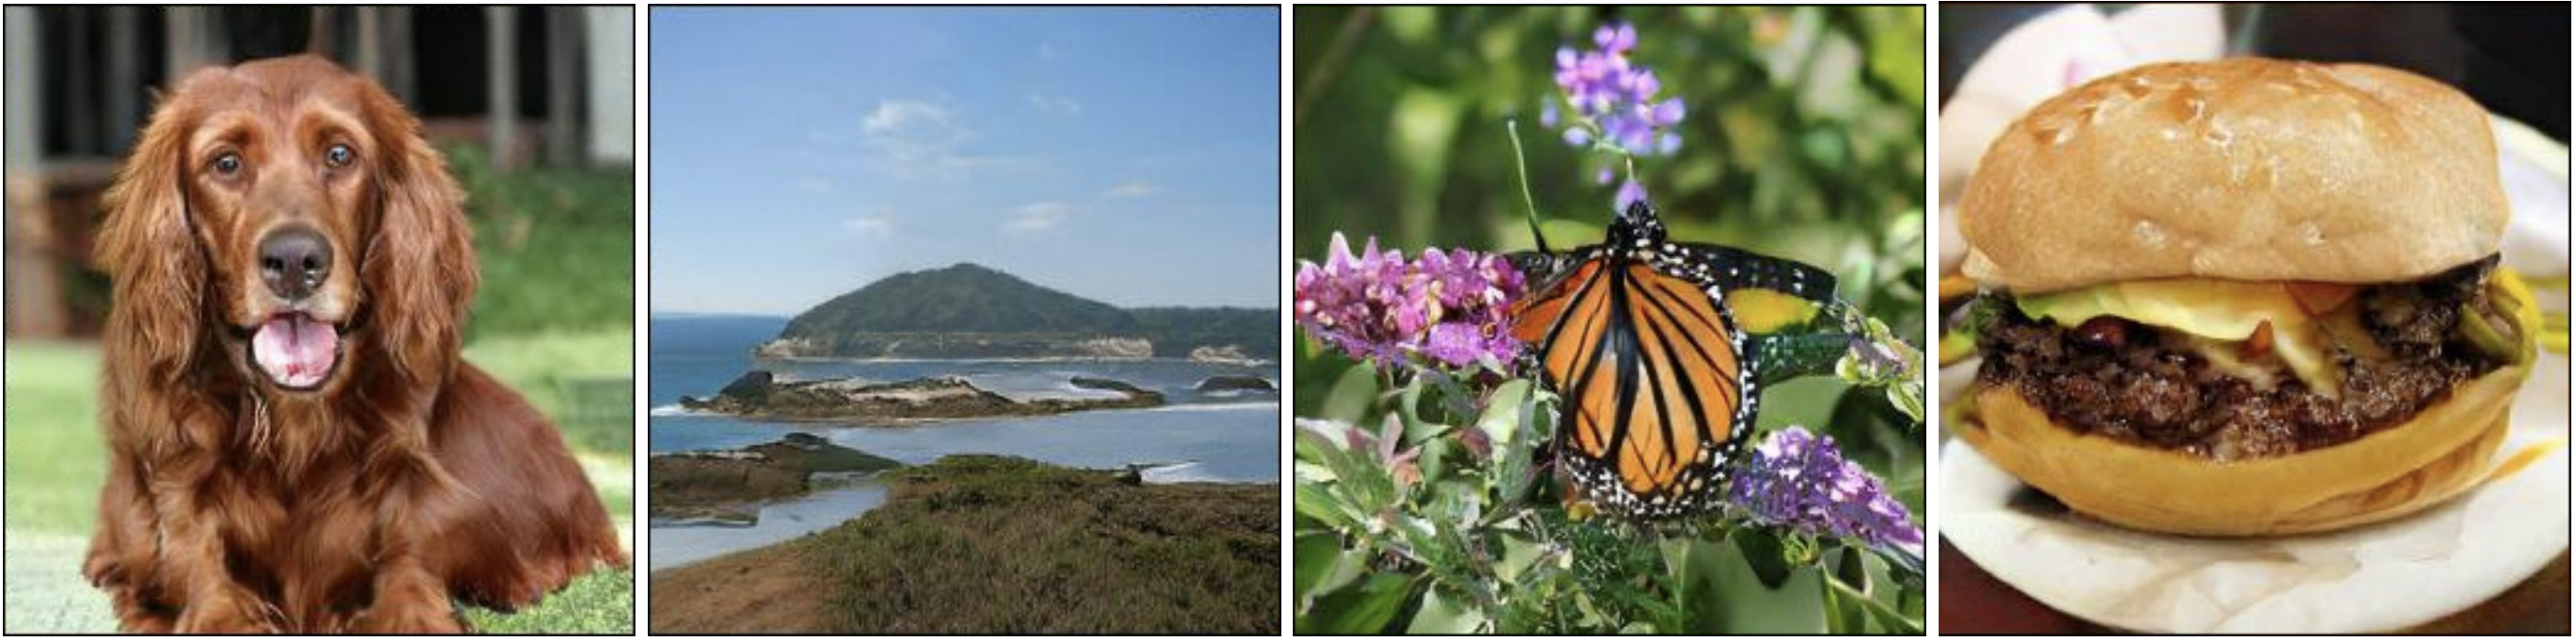
\includegraphics[width=\textwidth]{images/gan_samples.png}
    \caption[\ac{GAN}-generated samples]{\ac{GAN}-generated samples, taken from \citet{brock2018large}.}
    \label{fig:gan_samples}
\end{figure}

Recent improvements on \acp{GAN} have led to synthesis of highly natural images as shown in Figure~\ref{fig:gan_samples}.

\paragraph{Problems with \acp{GAN}}
\textbf{DRAFT}

\subsubsection{Variational Autoencoders}\label{subsec:variational-autoencoders}

Since \acfp{VAE} are a specialization of the autoencoder, the traditional autoencoder is introduced first.

\paragraph{Autoencoders}

Autoencoders are neural networks trained to reconstruct their input~\citep[p. 499]{Goodfellow-et-al-2016}.
For autoencoders, it is common to speak of an \textit{encoder}-part and a \textit{decoder}-part.
The encoder $f: \mathbb{R}^n \mapsto \mathbb{R}^m$ transforms an input $\bm{x}$ to a hidden representation $\bm{r} = f(\bm{x})$.
Usually $m < n$, i.e.\ the encoder transforms the input to a lower-dimensional representation.
This can be beneficial for dimensionality reduction or feature learning~\citep[p. 499]{Goodfellow-et-al-2016}.
The decoder $g: \mathbb{R}^m \mapsto \mathbb{R}^n$ transforms the hidden representation back into the original feature space.
Usually, one wants the reconstruction $\tilde{x}$ to be close to the original feature $x$ ($\tilde{x} \approx x$).
In order to achieve this, the autoencoder is usually trained by minimizing $\mathcal{L}(\bm{x}, g(f(\bm{x})))$ with
\begin{align}
    \mathcal{L}: \mathbb{R}^n \times \mathbb{R}^n \mapsto \mathbb{R}
\end{align}
One common choice for $\mathcal{L}$ is the \ac{MSE} which is defined as
\begin{align}
    \mathcal{L}(\bm{x}, \bm{y}) = \frac{1}{n}\sum (\bm{x}_i - \bm{y}_i)^2 \label{eq:mse}
\end{align}~\citep[p. 106]{Goodfellow-et-al-2016}.
Note that for linear activations in the autoencoder, the space spanned by the first $m$ principal components is the optimal solution for equation~\ref{eq:mse}~\citep{chicco2014deep}.

\paragraph{Variational Autoencoders}

Autoencoders transform an input image to a \textit{hidden representation} $f(\bm{x})$.
However, the distribution over $f(\bm{x})$ is generally unknown.
Let $\bm{z} = f(\bm{x})$.
Assume $\bm{\tilde{z}} = \bm{z} + \bm{\epsilon}$ is a slightly perturbed version of $\bm{z}$, created by adding a small amount of noise $\bm{\epsilon}$.
Even though $\bm{\tilde{z}} \approx \bm{z}$, for example in terms of equation~\ref{eq:mse}, the result after decoding can be very different, i.e. $g(\bm{\tilde{z}}) \not\approx g(\bm{z})$ (again, in terms of equation~\ref{eq:mse}).
This is because the distribution $P(\bm{z})$ can take any arbitrary form.
Values of $\bm{z}$ that are one close to another\footnote{For example in terms of Euclidean distance} can be likely for very different values of $\bm{x}$.

To \textit{generate} new images it would be advantageous to enforce $P(\bm{z})$ to follow a certain distribution.
A common choice is a multivariate normal distribution without covariances~\citep[pp. 24, 25]{kingma2019introduction}.
\acp{VAE} enforce a certain (usually Gaussian) distribution over $\bm{z}$.

\acp{VAE} are trained to generate samples that are likely to occur in the training set.
Therefore, they aim to maximize $\log p(\bm{x})$\footnote{Note that $\max \log  p(\bm{x}) \equiv \max  p(\bm{x})$.}~\citep[p. 18]{kingma2019introduction}.
Assuming a latent distribution $p(\bm{z})$ over $\bm{z}$, we can write $p(\bm{x})$ as the marginal distribution
\begin{align}
    p(\bm{x}) &= \int p(\bm{x}, \bm{z})d\bm{z} \label{eq:vae_x1}\\
    &= \int p(\bm{x}|\bm{z})\,p(\bm{z})d\bm{z} \label{eq:vae_x2}
\end{align}
Unfortunately, due to the integral w.r.t. $\bm{z}$ in equations~\ref{eq:vae_x1} and~\ref{eq:vae_x2}, computing $p(\bm{x})$ is intractable~\citep[p. 13]{kingma2019introduction}.
However, if the posterior $p(\bm{z}|\bm{x})$ was given, $p(\bm{x})$ could be obtained by
\begin{align}
    p(\bm{x}) = \frac{p(\bm{x}, \bm{z})}{p(\bm{z}|\bm{x})}
\end{align}
since computing $p(\bm{x}, \bm{z})$ is tractable~\citep[p. 14]{kingma2019introduction}.

\acp{VAE} approximate the posterior by an \textit{inference model} $q_\phi(\bm{z}|\bm{x}) \approx p_\theta(\bm{z}|\bm{x})$, also called the \textit{encoder}~\citep[p. 15]{kingma2019introduction}.

To make $q$ to match $p$ closely, usually the \ac{KL-divergence} plus the reconstruction error is minimized.
The reason for this is explained in the following.
The starting point is that we cannot compute the posterior $p_\theta(\bm{z}|\bm{x})$.
Therefore, we approximate it by another distribution $q_\phi$.
To make these two as similar as possible we use the \ac{KL-divergence} $\kldiv{q_\phi(\bm{z}|\bm{x})}{p_\theta(\bm{z}|\bm{x})}$

\begin{align}
    \kldiv{q_\phi(\bm{z}|\bm{x})}{p_\theta(\bm{z}|\bm{x})} &= -\sum_{\bm{z}} q_\phi(\bm{z}|\bm{x}) \log \frac{p_\theta(\bm{z}|\bm{x})}{q_\phi(\bm{z}|\bm{x})} \\
    &= -\sum_{\bm{z}} q_\phi(\bm{z}|\bm{x}) \log \frac{\frac{p_\theta(\bm{x},\bm{z})}{p_\theta(\bm{x})}}{\frac{q_\phi(\bm{z}|\bm{x})}{1}}\\
    &= -\sum_{\bm{z}} q_\phi(\bm{z}|\bm{x}) \log \frac{p_\theta(\bm{x},\bm{z})}{q_\phi(\bm{z}|\bm{x})}\frac{1}{p_\theta(\bm{x})}\\
    &= -\sum_{\bm{z}} q_\phi(\bm{z}|\bm{x}) \left[ \log \frac{p_\theta(\bm{x},\bm{z})}{q_\phi(\bm{z}|\bm{x})} - \log p_\theta(\bm{x}) \right]\\
    &= -\sum_{\bm{z}} q_\phi(\bm{z}|\bm{x}) \log \frac{p_\theta(\bm{x},\bm{z})}{q_\phi(\bm{z}|\bm{x})} + \sum_{\bm{z}} q_\phi(\bm{z}|\bm{x}) \log p_\theta(\bm{x}) \\
    &= -\sum_{\bm{z}} q_\phi(\bm{z}|\bm{x}) \log \frac{p_\theta(\bm{x},\bm{z})}{q_\phi(\bm{z}|\bm{x})} + \log p_\theta(\bm{x}) \underbrace{\sum_{\bm{z}} q_\phi(\bm{z}|\bm{x})}_{=1} \\
    &= -\sum_{\bm{z}} q_\phi(\bm{z}|\bm{x}) \log \frac{p_\theta(\bm{x},\bm{z})}{q_\phi(\bm{z}|\bm{x})} + \log p_\theta(\bm{x})
\end{align}
Then
\begin{align}
    \underbrace{\vphantom{\sum_{\bm{z}} x}\log p_\theta(\bm{x})}_{\text{constant}} =  \underbrace{\vphantom{\sum_{\bm{z}} x}\kldiv{q_\phi(\bm{z}|\bm{x})}{p_\theta(\bm{z}|\bm{x})}}_{\downarrow}  + \underbrace{\sum_{\bm{z}} q_\phi(\bm{z}|\bm{x}) \log \frac{p_\theta(\bm{x},\bm{z})}{q_\phi(\bm{z}|\bm{x})}}_{\uparrow}
\end{align}
Now, because $\log p_\theta(\bm{x})$ is assumed to be fixed, instead of minimizing $\kldiv{q_\phi(\bm{z}|\bm{x})}{p_\theta(\bm{z}|\bm{x})}$, we can maximize $\sum_{\bm{z}} q_\phi(\bm{z}|\bm{x}) \log \frac{p_\theta(\bm{x},\bm{z})}{q_\phi(\bm{z}|\bm{x})}$, as these two always sum to a constant.
$\sum_{\bm{z}} q_\phi(\bm{z}|\bm{x}) \log \frac{p_\theta(\bm{x},\bm{z})}{q_\phi(\bm{z}|\bm{x})}$ is called \textit{variational lower bound} or \acfi{ELBO}~\citep[p. 18]{kingma2019introduction}.

The variational lower bound can be written as
\begin{align}
    \sum_{\bm{z}} q_\phi(\bm{z}|\bm{x}) \log \frac{p_\theta(\bm{x},\bm{z})}{q_\phi(\bm{z}|\bm{x})} &= \sum_{\bm{z}} q_\phi(\bm{z}|\bm{x}) \log \frac{p_\theta(\bm{z}|\bm{x})p_\theta(\bm{x})}{q_\phi(\bm{z}|\bm{x})}\\
    &= \sum_{\bm{z}} q_\phi(\bm{z}|\bm{x}) \left[ \log p_\theta(\bm{x}) + \log \frac{p_\theta(\bm{z}|\bm{x})}{q_\phi(\bm{z}|\bm{x})} \right]\\
    &= \sum_{\bm{z}} q_\phi(\bm{z}|\bm{x})\log p_\theta(\bm{x}) + \sum_{\bm{z}} q_\phi(\bm{z}|\bm{x})\log \frac{p_\theta(\bm{z}|\bm{x})}{q_\phi(\bm{z}|\bm{x})}\\
    &= \underbrace{\mathbb{E}_{q_\phi(\bm{z}|\bm{x})} \left[ \log p_\theta(\bm{x}) \right]}_{=\log p_\theta(\bm{x})\, \text{, independent of $\bm{z}$}} + \underbrace{\sum_{\bm{z}} q_\phi(\bm{z}|\bm{x})\log \frac{p_\theta(\bm{z}|\bm{x})}{q_\phi(\bm{z}|\bm{x})}}_{=\kldiv{q_\phi(\bm{z}|\bm{x})}{p_\theta(\bm{z}|\bm{x})}} \label{eq:elbo_lower_bound}
\end{align}
but also as
\begin{align}
    \sum_{\bm{z}} q_\phi(\bm{z}|\bm{x}) \log \frac{p_\theta(\bm{x},\bm{z})}{q_\phi(\bm{z}|\bm{x})} &= \sum_{\bm{z}} q_\phi(\bm{z}|\bm{x}) \log \frac{p_\theta(\bm{x}|\bm{z})p_\theta(\bm{z})}{q_\phi(\bm{z}|\bm{x})}\\
    &= \sum_{\bm{z}} q_\phi(\bm{z}|\bm{x}) \left[ \log p_\theta(\bm{x}|\bm{z}) + \log \frac{p_\theta(\bm{z})}{q_\phi(\bm{z}|\bm{x})} \right]\\
    &= \underbrace{\sum_{\bm{z}} q_\phi(\bm{z}|\bm{x})\log p_\theta(\bm{x}|\bm{z})}_{=\mathbb{E}_{q_\phi(\bm{z}|\bm{x})}\left[ \log p_\theta(\bm{x}|\bm{z}) \right]} + \underbrace{\sum_{\bm{z}} q_\phi(\bm{z}|\bm{x})\log \frac{p_\theta(\bm{z})}{q_\phi(\bm{z}|\bm{x})}}_{=\kldiv{q_\phi(\bm{z}|\bm{x})}{p_\theta(\bm{z})}} \label{eq:elbo_error_term}
\end{align}

Equations~\ref{eq:elbo_lower_bound} and~\ref{eq:elbo_error_term} allow two different interpretations of the \ac{ELBO}.
Equation~\ref{eq:elbo_lower_bound} justifies the name \textit{\acl{ELBO}}.
If the \ac{KL-divergence} goes to zero, it approaches the likelihood of the data~\citep[p. 18]{kingma2019introduction}.
In particular, we cannot even compute $p_\theta(\bm{z}|\bm{x})$ with our \ac{VAE} setup.

Equation~\ref{eq:elbo_error_term}, however, is more useful for implementing the error function of an \ac{VAE}.
Consider the term inside the expectation of the first term.
$p_\theta(\bm{x}|\bm{z})$ usually is chosen to be a normal distribution with \ac{PDF}
\begin{align}
    f_{\sigma,\mu}(x) = \frac{1}{\sqrt{2\pi}\sigma}e^{-\frac{1}{2}\left( \frac{x-\mu}{\sigma} \right)^2}
\end{align}
Then
\begin{align}
    \log f_{\sigma,\mu}(x) &= \log \left( \frac{1}{\sqrt{2\pi}\sigma}e^{-\frac{1}{2}\left( \frac{x-\mu}{\sigma} \right)^2} \right)\\
    &= - \log \sqrt{2\pi}\sigma -\frac{1}{2}\left( \frac{x-\mu}{\sigma} \right)^2 \label{eq:log_normal_distr}
\end{align}
Since $\mu$ in this case is a function of $\bm{z}$ (parametrized by $\theta$), we can consider this as the reconstruction $\hat{\bm{x}} = f_\theta(\bm{z})$.
Then, except for subtracting a constant and scaling by a constant, equation~\ref{eq:log_normal_distr} is the \ac{MSE}.

Since $p(\bm{x}|\bm{z})$ is a Gaussian, maximizing $\mathbb{E}_{q(z)} \left[ p(x|z) \right]$ is equivalent to minimizing the mean squared error between $x$ and the \textit{reconstruction} $\hat{x}$.
We can write $\hat{x}$ instead of $z$ because $p(z) = \hat{x}$ and minimizing does not change anything.

Now when actually implementing a \ac{VAE}, $q_\phi$ and $p_\theta$ are realized by neural networks.
The encoder predicts the mean and variances for a factorized Gaussian distribution whereas the decoder reconstructs an image.
The usage of neural networks poses a challenge for computing the first term in equation~\ref{eq:elbo_error_term}.
Usually, one would draw a sufficient number of samples from $q_\phi(\bm{z}|\bm{x})$ to approximate the expectation.
However, sampling is not possible if one wants to compute the gradient to train the model by backpropagation.

\paragraph{Disadvantages}

One problem arising when training \acp{VAE} is \say{\textit{posterior collapse}, in which the variational distribution collapses towards the prior}~(\citep{lucas2019understanding} and \citep[p. 694]{Goodfellow-et-al-2016}).
Verbalized, this means that one or more of the latent dimensions resemble the prior, i.e.~\citep{lucas2019understanding}:
\begin{align}
    \exists i: \forall \mathbf{x} q_{\phi}\left(z_{i} | \mathbf{x}\right) \approx p\left(z_{i}\right)
\end{align}
In the most extreme case this happens for \textit{all} latent dimensions.
Then, the generator can make no use of $\bm{x}$ at all - generated images are unrelated to the input image.
Most probably, the KL-term is the reason for posterior collapse as it is the term forcing the posterior to match the prior distribution~\citep{lucas2019understanding}.
One technique to avoid posterior collapse is to adjust (more specifically lower) the weight of the KL-term compared to the reconstruction term~\citep{lucas2019understanding}.

Another disadvantage of \acp{VAE} are \say{blurry} and \say{fuzzy} reconstructions~\citep{zhao2017towards}.
According to \citet{zhao2017towards}, these reconstructions occur for $\bm{z}$'s that are encodings of a variety of different $\bm{x}$'s.
Importantly, \citet{zhao2017towards} propose that blurry reconstructions are caused by the pixel-wise loss and a too simple prior (standard Gaussian distribution).

\subsubsection{Representation Learning}\label{subsubsec:representation_learning}

Representation learning can be understood as \say{learning representations of the data that make it easier to extract useful information when building classifiers or other predictors}~\citep{bengio2013representation}.
While this is a rather broad definition, this thesis focuses on \textit{hierarchical representations}, since this is what can be observed in the visual cortex~\citep{rodriguez2015hierarchical}.

The following paragraphs introduce different (hierarchical) representation learning approaches relevant to the techniques used in the course of this thesis.

\paragraph{The Latent Space}
\citet{shao2018riemannian,arvanitidis2017latent} discuss if the latent space is a Riemann space.
Elaborate on this and the consequences of this assumption in terms of latent space traversal and smoothness of the latent / semantic space.

\paragraph{InfoGAN}
InfoGANs~\cite{chen2016infogan} address feature learning in \acp{GAN} by \say{decomposing the input noise vector into two parts}~\citep{chen2016infogan}.
Instead of only the noise $z$, the generator $G$ receives an additional input of \say{structure latent variables} $\bm{c} = (\bm{c_1}, \bm{c_2}, \dots, \bm{c_L})$.
The additional variables are assumed to be independent one to another.
To force $G$ to not simply ignore $c$,~\citet{chen2016infogan} modify the training objective such that \say{there should be high mutual information between latent codes $c$ and the generator distribution $G(z,c)$}~\citep{chen2016infogan}.
The new loss function takes the form
\begin{align}
    \min _{G} \max _{D} V_I(D, G)=V(D, G) - \lambda I(\bm{c}; G(\bm{z}, \bm{c}))
\end{align}
where $V(D, G)$ is the training objective defined in Equation~\ref{eq:gan_objective}, $\lambda$ is a trade-off hyperparameter, and $I(\bm{x}; \bm{y})$ is the mutual information between $\bm{x}$ and $\bm{y}$.

\begin{figure}
    \centering
    \begin{subfigure}{.33\textwidth}
        \centering
        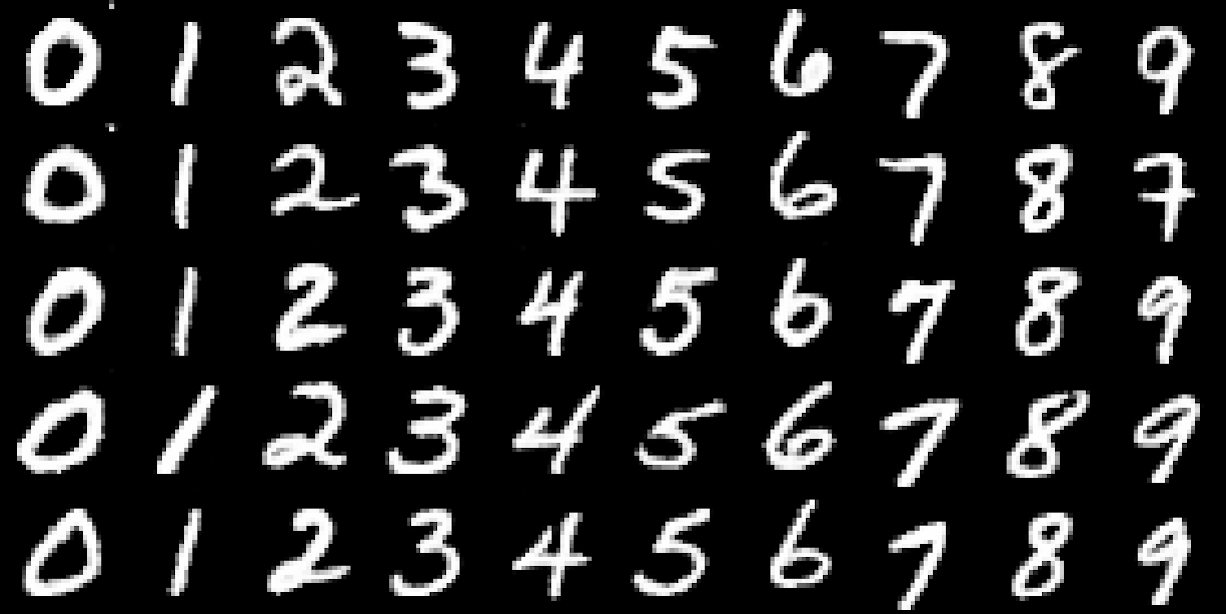
\includegraphics[width=.8\textwidth]{images/infogan_c1.png}
        \caption{Varying $\bm{c}_1 \in [0, 10]$}
    \end{subfigure}%
    \begin{subfigure}{.33\textwidth}
        \centering
        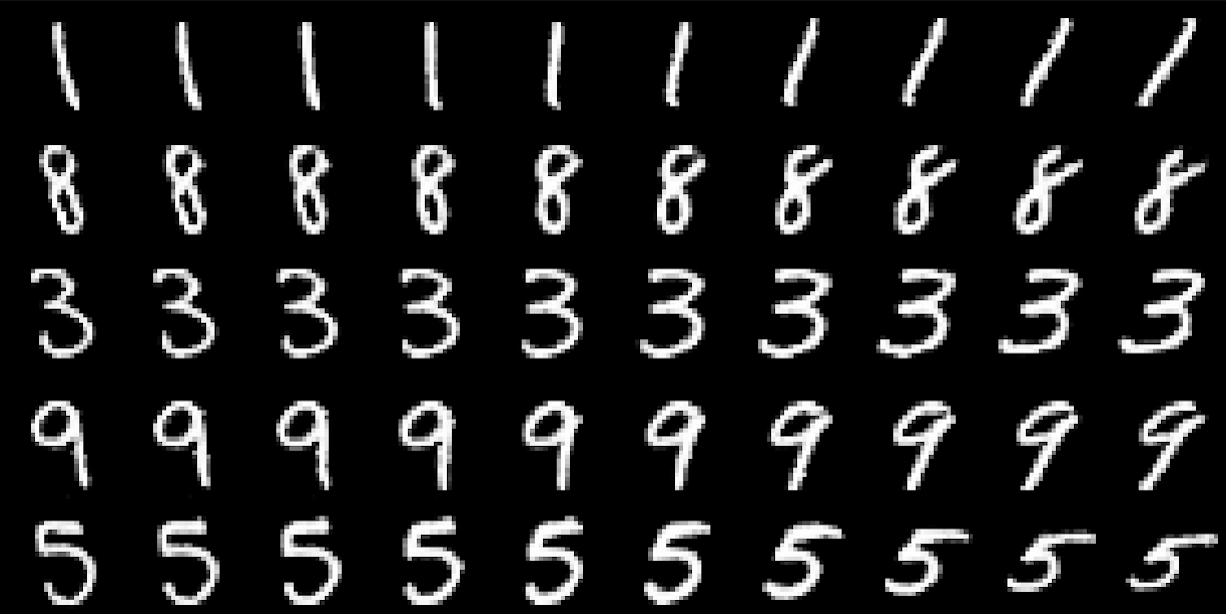
\includegraphics[width=.8\textwidth]{images/infogan_c2.png}
        \caption{Varying $\bm{c}_2 \in [-2, 2]$}
    \end{subfigure}
    \begin{subfigure}{.33\textwidth}
        \centering
        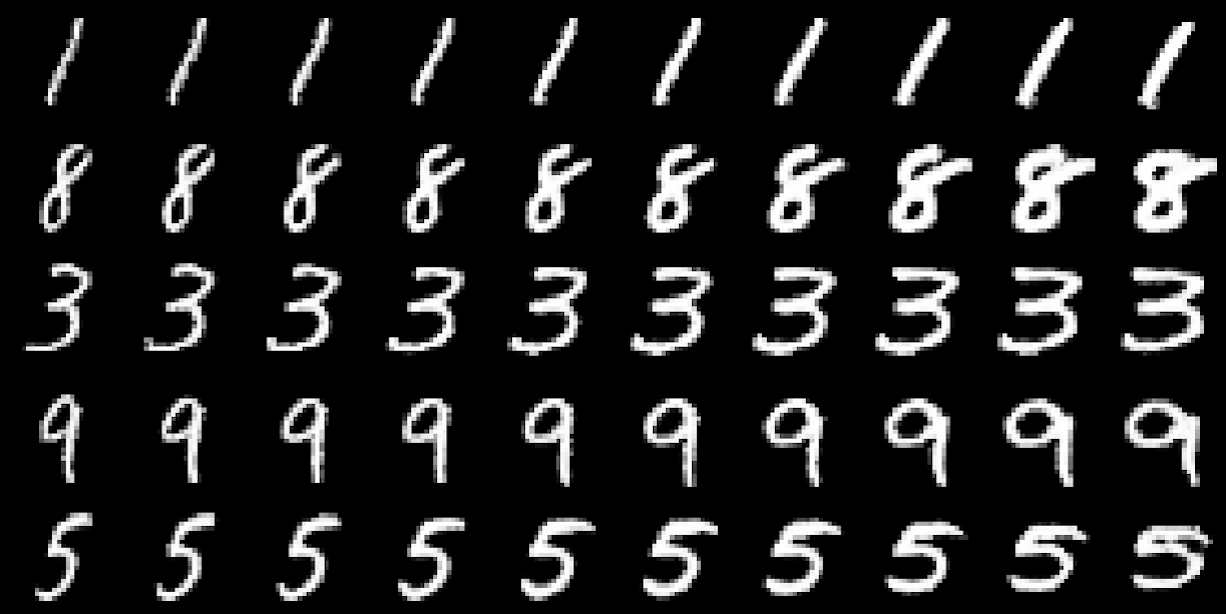
\includegraphics[width=.8\textwidth]{images/infogan_c3.png}
        \caption{Varying $\bm{c}_3 \in [-2, 2]$}
    \end{subfigure}
    \caption[InfoGAN latent space traversal]{Exploration of $\bm{c}$ for InfoGAN on MNIST by traversing either, $\bm{c}_1$, $\bm{c}_2$, or $\bm{c}_3$. Rows correspond to different noise values $\bm{z}$ but are equal for the three figures, columns correspond to different values for $\bm{c}_i$. $\bm{c}_1$ takes discrete values, $\bm{c}_2$ and $\bm{c}_3$ take continuous values. Taken from \citet{chen2016infogan}.}
    \label{fig:infogan}
\end{figure}

\say{To disentagle digit shape styles on MNIST}, \citet{chen2016infogan} choose $\bm{c}$ as three-element set $\bm{c} = (\bm{c}_1, \bm{c}_2, \bm{c}_3)$ with $\bm{c}_1$ drawn from a categorical distribution with ten categories (equal to the number of classes in MNIST) and event probability $p_i=0.1 \, \forall i \in [0, 10]$.
$\bm{c}_2$ and $\bm{c}_3$ are drawn from a uniform distribution over $[-1, 1]$.

Figure~\ref{fig:infogan} shows the latent space separability by varying the $\bm{c}_i$-values.
Noteworthy, InfoGAN seems to generalize as $\bm{c}_2$ and $\bm{c}_3$ varied between $[-2, 2]$ whereas these values took values in $[-1, 1]$ at training time.

\paragraph{StyleGAN}
StyleGAN~\citep{karras2019style} is a type of \ac{GAN} explicitly addressing \textit{latent space separability} (see Section~\ref{subsec:feature-separability}).
The term \textit{style} refers to latent space separability, i.e.~the model is capable of learning a disentanglement of images into different styles.
The styles of an image are learned at different levels.
Importantly, styles are learned in a self-supervised manner.
Therefore it is not possible to explicitly force the model to learn certain aspects of an image.
However, due to the training procedure, different styles are learned at different levels and a posterior analysis allows to identify which aspects were mainly learned on which level.
Coarse styles correspond to gender, age, or glasses.
Middle styles correspond to skin color, face form, or mouth open/closed.
Fine styles correspond mainly to hair color and lightning.

The model introduces uses some new ideas that are explained in the following.

\acp{GAN} generate new images by using some random noise $\bm{z}\in \mathcal{Z}$ as input (see Section~\ref{subsubsec:gans}).
StyleGAN uses a mapping network $f: \mathcal{Z}\mapsto \mathcal{W}$ to map the random noise to a vector $\bm{w}\in \mathcal{W}$.
With an affine transformation, the vector $w$ is then mapped to a vector $\bm{y}_i = (\bm{y}_{s,i}, \bm{y}_{b,i})$.
Different vectors $\bm{y}_i$ are fed into different layers $i$ in the generator network and control the style on this layer.

The generator network $g$ has a constant input $\bm{x}_0$ that is lower-dimensional than the final output image.
In~\citet{karras2019style}, $\bm{x}_0$ is of size $4\times 4\times 512$.
On each layer, a noise vector $\bm{\epsilon}_i$ is added, followed by an \textit{\acf{AdaIN}} operation.
The \ac{AdaIN} operation is defined as
\begin{align}
    \text{\ac{AdaIN}}(\bm{x}_i, \bm{y}) = \bm{y}_{s, i} \frac{\bm{x}_{i}-\mu\left(\bm{x}_{i}\right)}{\sigma\left(\bm{x}_{i}\right)}+\bm{y}_{b, i},
\end{align}
\citep{karras2019style} where $\mu(\cdot)$ gives the mean and $\sigma(\cdot)$ the (empirical) standard deviation.
Importantly, this operation is applied separately for each feature map of $\bm{x}_i$.

On each resolution, $g$ first applies noise addition, \ac{AdaIN}, $3\times 3$ convolution, noise addition, and one last \ac{AdaIN} operation.
Then, the image is upsampled to double size.
This process is repeated until the image has the desired output size.
\citet{karras2019style} use nine of these blocks, resulting in an output size of $1024\times 1024$.

Latent space separability is achieved by a technique called \textit{mixing regularization}.
Here, for a subset of the training images, two input vectors $\bm{z}_1$ and $\bm{z}_2$ are drawn.
During the training, a point (or layer) of $g$ is chosen by random up to which layer $\bm{z}_1$ controls the style.
After this point, the style information from $\bm{z}_2$ is fed to the network.
Randomly choosing this point \say{prevents the network from assuming that adjacent styles are correlated}~\citep{karras2019style}.

The training procedure allows using two sources for the generation.
During inference time, the crossover point can be chosen arbitrarily, i.e.~it can be controlled what styles are taken from the first and what styles are taken from the second source.

Now, $\bm{y}_i$ that are fed into the network at a low resolution (i.e. $i$ is small) control the coarse styles referred to in the beginning of the section, whereas $\bm{y}_i$ at higher layers control finer styles.

Finally, \citet{karras2019style} analyze how disentangled generations from $\mathcal{W}$-space are compared to $\mathcal{Z}$-space by means of \textit{perceptual path length}.
The perceptual path length is a measure of how much reconstructions change for small variation in the latent space.
It is calculated by moving by a small value $\epsilon$ on a path, obtained by interpolating between two random $\bm{z}_1$, $\bm{z}_2$ (or $\bm{w}_1$, $\bm{w}_2$)\footnote{Interpolation is spherical for $\bm{z}$ and interpolation for $\bm{w}$.} and taking the perceptual loss~\citep{johnson2016perceptual} between the image before moving by $\epsilon$ and after.
Finally, the mean of this value is obtained by applying the procedure for sufficiently many samples.

Using the previously described procedure, \citet{karras2019style} show that the perceptual path length is lower for interpolating in $\mathcal{W}$ compared to interpolating in $\mathcal{Z}$.
Therefore, they assumed that $\mathcal{Z}$ is more entangled than $\mathcal{W}$.

\footnote{Part on linear separability still missing}

\paragraph{\acl{LVAE}}

\begin{figure}
    \centering
    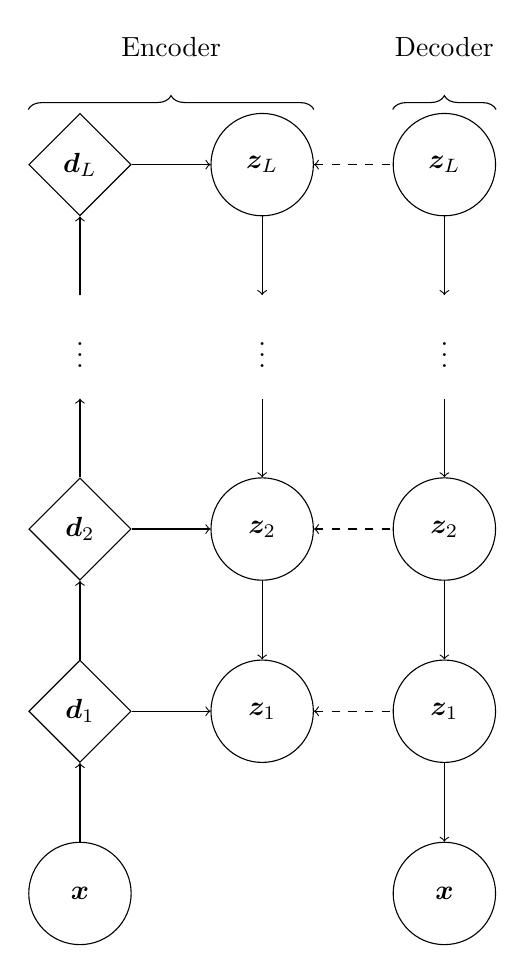
\begin{tikzpicture}
        % Nodes
        \node[draw,circle,minimum size=1.3cm] (x1) {$\bm{x}$};
        \node[draw,diamond,above=of x1,minimum size=1.3cm] (d1) {$\bm{d}_1$};
        \node[draw,diamond,above=of d1,minimum size=1.3cm] (d2) {$\bm{d}_2$};
        \node[above=of d2,minimum size=1.3cm] (ddots) {\vdots};
        \node[draw,diamond,above=of ddots,minimum size=1.3cm] (dL) {$\bm{d}_L$};
        \node[draw,circle,right=of dL,minimum size=1.3cm] (zL1) {$\bm{z}_L$};
        \node[below=of zL1,minimum size=1.3cm] (zdots1) {\vdots};
        \node[draw,circle,right=of d2,minimum size=1.3cm] (z21) {$\bm{z}_2$};
        \node[draw,circle,right=of d1,minimum size=1.3cm] (z11) {$\bm{z}_1$};

        \node[draw,circle,right=of zL1,minimum size=1.3cm] (zL2) {$\bm{z}_L$};
        \node[below=of zL2,minimum size=1.3cm] (zdots2) {\vdots};
        \node[draw,circle,right=of z21,minimum size=1.3cm] (z22) {$\bm{z}_2$};
        \node[draw,circle,right=of z11,minimum size=1.3cm] (z12) {$\bm{z}_1$};
        \node[draw,circle,below=of z12,minimum size=1.3cm] (x2) {$\bm{x}$};

        % Arrows
        \draw[->] (x1.north) -- (d1.south);
        \draw[->] (d1.north) -- (d2.south);
        \draw[->] (d2.north) -- (ddots.south);
        \draw[->] (ddots.north) -- (dL.south);

        \draw[->] (d1.east) -- (z11.west);
        \draw[->] (d2.east) -- (z21.west);
        \draw[->] (dL.east) -- (zL1.west);

        \draw[->] (zL1.south) -- (zdots1.north);
        \draw[->] (zdots1.south) -- (z21.north);
        \draw[->] (z21.south) -- (z11.north);
        \draw[->] (z22.south) -- (z12.north);
        \draw[->] (z12.south) -- (x2.north);
        \draw[->] (zL2.south) -- (zdots2.north);
        \draw[->] (zdots2.south) -- (z22.north);

        \draw[<-,dashed] (z21.east) -- (z22.west);
        \draw[<-,dashed] (z11.east) -- (z12.west);
        \draw[<-,dashed] (zL1.east) -- (zL2.west);

        \draw [decorate,decoration={brace,amplitude=5pt,raise=0.7cm},rotate=90] (dL.west) -- (zL1.east) node [black,midway,yshift=1.5cm] {Encoder};
        \draw [decorate,decoration={brace,amplitude=5pt,raise=0.7cm},rotate=90] (zL2.west) -- (zL2.east) node [black,midway,yshift=1.5cm] {Decoder};
    \end{tikzpicture}
    \caption[\ac{VLAE} structure]{\ac{LVAE} structure, adapted from \citet{sonderby2016ladder}. Solid arrows indicate feedforward connections, dashed arrows indicate weight sharing. Diamonds indicate stochastic variables, circles deterministic variables.}
    \label{fig:lvae}
\end{figure}

\aclp{LVAE}~\citep{sonderby2016ladder} address the problem of hierarchical learning in \acp{VAE}.
Hierarchical \acp{VAE} only use the first few layers to learn meaningful semantics of an input.
In case of \citet{sonderby2016ladder}, the first two layers are sufficient.
\citet{zhao2017learning} state that, given a sufficiently large encoder network in the first layer, the first layer learns all the semantics.
While this is not always true, they \say{demonstrate that this phenomen occurs in practice [\ldots]}.

\acp{LVAE} is a model designed to, instead of using just the first few layers, use all embedding layers to learn a representation.
They do this by passing information top-down in the inference network.
\begin{figure}
    \centering
    
\includegraphics[width=0.2\textwidth]{images/gerben.png}
    \caption[Context-Dependent Semantic Ambiguity]{Illustration of context-dependent semantic ambiguity. Taken from \citet[p. 61]{van2016auto}}
    \label{fig:gerben_ambiguity}
\end{figure}
Figure~\ref{fig:gerben_ambiguity} gives an intuition why passing information top-down can be advantegous.
Here, the two rows show two different alphanumeric strings.
Apparently, the first row shows a sequence of alphabetic characters (\say{GERBEN}) whereas the second row shows a sequence of numeric characters (\say{10 11 12 13 14 15}).
However, the \say{R} and the \say{B} in the first row are the exact same symbols as the \say{12} and the \say{13} in the second one.
A pure feed-forward systems would be unable to discriminate between the low-level features \textit{R} and \textit{13}.
Incorporating high-level features like \textit{alphabetic string} helps to improve the posterior low-level feature representation.
Furthermore, the additional top-down pass is more biologically plausible compared to a pure feedforward network~\citep{rodriguez2015hierarchical}.
\citet{rodriguez2015hierarchical} explicitly discuss \say{the need for top-down priming or attention}.

Unlike hierarchical \acp{VAE}, \acp{LVAE} do not use the output of lower stochastic embedding layers as input for higher layers.
Instead, they use a deterministic multi-layer network in the encoder (see Figure~\ref{fig:lvae}) and pass information from intermediate layers to the stochastic embedding layers.
\begin{align}
    \bm{d}_i &= \text{NN}(\bm{d}_{i-1})\\
    \hat{\bm{\mu}}_{q,i}&=\text{NN}(\bm{d}_i)\\
    \hat{\bm{\sigma}}^2_{q,i}&=\text{NN}(\bm{d}_i)
\end{align}
Output from higher stochastic embedding layers is passed to lower layers via the decoder $p$:
\begin{align}
    \bm{\sigma}_{q,i}&=\frac{1}{\hat{\bm{\sigma}}^{-2}_{q,i}+\hat{\bm{\sigma}}^{-2}_{p,i}}\\
    \bm{\mu}_{q,i}&=\frac{\hat{\bm{\mu}}_{q,i}\hat{\bm{\sigma}}^{-2}_{q,i}+\hat{\bm{\mu}}_{p,i}\hat{\bm{\sigma}}^{-2}_{p,i}}{\hat{\bm{\sigma}}^{-2}_{q,i}+\hat{\bm{\sigma}}^{-2}_{p,i}}
\end{align}
The latent variables then are sampled conditionally:
\begin{align}
    q(\bm{z}_i|\cdot)=\mathcal{N}(\bm{z}_i|\bm{\mu}_{q,i},\bm{\sigma}^2_{q,i})
\end{align}

\citet{sonderby2016ladder} show that gradually increasing the weight of the KL-term in the \ac{VAE} training criterion leads to a better usage of the latent spaces in terms of active units.
Without this \textit{warm-up} phase, \acp{VAE} show many inactive units.
\citet{sonderby2016ladder} discuss that \acp{VAE} show this behavior because it allows them to minimize the KL-term in the \ac{VAE} loss function fast.

Using batch-normalization and warm-up alone already leads to more meaningful representations in the higher layers of a hierarchical VAE~\citep{sonderby2016ladder}.
Using all these techniques on the \ac{LVAE} model allows meaningful representations in even higher layers compared to a hierarchical VAE\footnote{In \citet{sonderby2016ladder}, a hierarchical \ac{VAE} with batch-normalization and warm-up learns meaningful representations up to the fourth layer where as 5-layer \ac{LVAE} also learns meaningful representations in the fifth layers. Deeper models were not investigated.}.

\paragraph{\acl{VLAE}}

\begin{figure}
    \centering
    \begin{subfigure}{.45\textwidth}
        \centering
        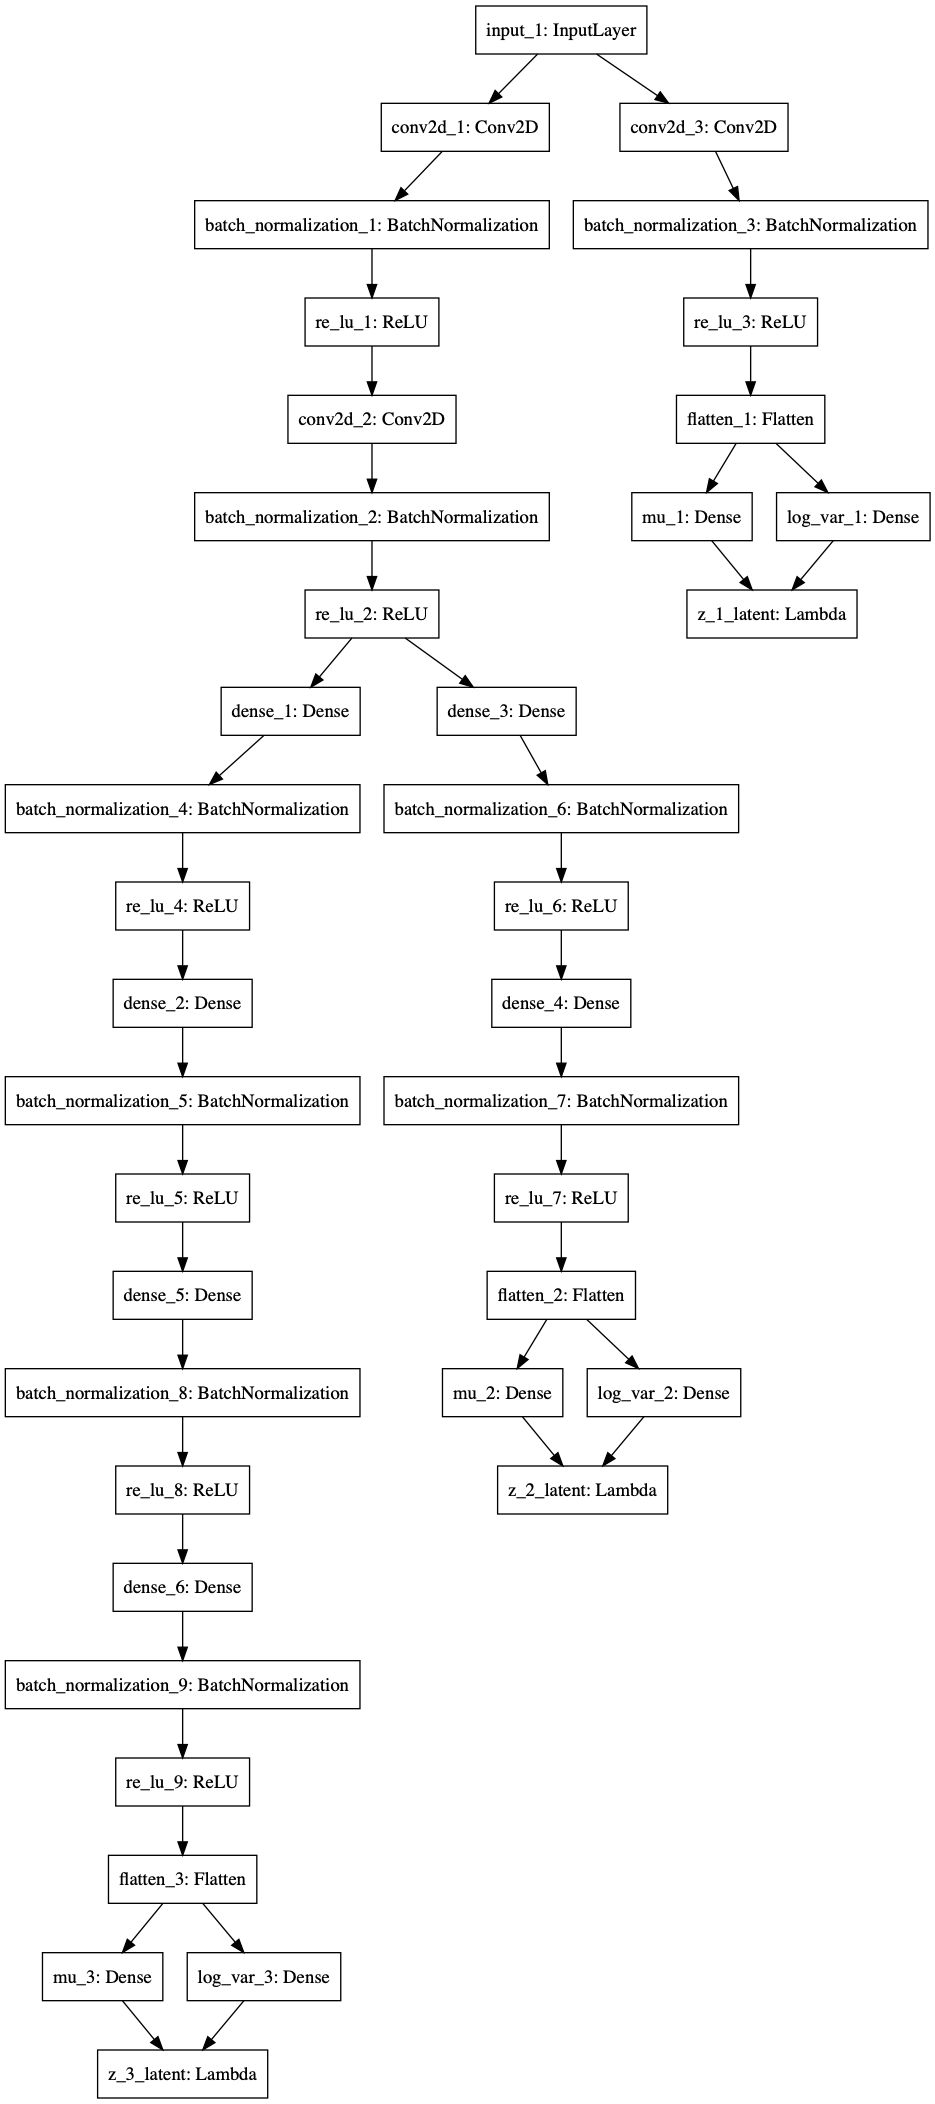
\includegraphics[height=.8\textheight]{images/vlae_encoder.png}
        \caption{Varying $\bm{c}_1 \in [0, 10]$}
    \end{subfigure}%
    \begin{subfigure}{.45\textwidth}
        \centering
        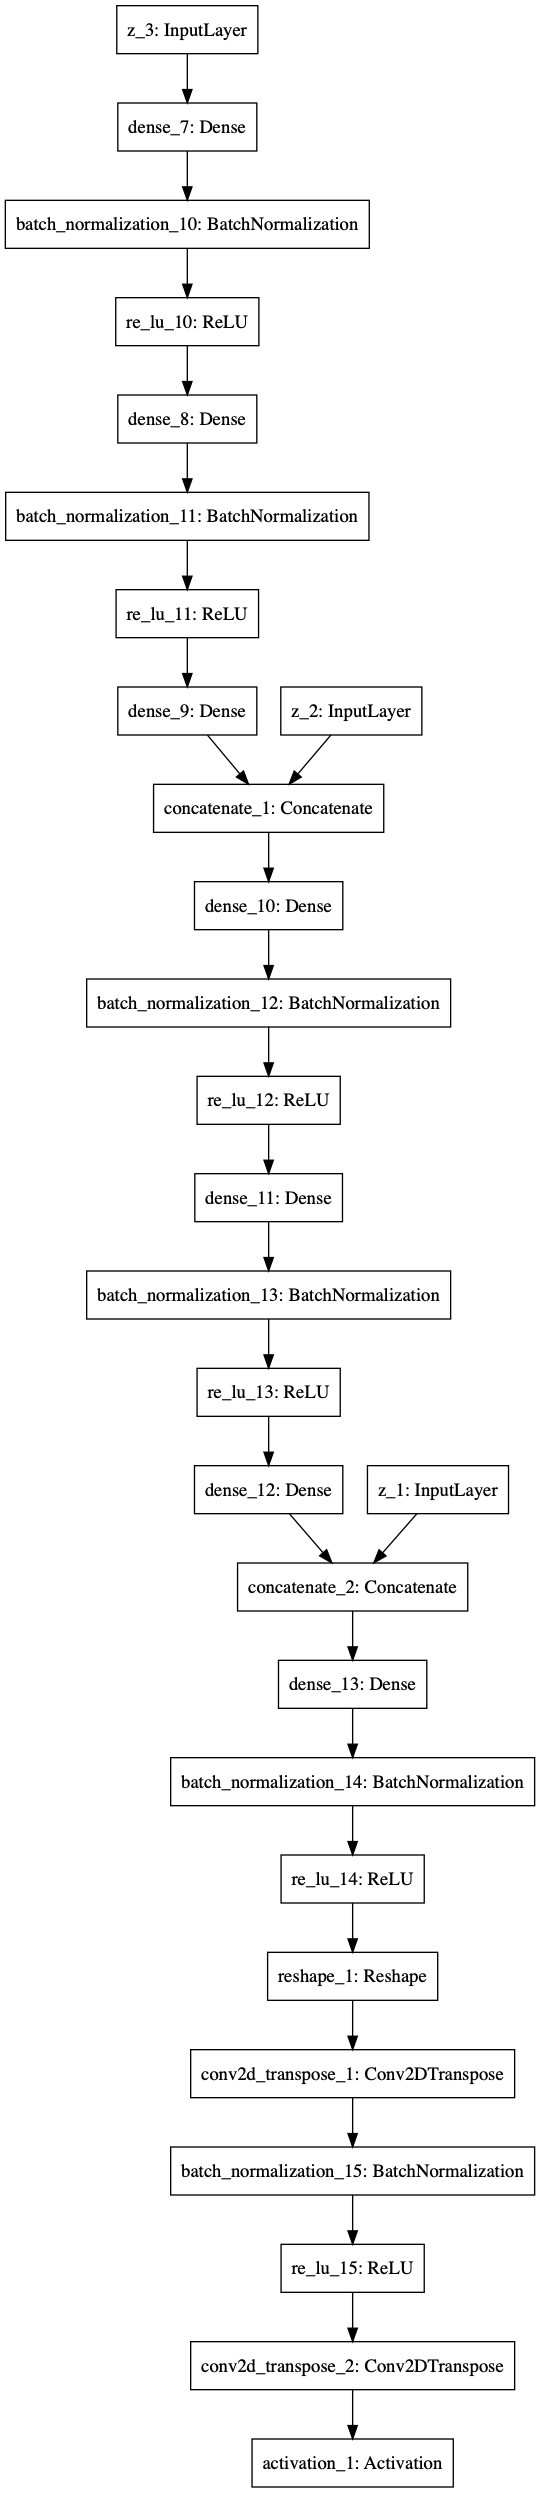
\includegraphics[height=.8\textheight]{images/vlae_decoder.png}
        \caption{Varying $\bm{c}_2 \in [-2, 2]$}
    \end{subfigure}
    \caption[\ac{VLAE} structure]{Structure of the \ac{VLAE} model}
    \label{fig:vlae_structure}
\end{figure}

Unlike the \ac{LVAE}, the \ac{VLAE}~\citep{zhao2017learning} is a pure feedforward network.
It's design is driven by the idea that \say{[i]f $\bm{z}_i$ is more abstract than $\bm{z}_j$, then the inference mapping $q(\bm{z}_i|\bm{x})$ and generative mapping when other layers are fixed $p(\bm{x}|\bm{z}_i, \bm{z}_{\neg i}=z^0_{\neg i})$ requires a more expressive network to capture}~\citep{zhao2017learning}.
Figure~\ref{fig:vlae_structure} shows an exemplary network structure of a \ac{VLAE}.
Early embedding layers like $\bm{z}_1$ are equipped with a less expressive network that, according to \citet{zhao2017learning}, should not allow to learn abstract features\footnote{In case of \textsc{Mnist}, more abstract features are for example the digit identity.}.

These assumptions are discussed in Section~\ref{subseq:criticism_vlae}.

\paragraph{$\beta$-VAE}

Consider Equation~\ref{eq:elbo_error_term} describing the loss function in a \ac{VAE}.
\citet{higgins2017beta} discovered that weighting both terms, the KL-divergence and the reconstruction loss, equally leads to suboptimal results in terms of \textit{feature disentanglement}.
They therefore formulated the $\beta$-VAE learning objective that adds an additional hyperparameter $\beta$ to the loss function, controlling the relative weights of the two terms:
\begin{align}
    \mathbb{E}_{q_{\phi}(\bm{z} | \bm{x})}\left[\log p_{\theta}(\bm{x} | \bm{z})\right]-\beta \kldiv{q_{\phi}(\bm{z} | \bm{x})}{p(\bm{z})}
\end{align}

A value $\beta > 1$ puts more emphasis on the KL-term compared to the original \ac{VAE} loss function ($\beta = 1$).
\citet{higgins2017beta} state that this could lead to better feature disentanglement because the KL-term \say{encourages conditional independence in $q_\phi(\bm{z}|\bm{x})$}~\citep{higgins2017beta}.
This requires that some factors of the data are conditionally independent, \citet{higgins2017beta}, however, show empirically that this often is the case.

Setting $\beta > 1$ also lowers the influence of the reconstruction error in the \ac{VAE} training objective.
This leads to worse reconstructions.
The right parameter choice, therefore, is context dependent.

\paragraph{\ac{VAE}-\ac{GAN}}
\ac{VAE}-\acp{GAN}~\citep{larsen2015autoencoding} are a variation of \acp{VAE} specifically designed to replace the pixel-wise reconstruction loss.
Even on highly curated datasets such as \textsc{Mnist} (\textbf{REF}), \acp{VAE} tend to generate blurry images.
The design of \ac{VAE}-\acp{GAN} is based on the assumption that the pixel-wise loss in the \ac{VAE} training objective (see Equation~\ref{eq:log_normal_distr}) is the reason for blurry output images.
\citet{larsen2015autoencoding}~motivate this by stating that even small translations result in a high pixel-wise loss\footnote{This depends on the image's frequency as well as the variance of the pixel intensities.}.

Instead of measuring the \ac{MSE} between the true and the generated image, \ac{VAE}-\acp{GAN} train a discriminator network to distinguish between generated and true images, i.e.~to maximize
\begin{align}
    \mathcal{L}_{\mathrm{GAN}}=\log (D(\bm{x}))+\log (1-D(G(\bm{z}))) \label{eq:vae_gan_l_gan}
\end{align}
where $D$ and $G$ are the discriminator/generator networks, $\bm{x}$ an input image and $\bm{z}\sim \mathcal{N}(\bm{0},\bm{I})$ a random Gaussian sample.
For \ac{VAE}-\acp{GAN}, the generator network is nothing but the decoder network whereas the discriminator network is an additional network that does not exist for \acp{VAE}.

Equation~\ref{eq:vae_gan_l_gan} is sufficient to train the discriminator network.
However, it does not force $p(\bm{x}) \approx \mathcal{N}(\bm{0},\bm{I})$ nor does it force reconstructions to resemble the input image.

The latter is achieved by introducing an additional loss term
\begin{align}
    \mathcal{L}_{\text {llike}}^{\text {D}}=-\mathbb{E}_{q(\bm{z} | \bm{x})}\left[\log p\left(\operatorname{D}_{l}(\bm{x}) | \bm{z}\right)\right]
\end{align}
penalizing differences of intermediate discriminator layer activations between $\bm{x}$ and the reconstruction $\tilde{\bm{x}}$ of $\bm{x}$.
The former, forcing $p(\bm{x}) \approx \mathcal{N}(\bm{0},\bm{I})$, is achieved by minimizing the \ac{KL}-divergence as in Equation~\ref{eq:elbo_error_term}:
\begin{align}
    \mathcal{L}_{\text {prior }}=\kldiv{q(\boldsymbol{z} | \boldsymbol{x})}{p(\boldsymbol{z})}
\end{align}

The encoder is trained to minimize $\mathcal{L}_{\text {prior }} +  \mathcal{L}_{\text {llike}}^{\text {D}}$, the decoder to minimize $\gamma \mathcal{L}_{\text {llike}}^{\text {D}} - \mathcal{L}_\mathrm{GAN}$, and the discriminator to minimize $-\mathcal{L}_\mathrm{GAN}$.
Setting $\gamma = 0.75$ led to training convergence for the experiments performed for this thesis.

\citet{larsen2015autoencoding}~show that this training procedure leads to less blurry reconstructions.

\paragraph{Adversarial Latent Autoencoder}
\begin{figure}
    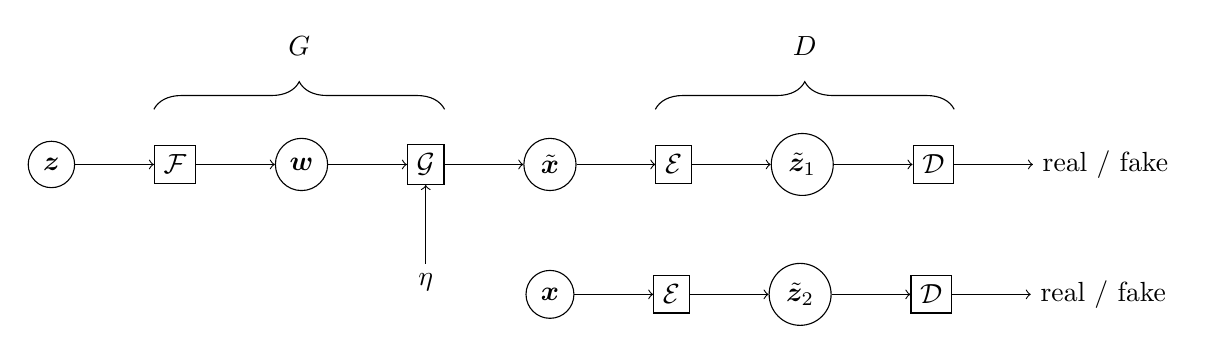
\begin{tikzpicture}
        % Nodes
        \node[draw,circle] (z) {$\bm{z}$};
        \node[draw,rectangle,right=of z] (F) {$\mathcal{F}$};
        \node[draw,circle,right=of F] (w) {$\bm{w}$};
        \node[draw,rectangle,right=of w] (G) {$\mathcal{G}$};
        \node[draw,circle,right=of G] (xt) {$\tilde{\bm{x}}$};
        \node[draw,rectangle,right=of xt] (E1) {$\mathcal{E}$};
        \node[draw,circle,right=of E1] (zt1) {$\tilde{\bm{z}}_1$};
        \node[draw,rectangle,right=of zt1] (D1) {$\mathcal{D}$};
        \node[right= of D1] (realfake1) {real / fake};
        \node[below=of G] (eta) {$\eta$};

        \node[draw,circle,below=of xt] (x) {$\bm{x}$};
        \node[draw,rectangle,right=of x] (E2) {$\mathcal{E}$};
        \node[draw,circle,right=of E2] (zt2) {$\tilde{\bm{z}}_2$};
        \node[draw,rectangle,right=of zt2] (D2) {$\mathcal{D}$};
        \node[right= of D2] (realfake2) {real / fake};
        % Arrows
        \draw[->] (z.east) -- (F.west);
        \draw[->] (F.east) -- (w.west);
        \draw[->] (w.east) -- (G.west);
        \draw[->] (G.east) -- (xt.west);
        \draw[->] (xt.east) -- (E1.west);
        \draw[->] (E1.east) -- (zt1.west);
        \draw[->] (zt1.east) -- (D1.west);
        \draw[->] (D1.east) -- (realfake1.west);
        \draw[->] (eta.north) -- (G.south);

        \draw[->] (x.east) -- (E2.west);
        \draw[->] (E2.east) -- (zt2.west);
        \draw[->] (zt2.east) -- (D2.west);
        \draw[->] (D2.east) -- (realfake2.west);

        \draw [decorate,decoration={brace,amplitude=10pt,raise=0.7cm},rotate=90] (F.west) -- (G.east) node [black,midway,yshift=1.5cm] {$G$};
        \draw [decorate,decoration={brace,amplitude=10pt,raise=0.7cm},rotate=90] (E1.west) -- (D1.east) node [black,midway,yshift=1.5cm] {$D$};
    \end{tikzpicture}
    \caption[\ac{ALAE} training]{Training of \ac{ALAE}, adapted from \citet{pidhorskyi2020adversarial}}
    \label{fig:alae_flow}
\end{figure}
Similar to \ac{VAE}-\acp{GAN}, \acfp{ALAE}~\citep{pidhorskyi2020adversarial} are a hybrid model between \acp{VAE} and \acp{GAN}.
\acp{ALAE} are not based on variational inference but on \acp{GAN}.

The starting point of the \ac{ALAE} model is to decompose both, the generator $G$ and discriminator $D$, into two parts, i.e.~$G=\mathcal{G}\circ \mathcal{F}$ and $D=\mathcal{D}\circ \mathcal{E}$ (see Figure~\ref{fig:alae_flow}).
$\mathcal{G}$ uses noise $\eta$ as an additional input.
$\mathcal{F}$ maps the Gaussian random noise $\bm{z} \sim \mathcal{N}(\bm{0}, \bm{I})$ to another latent representation $\bm{w}$.
The loss function requires the outputs of $\mathcal{F}$ and $\mathcal{E}$ to be similar in terms of the $l^2$-norm.
Apart from this, the $\bm{w}$-space is unregularized.
In addition to the $l^2$-loss, the model is optimized towards minimizing the discriminator and the generator loss.

Because $p_{\mathcal{E}}(w) \approx p_{\mathcal{F}}(w)$, \ac{ALAE} can generate reconstructions by
\begin{align}
    \bm{x}\approx (\mathcal{E}\circ \mathcal{G}_\eta)(\bm{x})
\end{align}
$\mathcal{G}_\eta$ here indicates that $\mathcal{G}$ uses $\eta$ as an additional input.

Furthermore, just like for the \ac{VAE}, the Gaussian latent space $Z$ can be traversed to generate new samples by
\begin{align}
    \bm{x}_{\text{new}} = (\mathcal{F}\circ \mathcal{G}_\eta)(\bm{z})
\end{align}

\citet{pidhorskyi2020adversarial} show that (linearly) interpolating in $\bm{w}$-space yields smoother transitions than interpolation between two corresponding points in $\bm{z}$-space.
This indicates that the $\bm{w}$-space is less entangled than the $\bm{z}$-space~\citep{shao2018riemannian,arvanitidis2017latent}.
However, traversing the $\bm{w}$-space is not easily possible as its structure is unknown.
Compared to \acp{VAE} where a linear interpolation between points in the latent $\bm{z}$-space leads to an almost geodesic path in $\bm{x}$-space\footnote{Therefore, points that are close in $\bm{z}$-space of an \ac{VAE} lead to images that are close in the feature space.}, the mapping function $\mathcal{F}$ seems to be non-smooth.
Therefore, traversing $\bm{z}$ for an \ac{ALAE} seems to lead to a non-smooth path in the feature space.

Compared to the \ac{VAE} that uses a pixelwise loss on the reconstructions, \ac{ALAE} penalizes the $l^2$-norm of $\bm{w}$ and $\tilde{\bm{w}}$.
Except for this loss, \ac{ALAE} by no means forces the input to be similar to the reconstruction.
This mitigates the problem of the pixelwise loss in \acp{VAE} that is assumed to be the reason for blurry reconstructions.

\paragraph{Other stuff}
\textbf{DRAFT!}
\begin{itemize}
    \item \citet{tschannen2018recent} give an overview over \say{recent advances in autoencoder-based representation learning}
    \item Discuss VAEs on sequences of images.
    \item Check \citet{pidhorskyi2020adversarial} for more related work.
\end{itemize}

\subsection{Latent Space Disentanglement}\label{subsec:feature-disentanglement}
\textit{Latent Space Disentanglement} is a concept not to be confused with \textit{Latent Space Separability} (see Section~\ref{subsec:feature-separability}).
These two concepts are explained in the following.

\begin{figure}
    \centering
    \begin{subfigure}{.3\textwidth}
        \centering
        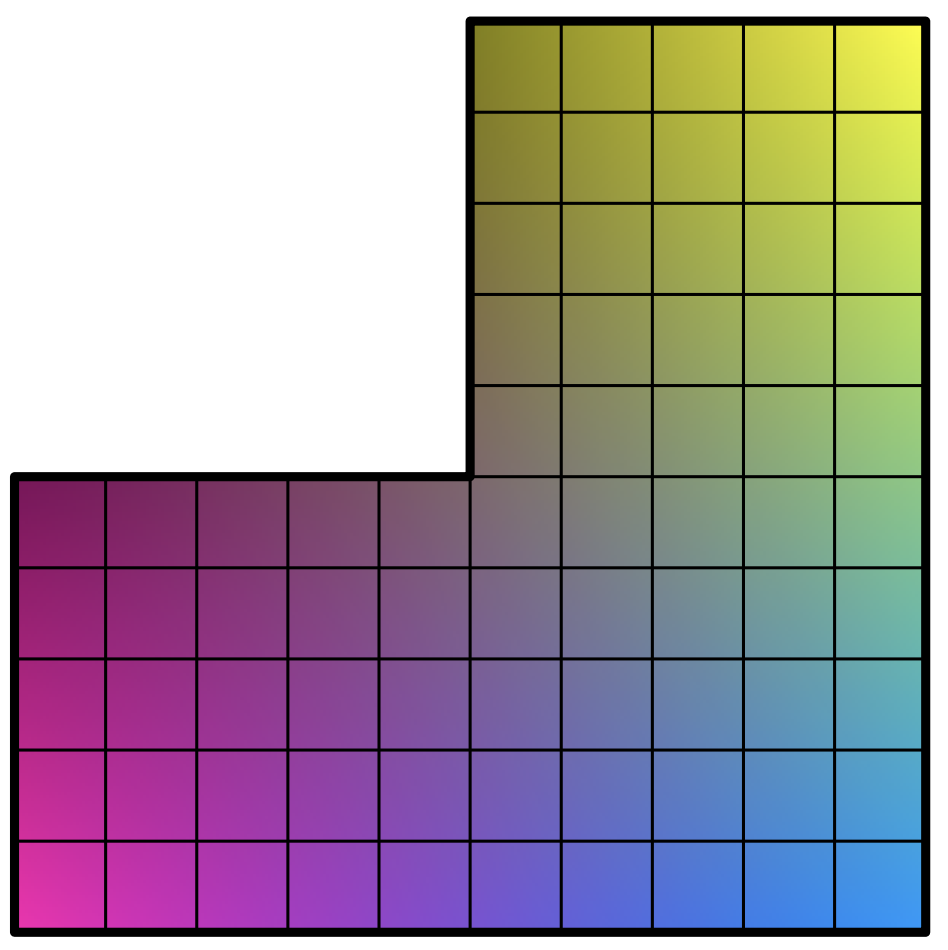
\includegraphics[width=\textwidth]{images/latent_space_disentanglement_a.png}
        \caption{\say{Distribution of features in the training set}~\citep{karras2019style}}
        \label{fig:feature_space_disentanglement_a}
    \end{subfigure}%
    \hfill
    \begin{subfigure}{.3\textwidth}
        \centering
        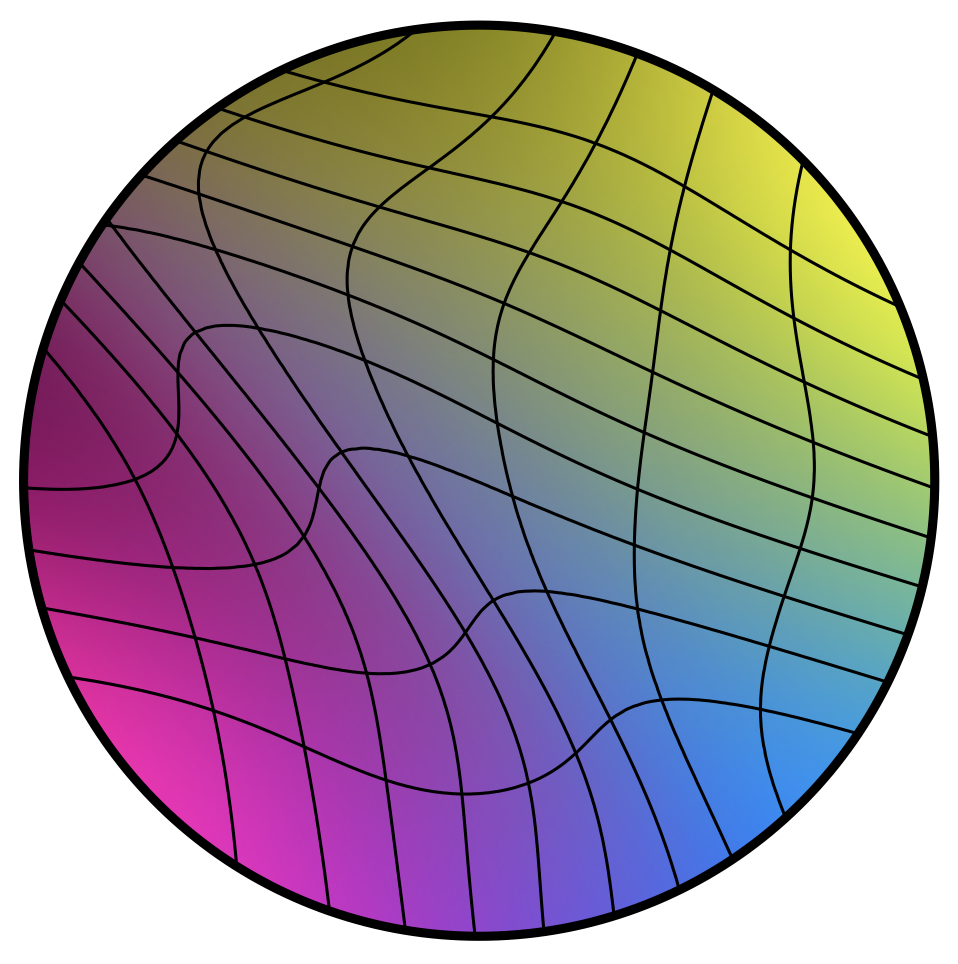
\includegraphics[width=\textwidth]{images/latent_space_disentanglement_b.png}
        \caption{Mapping from latent space to feature space}
        \label{fig:feature_space_disentanglement_b}
    \end{subfigure}
    \caption{The problem of latent space entanglement (taken from \citet{karras2019style})}
    \label{fig:feature_space_disentanglement}
\end{figure}

Consider Figure~\ref{fig:feature_space_disentanglement_a} and assume a dataset of males containing only two factors of variation, e.g. age ($x$-axis from older to younger) and voice level ($y$-axis, bottom-up from lower to higher).
The missing square in the upper left is the combination \say{old and high voice level} that is missing in the dataset.
Now, consider Figure~\ref{fig:feature_space_disentanglement_b} showing a mapping from a latent space to the feature space.
The upper left square in Figure~\ref{fig:feature_space_disentanglement_a} is not present in this latent space.
This leads to \textit{Latent Space Entanglement}: when interpolating in the latent space, there are paths along which the factors of variation change faster than for other paths.

Different methods have been proposed to measure the degree of latent space entanglement.
One approach is to measure the degree by which a generated image changes as the latent space is entangled (\textit{Perceptual Path Length})~\citep{karras2019style}.
If the latent space is entangled, this value on average should be higher compared to a disentangled space.

Another approach is \textit{Linear Separability}~\citep{karras2019style}, measuring how well sets of points can be separated by a linear hyperplane.

\citet{kim2018disentangling} propose to generate data by fixing one factor of variation (for example one dimension in the latent space) and randomly sampling from others.
If the latent space is disentangled, there should be one or multiple almost invariant dimensions in the generated data that attribute to the fixed factor of variation.

\subsection{Latent Space Separability}\label{subsec:feature-separability}

\textit{Latent Space Separability} is related to Latent Space Disentanglement but it is used in a stricter sense in the course of this thesis.
Whereas Latent Space Disentanglement was mainly motivated by the disentanglement of one latent space, Latent Space Separability is concerned with splitting up the latent space representation of features into multiple levels of latent spaces.
If successful, Latent Space Separability allows to directly control the factors of variation without the need to find the subspace in one latent space controlling this factor.

For example, \textit{InfoGAN} (see Section~\ref{subsubsec:representation_learning}) is based on this principle.
Another example is \ac{VLAE}.

Importantly, Latent Space Separability is supposed to have two properties: \textit{Consistency} and \textit{Restrictiveness} as defined in \citet{Shu2020Weakly}.
Consistency means that if only one factor of variation is varied (e.g. the factor that attributes to an object's size) and the others are fixed, generated items only change with respect to this very factor but not to other factors (i.e. only the object's size is changing but not it's shape).
Restrictiveness means that if, again, only one factor $i$ of variation is varied, the choice of the other factors should not affect the models measurement of the $i$-th factor.
For example, if factor $i$ again encodes an objects size, the same value of factor $i$ should always encode the same size, irrespective of the choice if the other factors~\citep{Shu2020Weakly}.

Strictly unsupervised approaches are not guaranteed to have both of the properties.
Suprisingly, however, most unsupervised approaches for Latent Space Separability empirically show to have these properties to a high degree~\citep{Shu2020Weakly}.

\subsection{Semantic Representations}\label{subsec:semantic-representations}
For the term \textit{Semantic Representations}, a universally accepted definition yet has to be found.
\textit{Semantics} is defined\footnote{\href{https://www.lexico.com/en/definition/semantics}{https://www.lexico.com/en/definition/semantics}, last access: 21/06/2020} as
\begin{displayquote}
    The branch of linguistics and logic concerned with meaning. There are a number of branches and subbranches of semantics, including formal semantics, which studies the logical aspects of meaning, such as sense, reference, implication, and logical form, lexical semantics, which studies word meanings and word relations, and conceptual semantics, which studies the cognitive structure of meaning.
\end{displayquote}
This thesis is less concerned with linguistics but with \textit{meanings} and \textit{relations}, not of language but of \textbf{images}.
A general definition of \textit{Semantic Representations}, however, should not be restricted to words or images.
It should incorporate all kinds of concepts a human can form of a perception.

In the course of this thesis, \textit{Semantic Representations} are somewhat related to \textit{Word Embeddings} in \ac{NLP}.
Word embeddings~\citep{mikolov2013efficient} are a vectorized representation of words in a vector space.
The training procedure learns a mapping from word into the latent space such that the word's position itself has meaning.
One prominent example is that the vector space allows \say{simple algebraic operations[...]. [I]t was shown for example that \textit{vector}(\say{King}) - \textit{vector}(\say{Man}) + \textit{vector}(\say{Woman}) results in a vector that is closest to the vector representation of the word \textit{Queen} [...]}~\citep{mikolov2013efficient}.

Just like the brain maps similar visual stimuli to neurons close to one another, a semantic representation should be an encoding of the concept where encodings of similar concepts are close to one another according to some distance metric.

Unfortunately, a dense vector (as in word embeddings) as a semantic representation is rather unrelated to a subpopulation of active neurons.
The question of how to obtain good semantic representations remains.
One requirement could be that a model leading to semantic representations should behave like the biological example.

It has been reported that the activations of hidden layers in supervised \acp{CNN} explain \ac{IT} cortical representation~\citep{khaligh2014deep,cadieu2014deep}.

Additionally, there is some evidence that unsupervised models do not explain \ac{IT} cortical representation (or by far worse than supervised models)~\citep{khaligh2014deep}.
Finally, it remains unclear if Gabor wavelets emerge in unsupervised \acp{CNN}~\citep{han2019variational}.
There are, however, unsupervised models that learn Gabor wavelets~\citep{berkes2005slow}.




\section{Methods}\label{sec:methods}
The following Sections describe the methods used in the course of this thesis.

\subsection{Implementation Details}\label{subsec:implementation-details}

All models are implemented with Keras\footnote{\href{https://keras.io/}{https://keras.io/}, last access: 07/01/2020} in Version 2.2.4 using the TensorFlow\footnote{\href{https://www.tensorflow.org/}{https://www.tensorflow.org/}, last access: 07/01/2020} backend in Version 1.15..
The models are trained on Tesla V100-DGXS GPUs with 16GB of RAM.
The model code can be found under \href{https://github.com/LeoIV/master-thesis-leonard}{https://github.com/LeoIV/master-thesis-leonard}.

\subsection{Datasets}\label{subsec:datasets}

Five different datasets were used to train the models.
Four of the datasets contain images of different sizes, the fifth dataset provides additional labels for the \textsc{Mnist} dataset.
The images were resized to match the model's expected input sizes using Lanczos interpolation~\citep[pp. 223, ff]{burger2009principles}.

\subsubsection{CelebA}\label{subsubsec:celeba_dataset}

\begin{wrapfigure}[14]{R}{0.3\textwidth}
    \begin{center}
        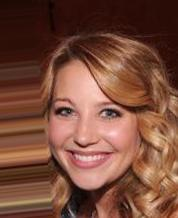
\includegraphics[width=0.28\textwidth]{images/celeba_sample_63.jpg}
    \end{center}
    \caption[CelebA dataset sample image]{A sample image from the CelebA dataset.}
    \label{fig:celeba_sample}
\end{wrapfigure}

The \textit{CelebA} dataset~\citep{liu2015faceattributes} consists of 202,599 RGB images of size 178 x 218 pixels representing celebrities, as well as 40 binary attributes.
The images belong to 10.177 unique identities\footnote{The identities are not revealed.} as well as five \say{landmark annotations}.
They are aligned and cropped resulting in images of same size always showing only one face (see Figure~\ref{fig:celeba_sample} for an example).
The landmark annotations give the positions of facial attributes in the image; the left and right eye, the nose, and the left and right corner of the mouth.
The binary attributes indicate if the image has certain characteristics, for example if the person wears eyeglasses, has black hair, is smiling\footnote{See \href{https://www.kaggle.com/jessicali9530/celeba-dataset\#list\_attr\_celeba.csv}{https://www.kaggle.com/jessicali9530/celeba-dataset\#list\_attr\_celeba.csv} for a complete list of the attributes, login required. Last access: 12/02/2020.}.

\subsubsection{ImageNet}\label{ssec:imagenet}

ImageNet\footnote{\href{http://image-net.org/}{http://image-net.org/}, last access: 12/02/2020.} is a large-scale \say{image database organized according to the WordNet hierarchy}~\citep{imagenet_cvpr09}.
It contains of over 14 million images as of February 2020.
According to WordNet\footnote{See \href{https://wordnet.princeton.edu/}{https://wordnet.princeton.edu/}, last access: 12/02/2020.}, the images are subdivided into groups called \say{synsets}~\citep{imagenet_cvpr09} on different levels of granularity.
For example, the group \textit{woman, adult female} is subordinated to \textit{person, individual, someone, somebody, mortal, soul} and is further subdivided into groups like \textit{old woman} or \textit{lady} \footnote{ImageNet 2011 Fall Release, \href{http://image-net.org/explore}{http://image-net.org/explore}, last access: 12/02/2020.}

A smaller version of ImageNet, commonly called \textit{ILSVRC2012} has been used for \ac{ILSVRC2017}~\citep{ILSVRC15}, consisting of approximately 1,3 million images from 1000 different classes, that were selected, such that \say{there is no overlap between synsets: for any synsets $i$ and $j$, $i$ is not an ancestor of $j$ in the ImageNet hierarchy}~\citep{imagenet_cvpr09}.

This curated version is commonly used as a baseline (\textbf{refs}).

\subsubsection{Mnist}\label{subsubsec:mnist}

\begin{wrapfigure}[9]{R}{0.2\textwidth}
    \begin{center}
        
\includegraphics[width=0.18\textwidth]{images/mnist_sample.png}
    \end{center}
    \caption[\textsc{Mnist} dataset sample image]{A sample image from the \textsc{Mnist} dataset.}
    \label{fig:mnist_sample}
\end{wrapfigure}

\textsc{Mnist}\footnote{\href{http://yann.lecun.com/exdb/mnist/}{http://yann.lecun.com/exdb/mnist/}, last access: 23/04/2020}~\citep{lecun1998gradient} is a widely-used dataset of hand-written digits.
The data is subdivided into a training set of 60.000 images and a test set containing 10.000 images.
The digits are all of the same size and centered.
The samples are grayscale images of size $28\times 28$pixels.

\subsubsection{Morpho-\textsc{Mnist}}\label{subsubsec:morphomnist}

\begin{figure}
    \centering
    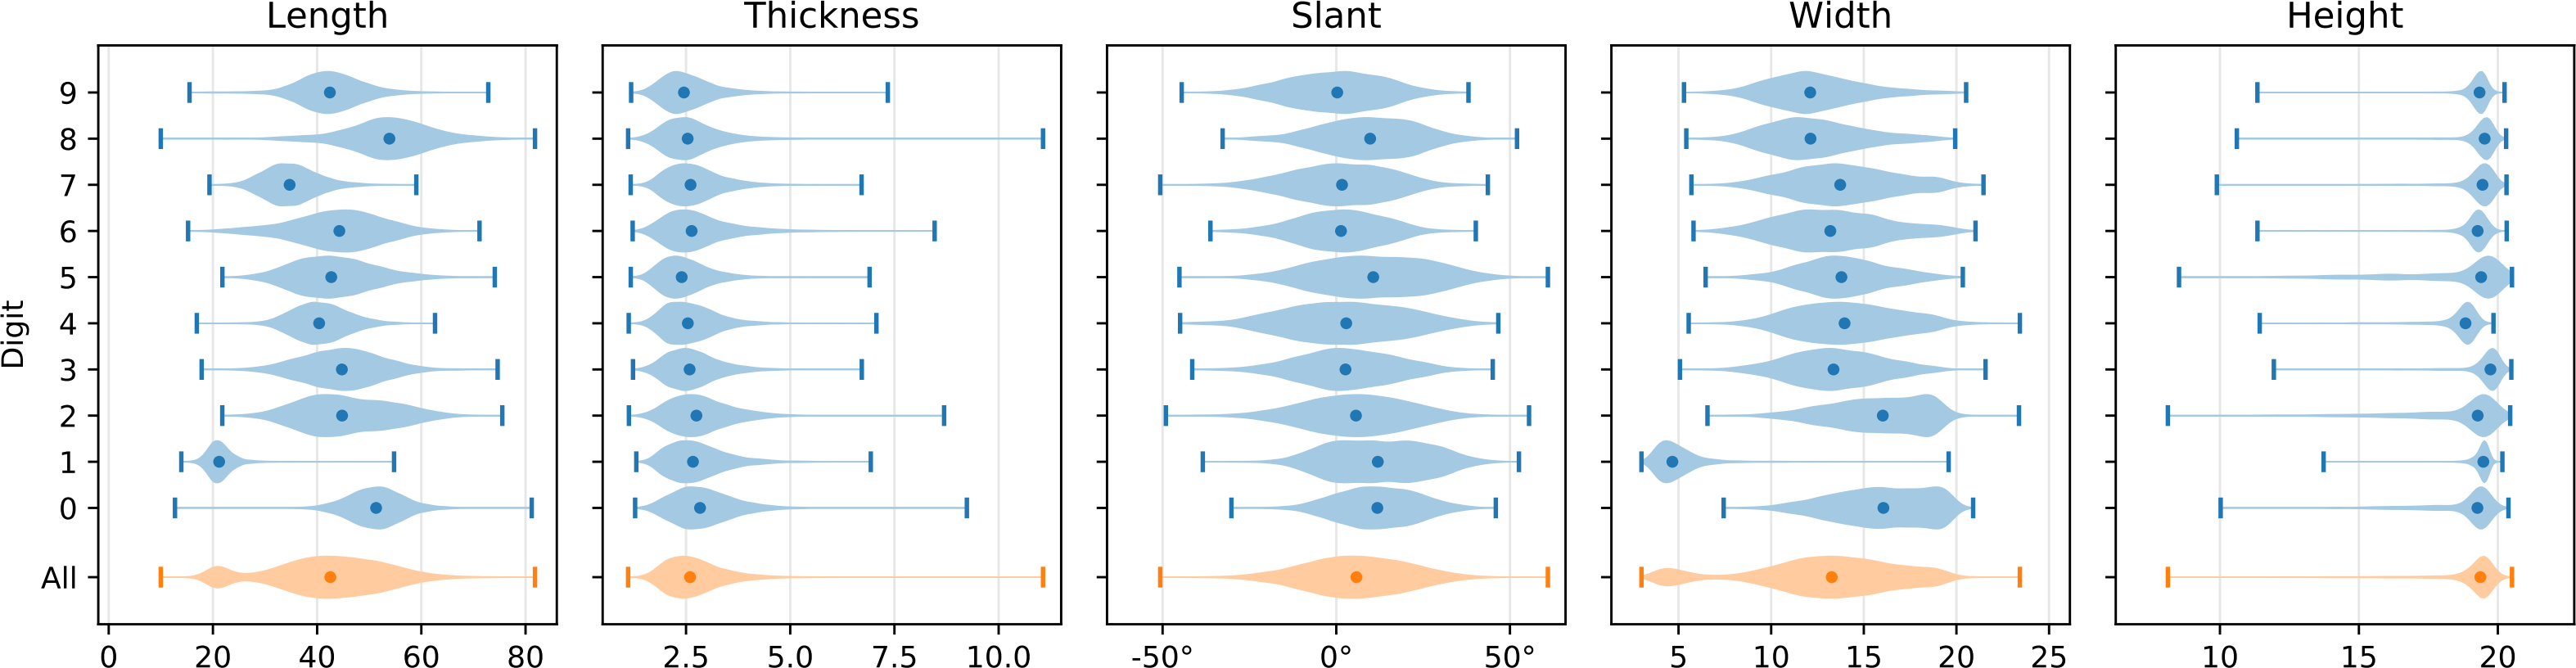
\includegraphics[width=\textwidth]{images/morpho_mnist_distribution.png}
    \caption[Morpho-\textsc{Mnist} distribution]{Distribution of the Morpho-\textsc{Mnist} attributes for the different digits. Taken from~\citep{castro2019morpho}.}
    \label{fig:morpho_mnist_distribution}
\end{figure}

Morpho-\textsc{Mnist}~\citep{castro2019morpho} is an extension of the \textsc{Mnist} dataset that addresses the question: \say{[T]o what extent has my model learned to represent specific factors of
variation in the data?} ~\citep{castro2019morpho}.
To address this questions, Morpho-\textsc{Mnist} provides the following (continuous) labels of morphological attributes of the \textsc{Mnist} samples: stroke length, stroke thickness, slant, width, and height.

Besides providing additional labels of low-level \textsc{Mnist} attributes, Morpho-\textsc{Mnist} provides a toolbox to measure (i.e~ calculate the morphological labels) and perturb MNIST images.
The perturbation toolbox allows it to thin, thicken, swell, and to add fractures to an image.
Morpho-\textsc{Mnist} also provides pre-computed datasets that were built using the perturbation toolbox.

Importantly, the distribution of the morphological attributes partly is highly skewed (for example Thickness and Height, see Figure~\ref{fig:morpho_mnist_distribution}).

\subsubsection{dSprites}
dSprites\footnote{\href{https://github.com/deepmind/dsprites-dataset/}{https://github.com/deepmind/dsprites-dataset/}, last access: 5/28/2020}~\citep{dsprites17} is a dataset designed \say{to assess the disentanglement properties of unsupervised learning methods.}.
It contains 737,280 grayscale images of size $64\times 64$ pixels.
The images were generated from \say{6 ground truth independent latent factors}: color, shape, scale, orientation, $x$-position, and $y$-position.
The color is white in all images.
The shapes are: square, ellipse, and heart.
For the other factors, points are chosen evenly along their support: six values in $[0.5, 1]$ (scale), 40 values in $[0, 2\pi]$ (orientation), 32 values in $[0, 1]$ ($x$-position and $y$-position).
Each factor combination only occurs once in the data set.
The dataset also contains the factor labels for each image.

\subsection{Models}\label{subsec:models}

Four different base \ac{VAE} models were evaluated in the course of this thesis.
Furthermore, two \say{AlexNet} models were used for some additional experiments.

The models vary depending on the dataset and are described in the following.
A more detailed description can be found in Appendix~\ref{sec:appendix_network_architectures}.

\subsubsection{VAE Models}\label{subsubsec:vae_models}

\begin{figure}
    \centering
    \begin{subfigure}{.5\textwidth}
        \centering
        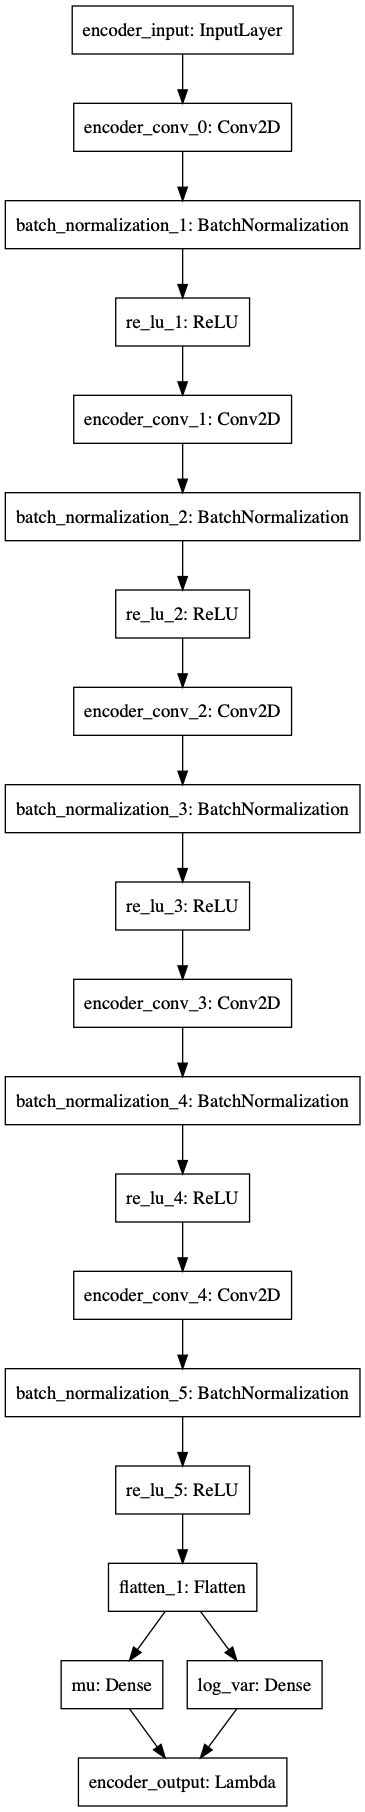
\includegraphics[width=\textwidth,height=.85\textheight,keepaspectratio]{images/vae/encoder.png}
        \caption{Encoder}
    \end{subfigure}%
    \begin{subfigure}{.5\textwidth}
        \centering
        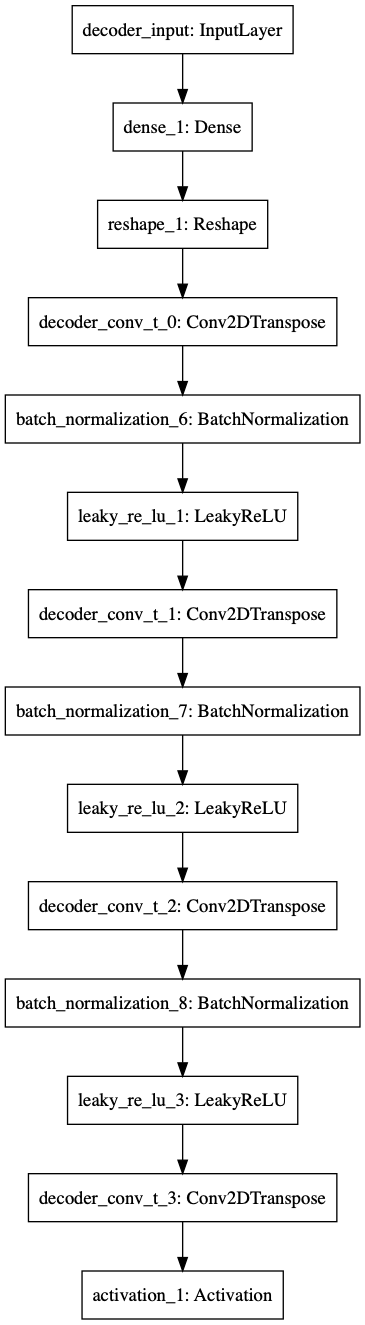
\includegraphics[width=\textwidth,height=.85\textheight,keepaspectratio]{images/vae/decoder.png}
        \caption{Decoder}
    \end{subfigure}
    \caption{\ac{VAE} model structure}
    \label{fig:vae_model_structure}
\end{figure}

The \ac{VAE} model (see Section-\ref{fig:vae_model_structure}) consists of an encoder and a decoder.
The encoder is made up of multiple \say{Convolution, Activation, Batch-Normalization}-blocks, followed by the embedding layer.
The embedding layer predicts $\mu$ and $\log \sigma^2$ and performs the resampling by:
\begin{align}
    z &= \mu + \epsilon\sigma \\
    \epsilon &\sim \mathcal{N}(0, \bm{I}). \label{eq:resampling_vae}
\end{align}
The encoder input size is equal to the decoder output size and is depending on the dataset.
The number of \say{Convolution, Activation, Batch-Normalization}-blocks is chosen depending on the input size, as smaller input sizes require fewer layers to achieve a receptive field of the input size.
The batch-normalization~~\citep[pp. 317, ff.]{Goodfellow-et-al-2016} can be omitted\footnote{It is stated in the experiments if batch-normalization is omitted.}.
The activation can be either ReLU~\citep[p. 173]{Goodfellow-et-al-2016} or LeakyReLU~\citep[p. 192]{Goodfellow-et-al-2016} and is ReLU unless stated otherwise.
The convolutions use zero-padding unless stated otherwise.
Encoder and decoder use stridden convolutions for downsampling, unless stated otherwise.

The \ac{VAE} model implements the loss function from Equation~\ref{eq:elbo_error_term} but with a pre-factor for the reconstruction term.
The reconstruction term pre-factor was determined empirically, observing reconstruction and generation quality.

The decoder uses similar blocks as the encoder but employs transposed convolutions~\citep[pp. 356, ff.]{Goodfellow-et-al-2016} instead of convolutions to upsample feature maps.
The output layer of the decoder uses a sigmoid activation instead of ReLU.

In total, eight \ac{VAE}-models are used: \say{\textsc{Mnist}-\ac{VAE}}, \say{dsprites-\ac{VAE}}, \say{7,500-\ac{VAE}}, \say{6,250-\ac{VAE}}, \say{5,000-\ac{VAE}},  \say{3,750-\ac{VAE}}, \say{dsprites-\ac{VAE}-dim6}, and \say{CelebA-\ac{VAE}}.
The model structures can be found in Appendix~\ref{subseq:appendix_vae_models}.

\paragraph{\textsc{Mnist}-\ac{VAE}} \textsc{Mnist}-\ac{VAE} uses an input- and output-size of $28\times 28\times 1$ (\textsc{Mnist} images are grayscale images).
The model is trained with the Adam optimizer on the \textsc{Mnist} training set with a batch size of 128 and a learning rate of 0.001 for 200 epochs.
The reconstruction loss factor is 10,000.
The latent space is two-dimensional.
The inner activation function is ReLU.

\paragraph{dSprites-\ac{VAE}} dSprites-\ac{VAE} uses an input- and output-size of $64\times 64\times 1$.
The model is trained with the Adam optimizer on a training set consisting of 90\% of the dSprites dataset with a batch size of 128 and a learning rate of 0.001 for 200 epochs.
The reconstruction loss factor is 10,000.
The latent space is ten-dimensional.
The inner activation function is ReLU.
For dSprites, four additional models have been trained with a different reconstruction term weight: 7,500-\ac{VAE}, 6,250-\ac{VAE}, 5,000-\ac{VAE}, and 3,750-\ac{VAE}.
These models differ from dSprites-\ac{VAE} only in the reconstruction term weight.

\paragraph{dsprites-\ac{VAE}-dim6}
The dsprites-\ac{VAE}-dim6 is equivalent to the dSprites-\ac{VAE} model but uses a six-dimensional latent space.

\paragraph{CelebA-\ac{VAE}} CelebA-\ac{VAE} uses an input- and output-size of $128\times 128\times 3$.
The model is trained with the Adam optimizer on a training set consisting of 90\% of the CelebA dataset with a batch size of 128 and a learning rate of 0.001 for 200 epochs.
The reconstruction loss factor is 10,000.
The latent space is eight-dimensional.
The inner activation function is ReLU.

\subsubsection{VLAE Models}\label{subsubsec:vlae_models}
\begin{figure}
    \centering
    \begin{subfigure}{.5\textwidth}
        \centering
        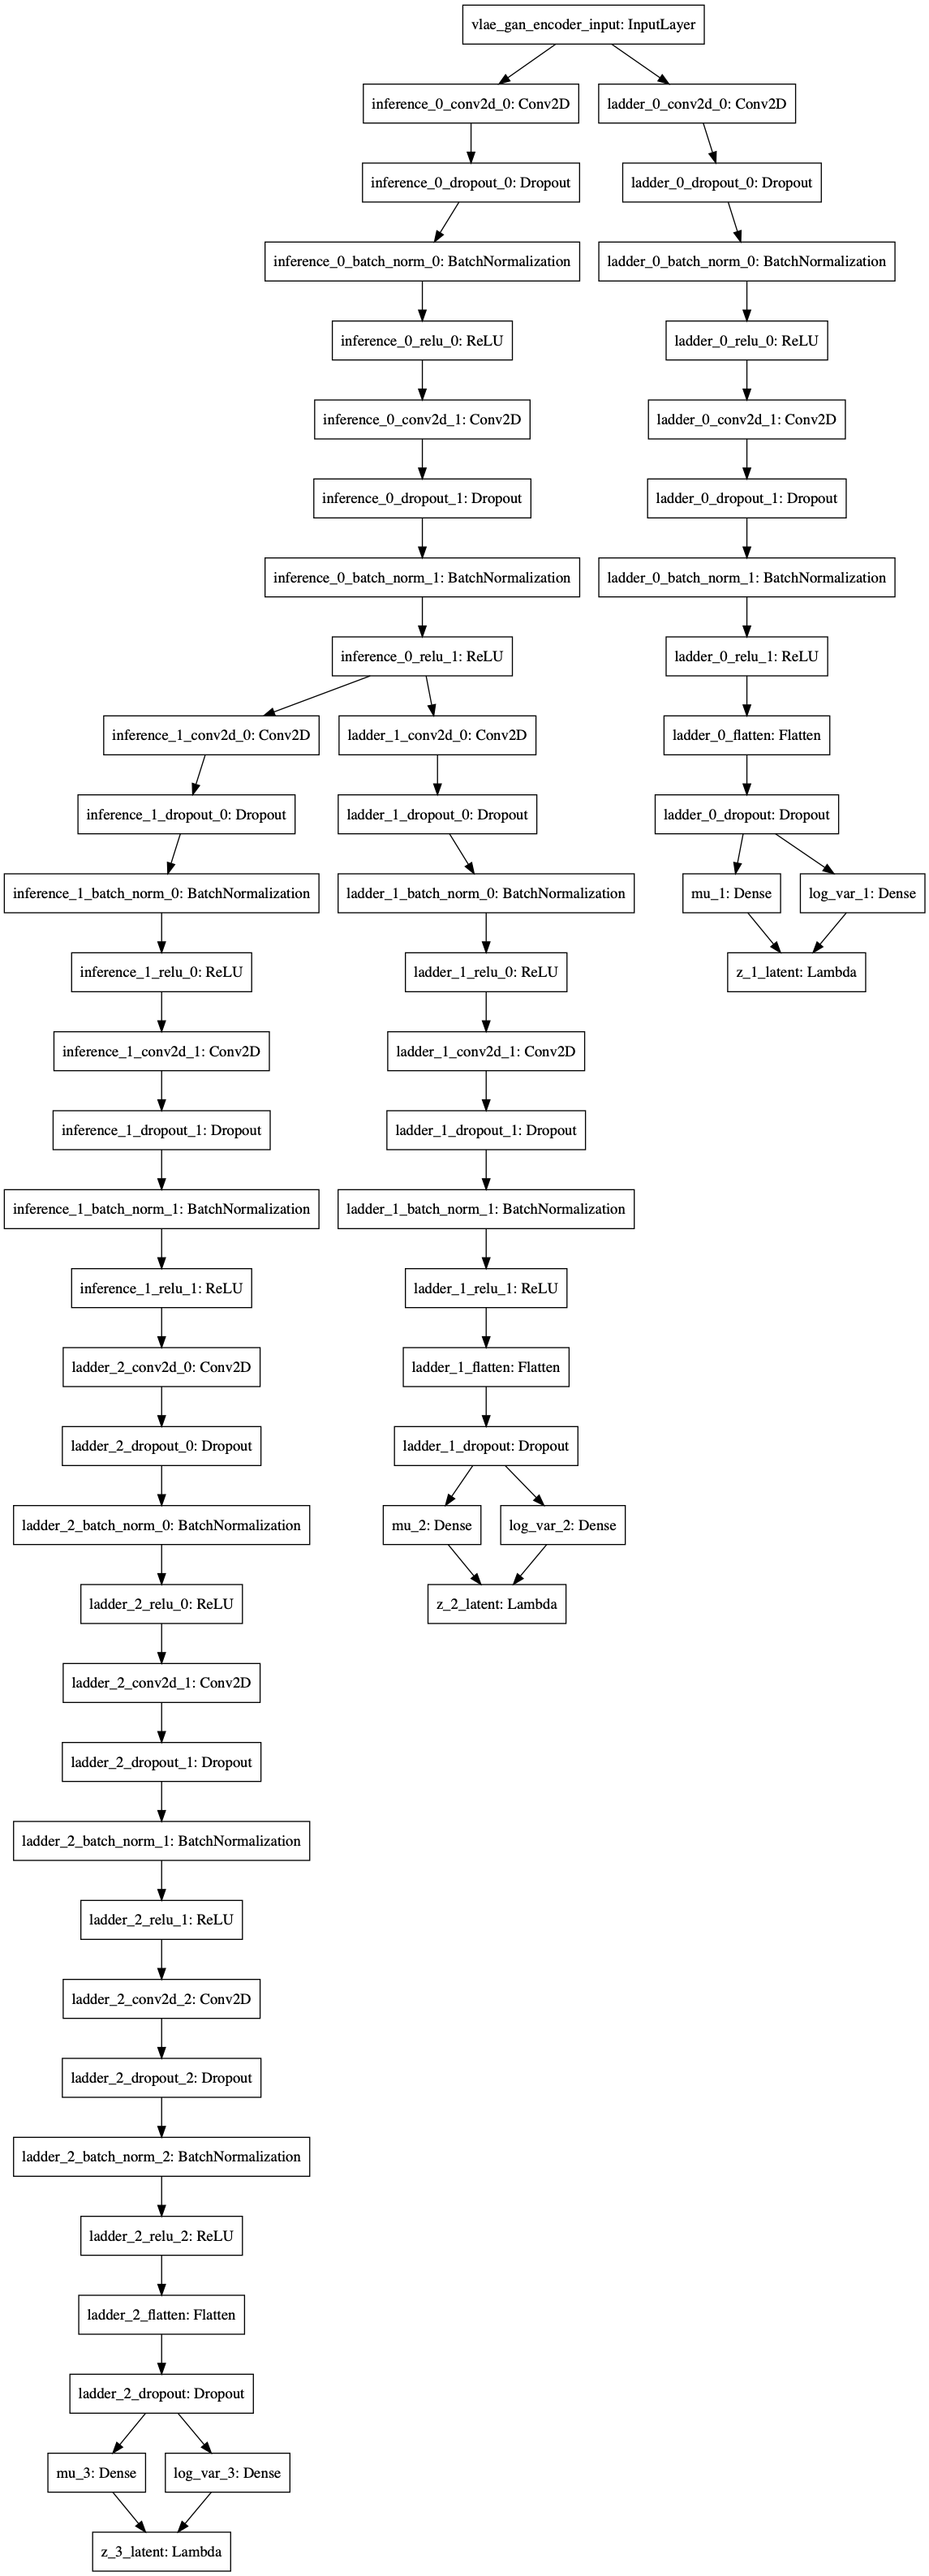
\includegraphics[width=\textwidth,height=.85\textheight,keepaspectratio]{images/vlae/encoder.png}
        \caption{Encoder}
        \label{subfig:vlae_encoder}
    \end{subfigure}%
    \begin{subfigure}{.5\textwidth}
        \centering
        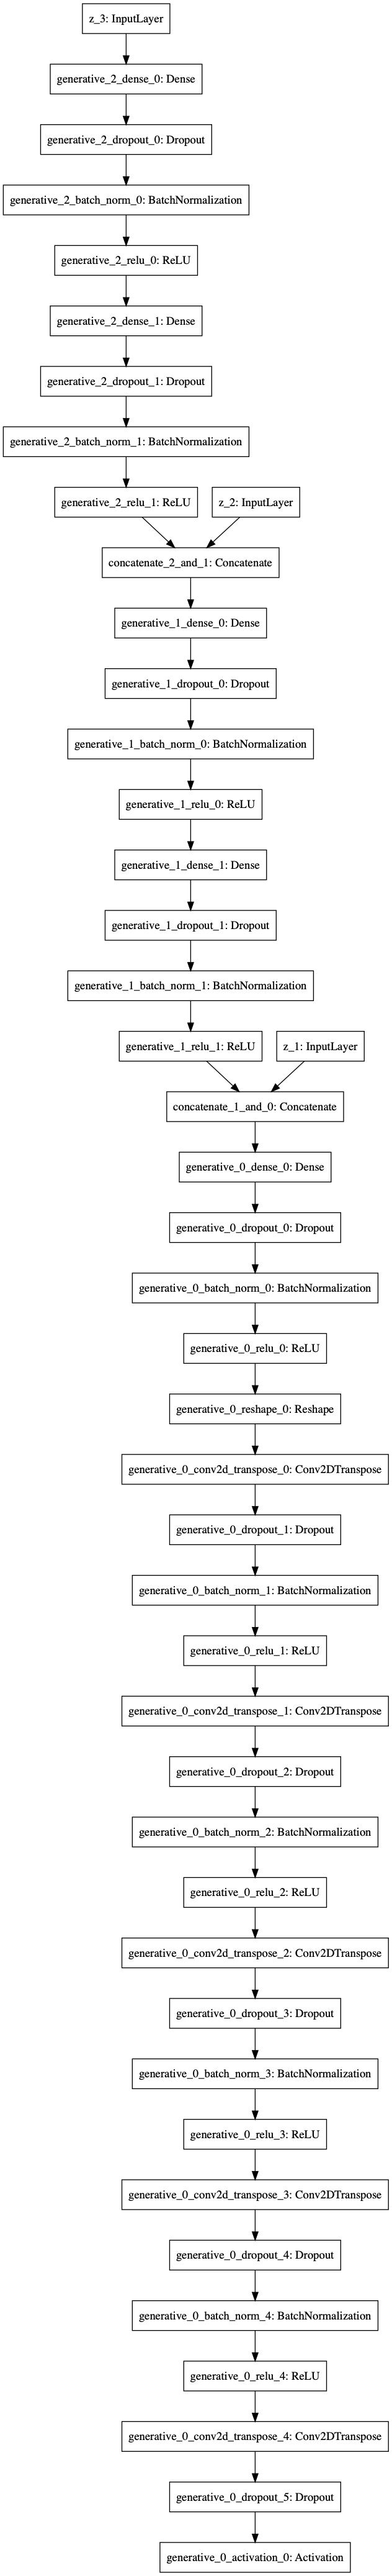
\includegraphics[width=\textwidth,height=.85\textheight,keepaspectratio]{images/vlae/decoder.png}
        \caption{Decoder}
        \label{subfig:vlae_decoder}
    \end{subfigure}
    \caption{\ac{VLAE} model structure}
    \label{fig:vlae_model_structure}
\end{figure}

Figure~\ref{fig:vlae_model_structure} shows the \ac{VLAE} model structure.
Like the \ac{VAE}, it consists of an encoder and a decoder.
The encoder has three latent spaces\footnote{\textit{z\_1\_latent}, \textit{z\_2\_latent}, and \textit{z\_3\_latent} in Figure~\ref{subfig:vlae_encoder}.}
A re-sampling according to Equation~\ref{eq:resampling_vae} is performed for each of the latent spaces.
Lower latent spaces are equipped with a less powerful encoder (e.g., \textit{z\_1\_latent} in Figure~\ref{subfig:vlae_encoder}), higher latent spaces with a more powerful encoder.
Again, the network is composed of multiple \say{Convolution, Activation, Batch-Normalization}-blocks.
The number of these blocks is variable and chosen depending on the dataset.
Batch-normalization can be omitted (default), the inner activation can be either ReLU (default) or LeakyReLU.
The convolutions use-zero padding, and encoder and decoder use stridden convolutions for downsampling.

The \ac{VAE} model implements the loss function from Equation~\ref{eq:elbo_error_term} but with a pre-factor for the reconstruction term.
The \ac{KL}-terms of different layers are totalized.

The decoder has three inputs, where the first input of the decoder\footnote{\textit{z\_3} in Figure~\ref{subfig:vlae_decoder}} receives input from the last output of the encoder\footnote{\textit{z\_3\_latent} in Figure~\ref{subfig:vlae_encoder}}.
The decoder uses blocks similar to the encoder but with transposed convolutions instead of regular convolutions.

In total, six \ac{VLAE}-models are used: \say{\textsc{Mnist}-\ac{VLAE}-factor-1}, \say{\textsc{Mnist}-\ac{VLAE}-factor-2}, \say{\textsc{Mnist}-\ac{VLAE}-factor-3} \say{dSprites-\ac{VLAE}}, \say{dSprites-\ac{VLAE}-dim2}, and \say{CelebA-\ac{VLAE}}.
The model structures can be found in Appendix~\ref{subseq:appendix_vlae_models}.

\paragraph{\textsc{Mnist}-\ac{VLAE}} The three \textsc{Mnist}-\ac{VLAE}s\footnote{\say{\textsc{Mnist}-\ac{VLAE}-factor-1}, \say{\textsc{Mnist}-\ac{VLAE}-factor-2}, \say{\textsc{Mnist}-\ac{VLAE}-factor-3}} use an input- and output-size of $28\times 28\times 1$.
The models are trained with the Adam optimizer on the \textsc{Mnist} training set with a batch size of 128 for 200 epochs.
The reconstruction loss factor is 10,000.
The latent spaces are two-dimensional.
The inner activation function is ReLU.
The models use no batch-normalization.
\textsc{Mnist}-\ac{VLAE}-factor-1 is the model with the original number of feature maps, for \textsc{Mnist}-\ac{VLAE}-factor-2 and \textsc{Mnist}-\ac{VLAE}-factor-3, the number of feature maps is reduced according to the factor.
\textsc{Mnist}-\ac{VLAE}-factor-1 is trained with a learning rate of 0.005.
\textsc{Mnist}-\ac{VLAE}-factor-2 and \textsc{Mnist}-\ac{VLAE}-factor-3 are trained with a learning rate of 0.001.

\paragraph{dSprites-\ac{VLAE}} dSprites-\ac{VLAE} uses an input- and output-size of $64\times 64\times 1$.
The model is trained with the Adam optimizer on a training set consisting of 90\% of the dSprites dataset with a batch size of 128 and a learning rate of 0.001 for 200 epochs.
The reconstruction loss factor is 10,000.
The latent spaces are four-dimensional.
The inner activation function is ReLU.

\paragraph{dSprites-\ac{VLAE}-dim2}
The dSprites-\ac{VLAE}-dim2 model is equivalent to dSprites-\ac{VLAE} but uses a two-dimensional latent space.

\paragraph{CelebA-\ac{VLAE}} CelebA-\ac{VLAE} uses an input- and output-size of $128\times 128\times 3$.
The model is trained with the Adam optimizer on a training set consisting of 90\% of the CelebA dataset with a batch size of 128, a learning rate of 0.001 with an additional learning rate decay of 0.01 for 200 epochs.
The reconstruction loss factor is 10,000.
The latent spaces are two-dimensional.
The inner activation function is ReLU.

\subsubsection{VAE-GAN Models}\label{subsubsec:vae_gan_models}

The \ac{VAE}-\ac{GAN}-model is similar to the \ac{VAE}-model.
However, it implements the \ac{VAE}-\ac{GAN} loss function (see Section~\ref{subsubsec:representation_learning}) instead of Equation~\ref{eq:elbo_error_term}.
Therefore, the \ac{VAE}-\ac{GAN} has an additional \textit{discriminator} network.
The feature loss compares inner activations in the discriminator of true and generated samples.
The discriminator loss signifies by how much the discriminator violates the \ac{GAN} training objective.
See Section~\ref{subsubsec:representation_learning} for more details.

For the encoder, the \ac{KL}-term is weighted ten-times more strongly than the feature loss.
The decoder weights the discriminator loss with factor 1 and the feature loss with factor 0.75.

In total, seven \ac{VAE}-\ac{GAN}-models are used: \say{\textsc{Mnist}-\ac{VAE}-\ac{GAN}}, \say{dSprites-\ac{VAE}-\ac{GAN}}, and \say{CelebA-\ac{VAE}-\ac{GAN}}.
The model structures can be found in Appendix~\ref{subseq:appendix_vae_gan_models}.

\paragraph{\textsc{Mnist}-\ac{VAE}-\ac{GAN}} \textsc{Mnist}-\ac{VAE}-\ac{GAN} uses an input- and output-size of $28\times 28\times 1$.
The model is trained with the Adam optimizer on the \textsc{Mnist} training set with a batch size of 128 and a learning rate of 0.0001 for 200 epochs.
The reconstruction loss factor is 10,000.
The latent space is two-dimensional.
The inner activation function is ReLU.

\paragraph{dSprites-\ac{VAE}-\ac{GAN}} dSprites-\ac{GAN} uses an input- and output-size of $64\times 64\times 1$.
The model is trained with the Adam optimizer on a training set consisting of 90\% of the dSprites dataset with a batch size of 128 and a learning rate of 0.0001 for 200 epochs.
The reconstruction loss factor is 10,000.
The latent space is ten-dimensional.
The inner activation function is ReLU.

\paragraph{CelebA-\ac{VAE}-\ac{GAN}} CelebA-\ac{VAE}-\ac{GAN} uses an input- and output-size of $128\times 128\times 3$.
The model is trained with the Adam optimizer on a training set consisting of 90\% of the CelebA dataset with a batch size of 128 and a learning rate of 0.001 with an additional learning rate decay of 0.02 for 200 epochs.
The reconstruction loss factor is 10,000.
The latent space is eight-dimensional.
The inner activation function is ReLU.

\subsubsection{VLAE-GAN Models}\label{subsubsec:vlae_gan_models}

The \ac{VLAE}-\ac{GAN}-model is comparable to the \ac{VAE}-\ac{GAN}-model in terms of the loss functions.
However, it uses the structure of the \ac{VLAE}-model and totalizes the three $KL$-losses from the different layers.

The model structures can be found in Appendix~\ref{subseq:appendix_vlae_gan_models}.

\paragraph{\textsc{Mnist}-\ac{VLAE}-\ac{GAN}} The three \textsc{Mnist}-\ac{VLAE}-\ac{GAN} uses an input- and output-size of $28\times 28\times 1$.
The model is trained with the Adam optimizer on the \textsc{Mnist} training set with a batch size of 128 and a learning rate of 0.0001 for 200 epochs.
The reconstruction loss factor is 10,000.
The latent spaces are two-dimensional.
The inner activation function is ReLU.
The model uses no batch-normalization.

\paragraph{dSprites-\ac{VLAE}-\ac{GAN}} dSprites-\ac{VLAE}-\ac{GAN} uses an input- and output-size of $64\times 64\times 1$.
The model is trained with the Adam optimizer on a training set consisting of 90\% of the dSprites dataset with a batch size of 128, a learning rate of 0.0001, and an additional learning rate decay of 0.01 for 200 epochs.
The reconstruction loss factor is 10,000.
The latent spaces are four-dimensional.
The inner activation function is ReLU.

\paragraph{CelebA-\ac{VLAE}-\ac{GAN}} CelebA-\ac{VLAE}-\ac{GAN} uses an input- and output-size of $128\times 128\times 3$.
The model is trained with the Adam optimizer on a training set consisting of 90\% of the CelebA dataset with a batch size of 128, a learning rate of 0.0001 with an additional learning rate decay of 0.01 for 200 epochs.
The reconstruction loss factor is 10,000.
The latent spaces are two-dimensional.
The inner activation function is ReLU.

\subsubsection{AlexNet Classifier}\label{subsubsec:alexnet_classifier}
The AlexNet Classifier resembles the architecture from \citet{krizhevsky2012imagenet}.
It uses dropout and a dropout rate of 0.3.
The model is trained with the Adam optimizer and a learning rate of 0.0001 using batch normalization and a batch size of 32 for ten epochs..
The model structure can be found in Appendix~\ref{subseq:appendix_alexnet_classifiers}.

\subsubsection{AlexNet-\ac{VAE}}\label{subsubsec:alexnet_vae}
The AlexNet-\ac{VAE} resembles the AlexNet classifier but uses a 2000-dimensional latent space with re-sampling (see Equation~\ref{eq:resampling_vae}).
For AlexNet-\ac{VAE}, no dropout is used.
The model is trained with the Adam optimizer and a learning rate of 0.0001 using batch normalization and a batch size of 32 for 100 epochs..
The model structure can be found in Appendix~\ref{subseq:appendix_alexnet_vae}.


\section{Results and Discussion}\label{sec:results}
\subsection{Visual Features in Variational Autoencoders}\label{subsec:results_visual_features_in_variational_autoencoders}
The following sections describe the results of the experiments on visual features in variational autoencoders.

\begin{itemize}
    \item Results non-AlexNet-like-VAE on CelebA: especially layer 1 kernels
    \item Results AlexNet-like-VAE on ImageNet: especially layer 1 kernels
    \item Results AlexNet-like image classification CNN on ImageNet: especially layer 1 kernels
    \item Results AlexNet-like-VAE with frozen decoder from classification network
\end{itemize}

\subsubsection{AlexNet Image Classification}
To make sure that the network structure of the \ac{VAE} is apt to generate Gabor wavelets, image classification was performed on ImageNet (see Figure~\ref{fig:alexnet} and Section~\ref{subsec:visual-features-variational-autoencoders} for the used network, see Section~\ref{ssec:imagenet} for ImageNet).
As the accuracy was not of primary concern, the training was stopped during the tenth epoch (\textbf{If time: train all 100 epochs}), the top-1 training accuracy at this time was at 0.85.

\begin{figure}
    \centering
    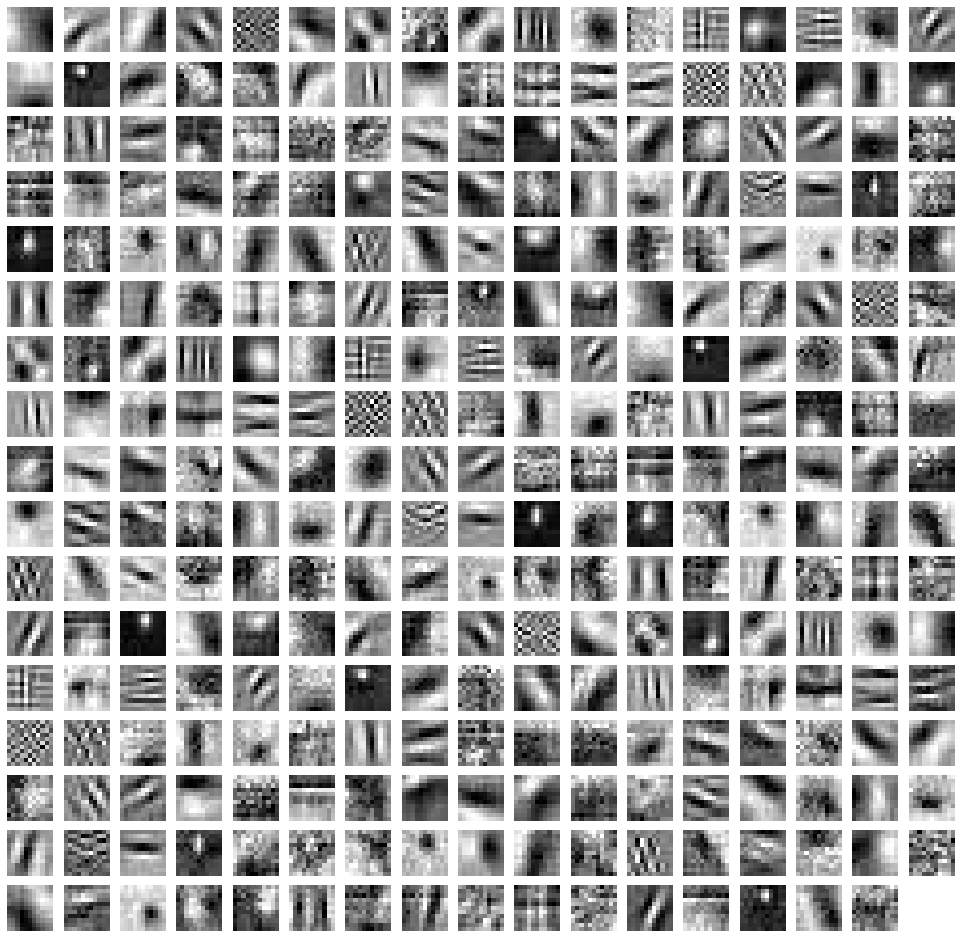
\includegraphics[width=0.9\textwidth]{images/alexnet_classification_l1_kernels.png}
    \caption[Image classification - Layer 1 Kernels]{Convolutional Kernels in the first layer of the image classification network. The filters are shown in their original size (11x11).}
    \label{fig:classification_layer1_kernels}
\end{figure}

Figure~\ref{fig:classification_layer1_kernels} shows all 256 convolutional kernels of the image classification network.
It is easy to see that in many kernels, Gabor wavelet-like filters emerge.

\subsection{V(L)AE Generated Samples vs. True Samples}\label{subsec:vae-generated-samples-vs-true-samples}
\acp{GAN} (see Section~\ref{subsubsec:representation_learning}) are trained by simulatenously training a \textit{generator} to create new samples and a \textit{discriminator} to discriminate between true and generated samples.
\acp{VAE} are another generative model that is not forced in the same way to create indistinguishable samples.
Instead, a reconstruction loss is used to force the reconstruction to be close to the true sample in terms of difference in the pixel values.
At the same time, the \ac{KL}-loss and the reparametrization trick force the model to place similar samples close toanother in a continuous Gaussian embedding space.
Drawing from the Gaussian embedding space therefore should allow to generate new samples similar to true samples.
However, the question remains how indistinguishable these generates samples are from true samples.

To address this question, different statistical analyses were performed revealing that in fact VAE generated samples can be perfectly distinguished from true samples.
\textbf{Talk about the blurriness in VAE generated samples that are another strong reason why this is possible.}

\begin{figure}
    \centering
    \begin{subfigure}{0.4\textwidth}
        \centering
        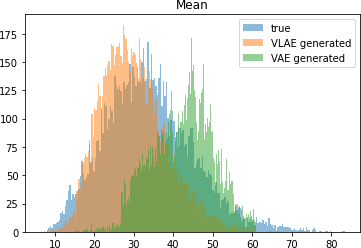
\includegraphics[width=\textwidth]{images/vlae_generated_vs_true/mnist_vs_vlae_mean.png}
        \caption{Mean}
        \label{subfig:vlae_mean_generated_vs_true}
    \end{subfigure}
    \hfill
    \begin{subfigure}{0.4\textwidth}
        \centering
        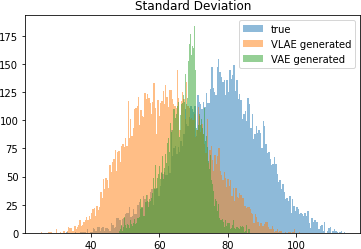
\includegraphics[width=\textwidth]{images/vlae_generated_vs_true/mnist_vs_vlae_sd.png}
        \caption{Standard Deviation}
        \label{subfig:vae_sd_generated_vs_true}
    \end{subfigure}
    \hfill
    \begin{subfigure}{0.4\textwidth}
        \centering
        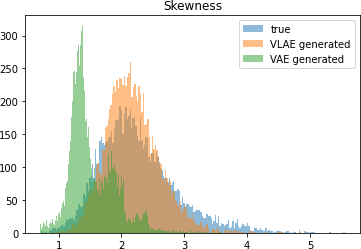
\includegraphics[width=\textwidth]{images/vlae_generated_vs_true/mnist_vs_vlae_skew.png}
        \caption{Skewness}
        \label{subfig:vae_skew_generated_vs_true}
    \end{subfigure}
    \hfill
    \begin{subfigure}{0.4\textwidth}
        \centering
        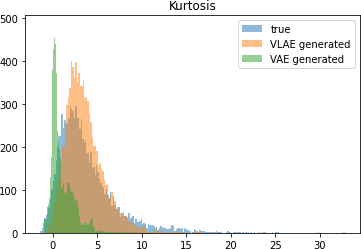
\includegraphics[width=\textwidth]{images/vlae_generated_vs_true/mnist_vs_vlae_kurt.png}
        \caption{Kurtosis}
        \label{subfig:vae_kurt_generated_vs_true}
    \end{subfigure}
    \caption{Comparison of image statistics of \ac{VAE} and \ac{VLAE} compared to \textsc{MNIST} test images. }
    \label{fig:mean_generated_vs_true}
\end{figure}


The MNIST test set of 10,000 images was compared to a 10.000 generated samples from the Vanilla \ac{VAE} and the \ac{VLAE}.
The samples were generated by drawing from a standard two-dimensional Gaussian distribution $\mathcal{N}^2(\bm{0},\bm{I})$.
First, the mean pixel values, i.e.~the mean over all $28\times 28$ pixel values, were compared (see Figure~\ref{subfig:vlae_mean_generated_vs_true}).
The plot overlays the histograms of mean pixel values for the three conditions: \textsc{MNIST}, \ac{VAE}, and \ac{VLAE}.
The other plots in Figure~\ref{fig:mean_generated_vs_true} were created accordingly but for higher moments of the pixel value distributions.

Analyzing Figure~\ref{fig:mean_generated_vs_true} leads to the assumption that, except for Figure~\ref{subfig:vae_sd_generated_vs_true}, the \ac{VLAE} captures the statistics better than the \ac{VAE}.
\begin{table}
    \begin{tabular}{lrrrr}
        \toprule
        Model & $p$-value (mean) & $p$-value (sd) & $p$-value (skewness) & $p$-value (kurtosis)\\
        \midrule
        \ac{VAE} & 0.0 & 0.0 & 0.0 & 0.0 \\
        \ac{VLAE} & $1.8\cdot 10^{-147}$ & 0.0 & $7.9\cdot 10^{-11}$ & 0.309\\
        \bottomrule
    \end{tabular}
    \caption{$p$-values of a Wilcoxon signed-rank test. Each cell tests the hypothesis that the respective moments for the respective model are equal to the values for the \textsc{MNIST} test images. For each cell, the sample size was $2\cdot 10,000$.}
    \label{tab:vae-vlae-mnist}
\end{table}
Table~\ref{tab:vae-vlae-mnist} shows the results of a Wilcoxon signed-rank test for the samples of moments of the pixel distributions.
The results lead to two conclusions: 1) The \ac{VLAE} in fact captures the statistics of the pixel distribution better compared to the \ac{VAE}.
2) Both models do not capture the true pixel distribution.

Similar to the \ac{GAN} approach, a discriminator network was trained to distinguish generated samples from true \textsc{MNIST} test images\footnote{The configuration of the discriminator network can be found in Appendix \ref{sec:listing_discriminator_network}.}.
The discriminator network shows an accuracy of 1.0 for distinguishing both, \ac{VAE} generated from \textsc{MNIST} test images as well as  \ac{VLAE} from \textsc{MNIST} test images.

\subsection{Independence of VLAE Embeddings}\label{subsec:independence-of-vlae-embeddings}

\begin{figure}[t]
    \centering
    \begin{subfigure}{0.3\textwidth}
        \centering
        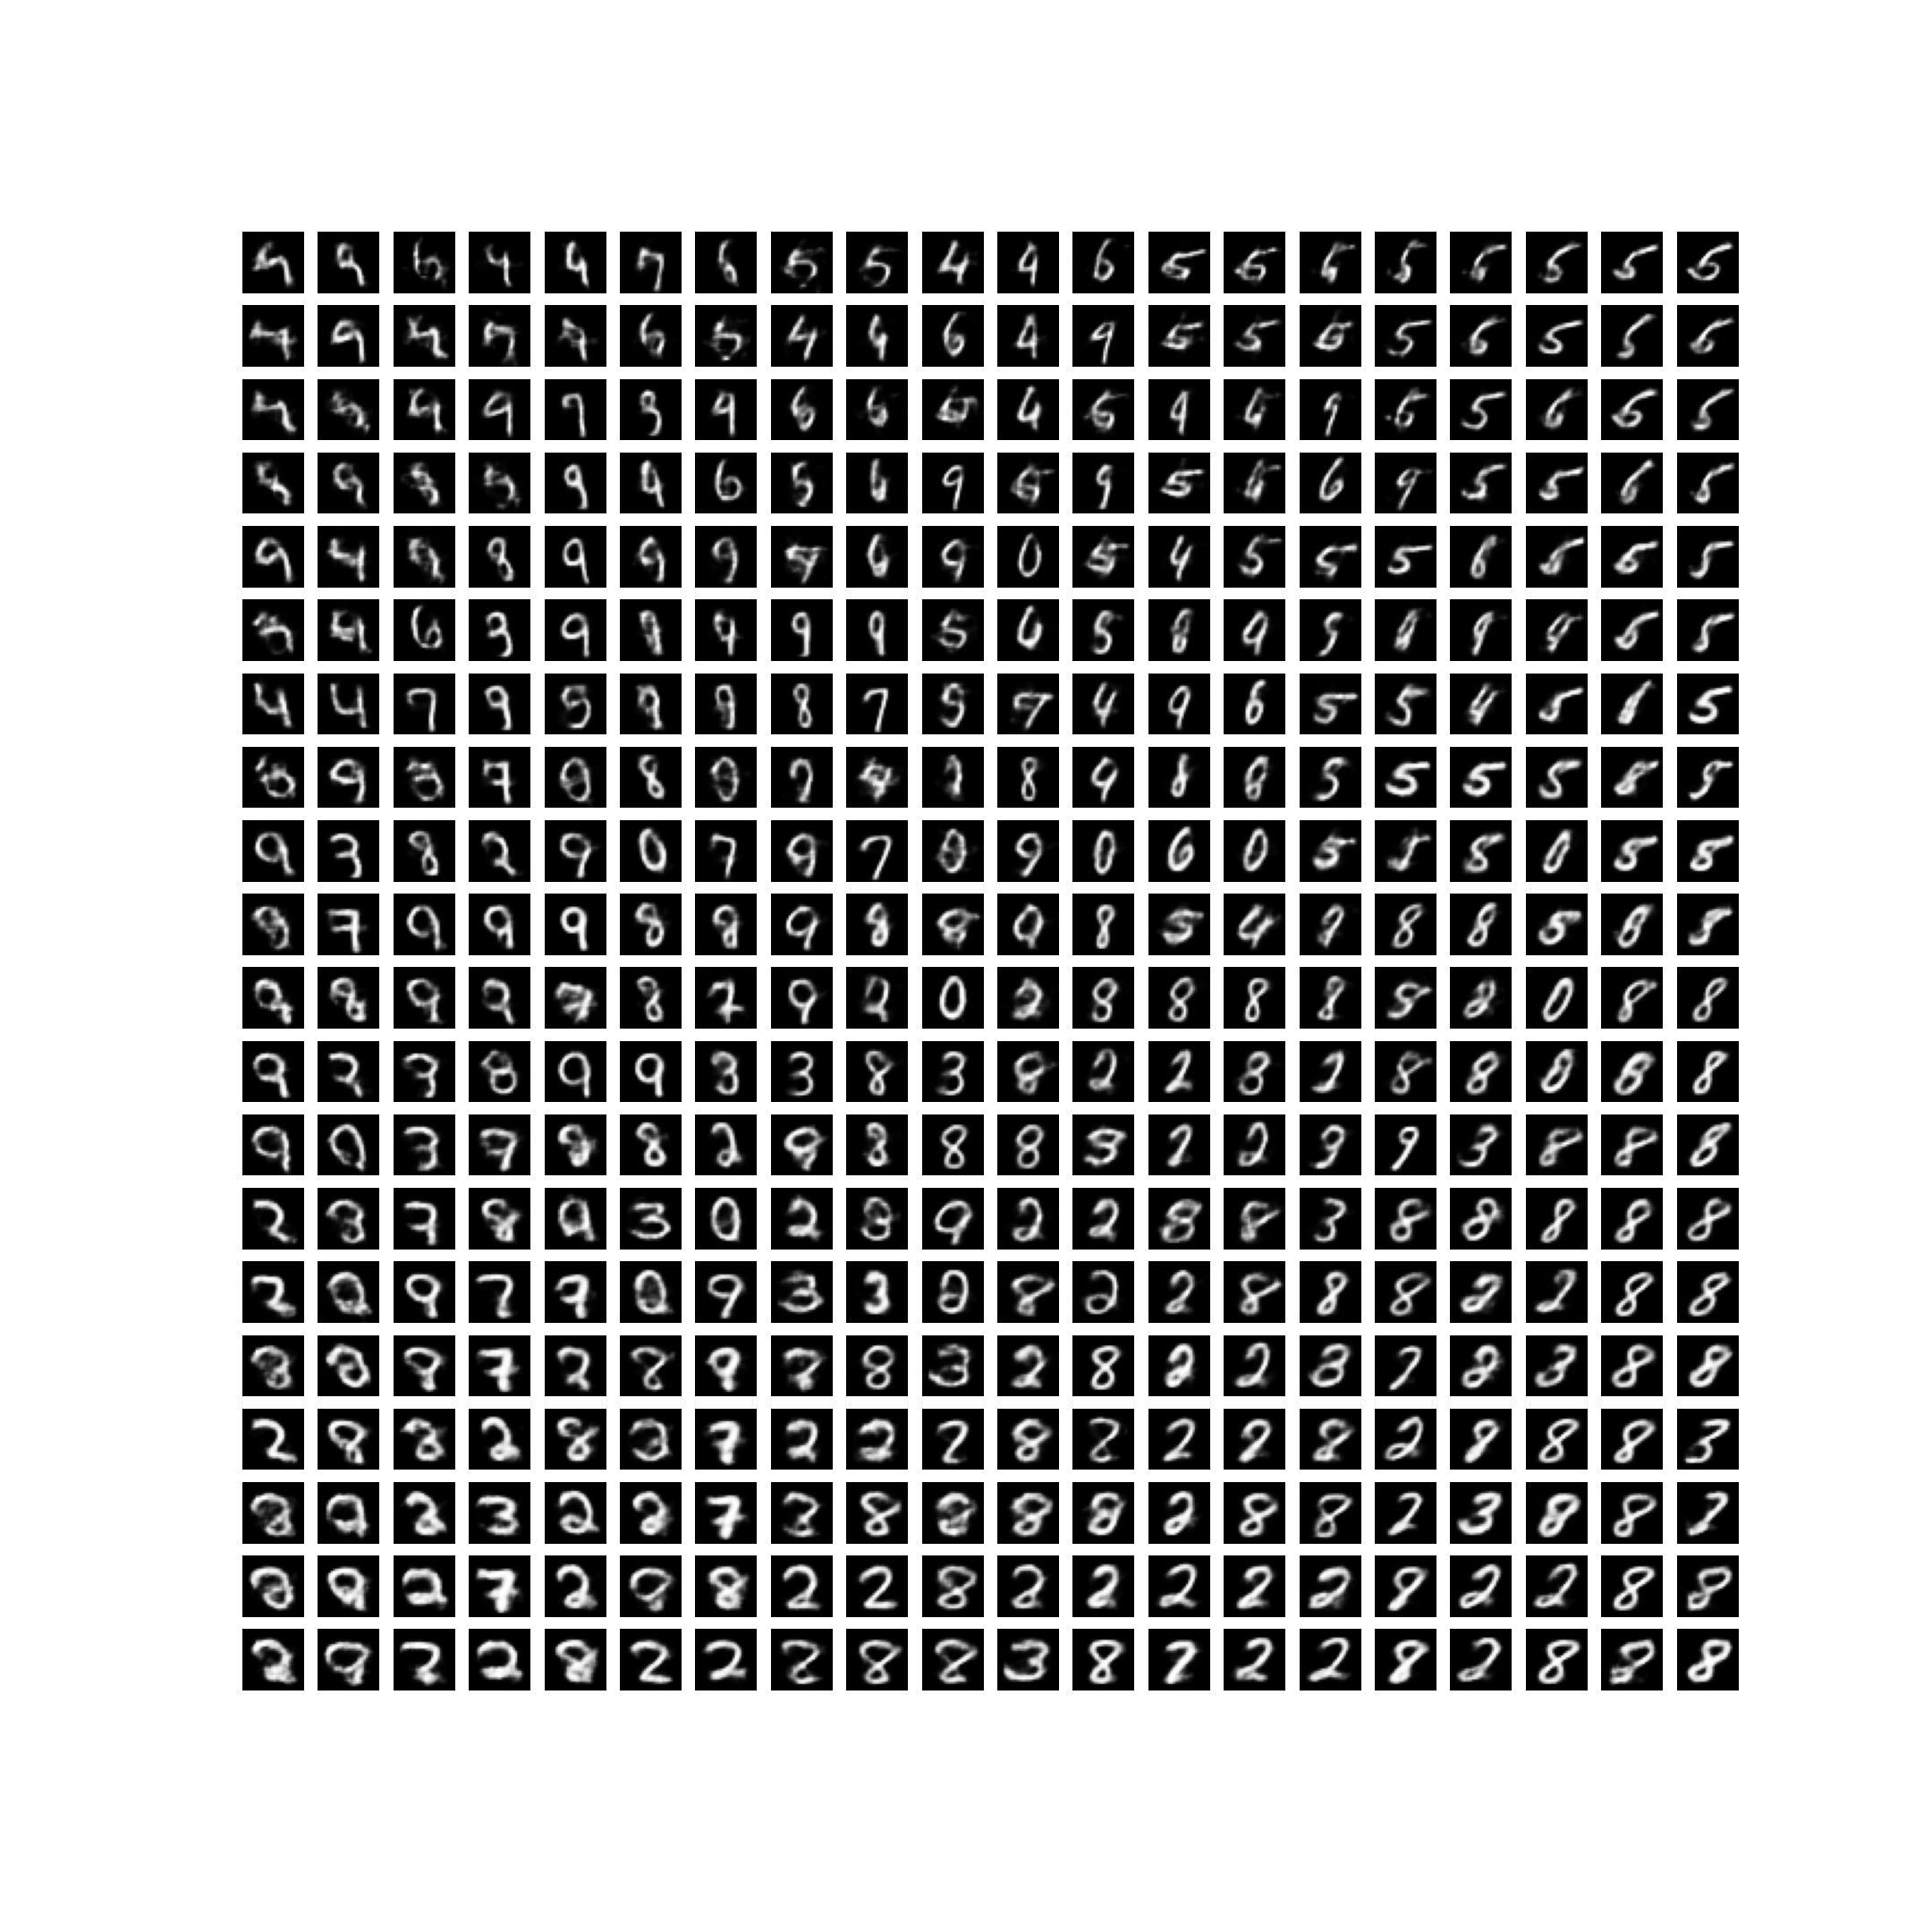
\includegraphics[width=\textwidth]{images/vlae_plots1.png}
        \caption{Exploring $z_1$}
        \label{subfig:vlae_plots1}
    \end{subfigure}
    \hfill
    \begin{subfigure}{0.3\textwidth}
        \centering
        
\includegraphics[width=\textwidth]{images/vlae_plots2.png}
        \caption{Exploring $z_{2}$}
        \label{subfig:vlae_plots2}
    \end{subfigure}
    \hfill
    \begin{subfigure}{0.3\textwidth}
        \centering
        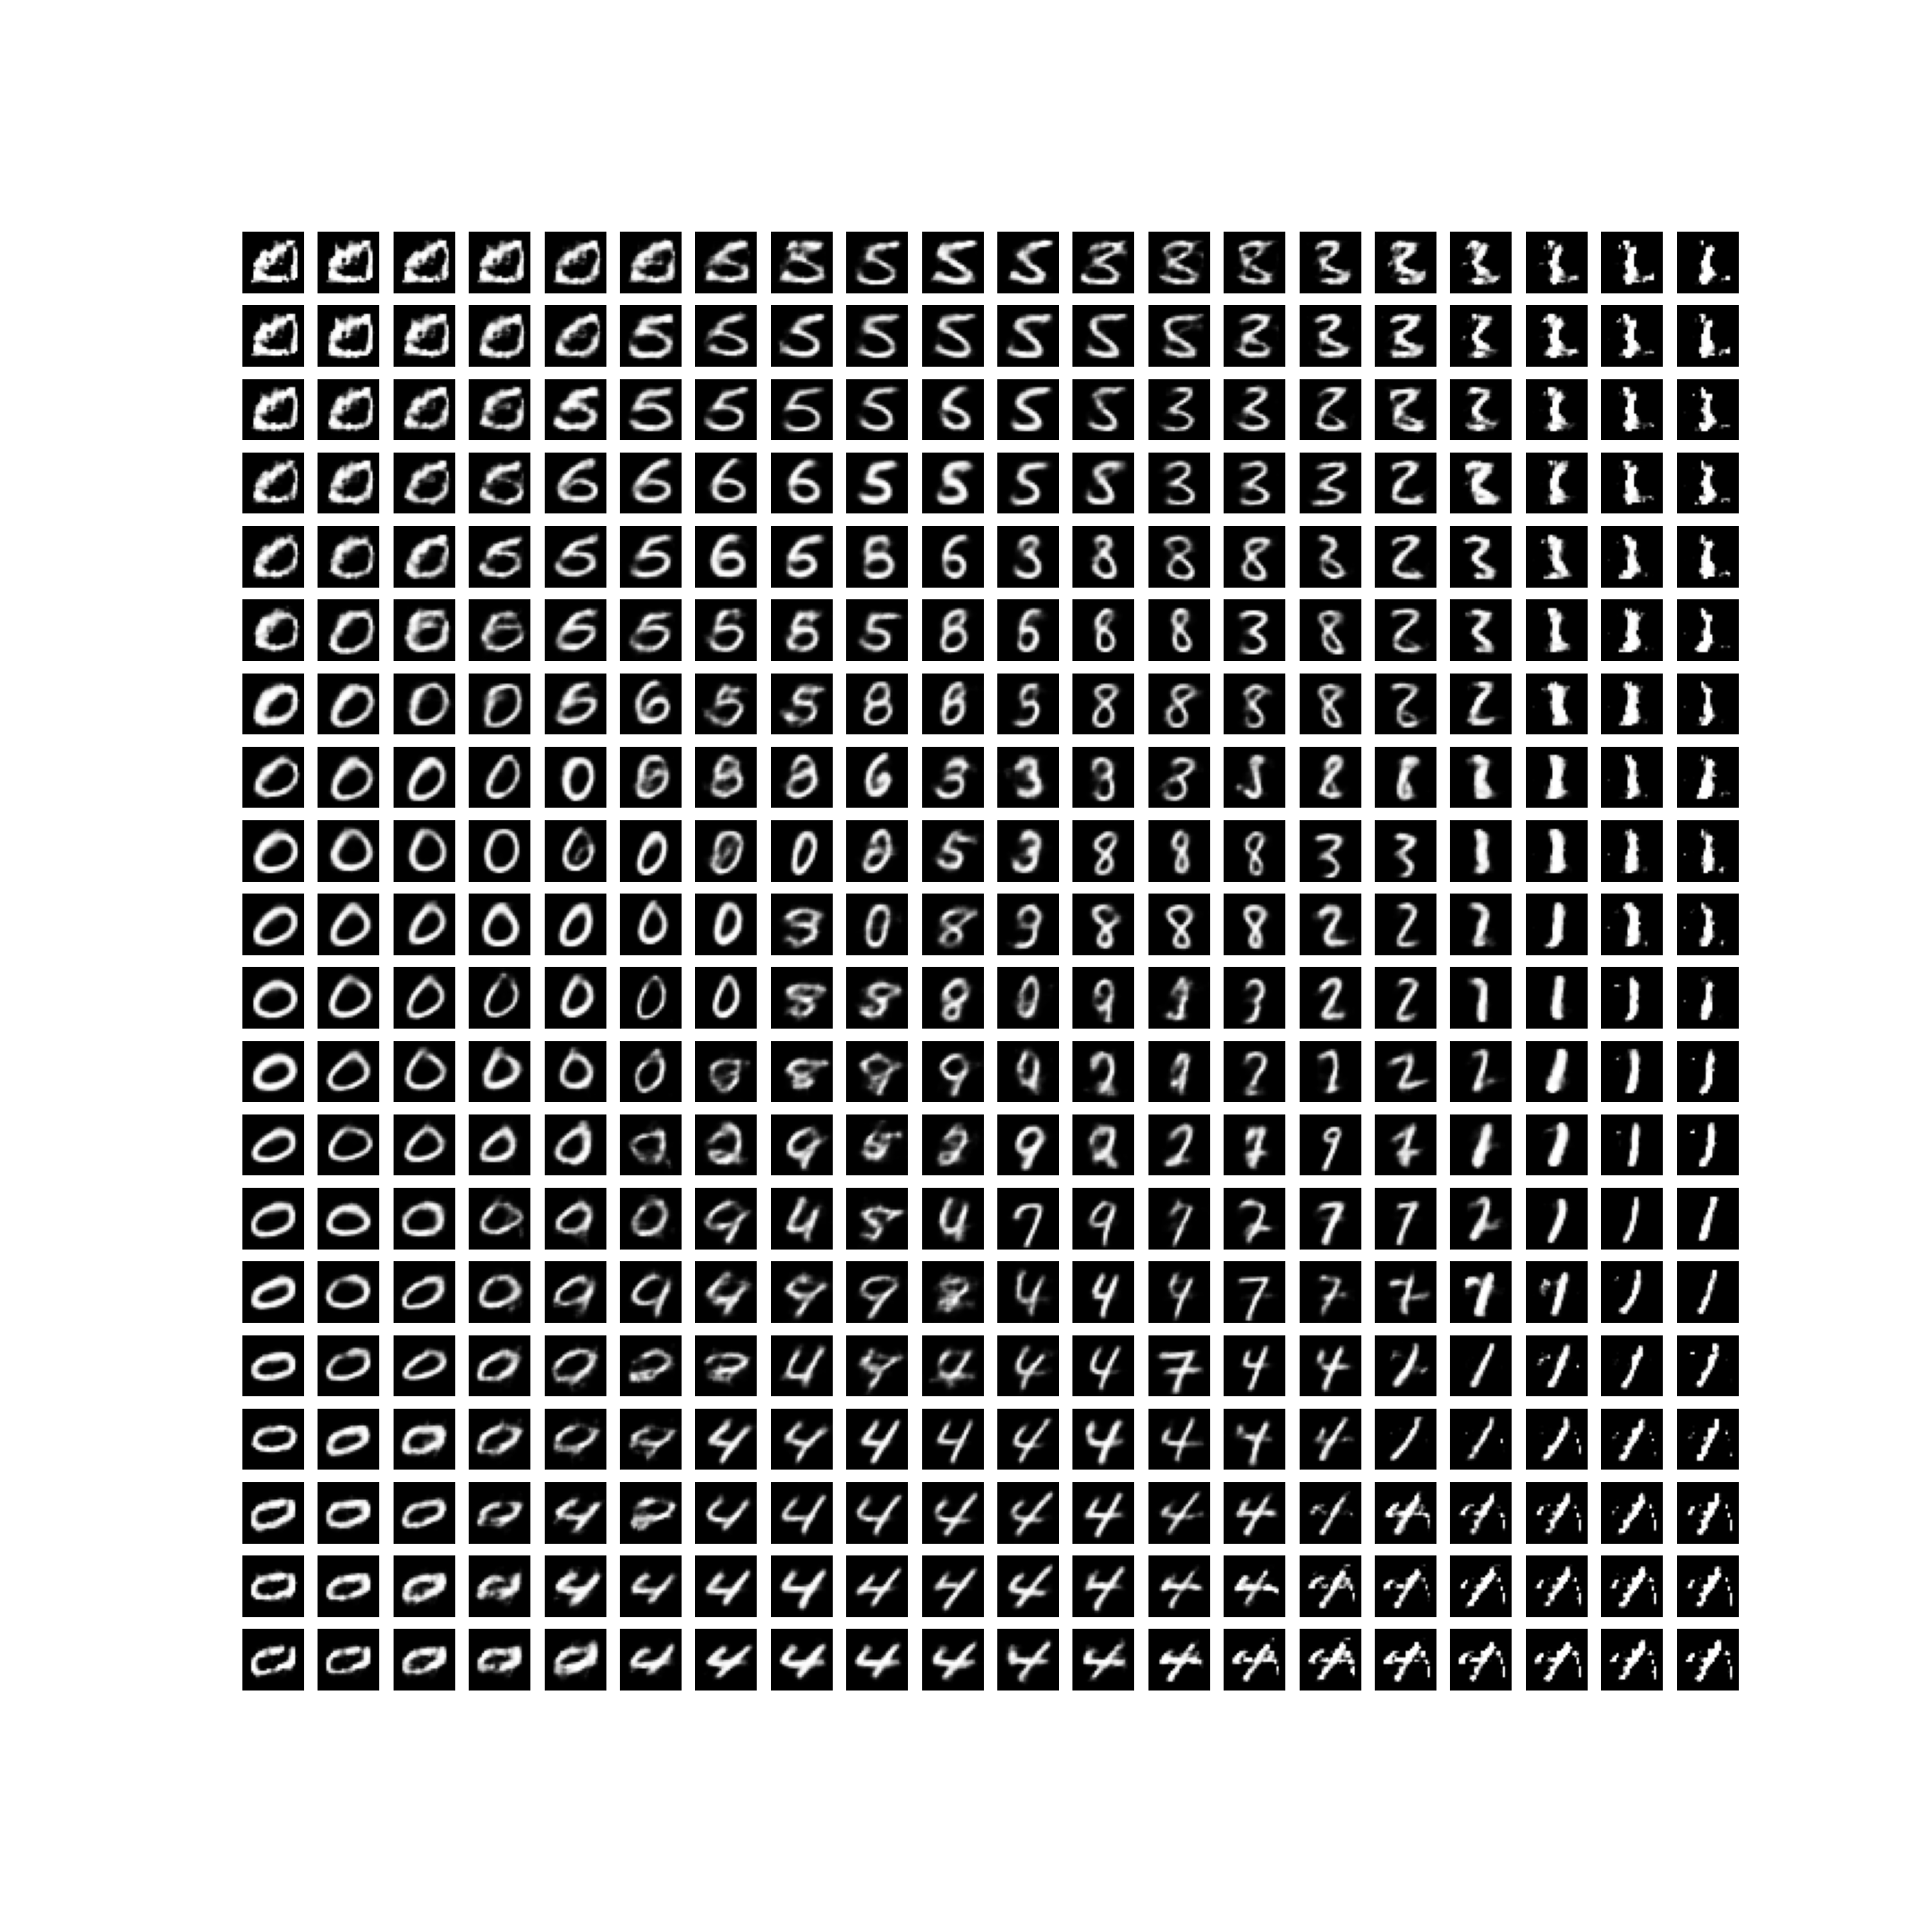
\includegraphics[width=\textwidth]{images/vlae_plots3.png}
        \caption{Exploring $z_3$}
        \label{subfig:vlae_plots3}
    \end{subfigure}
    \caption{Reconstructions of the VLAE model when systematically exploring one latent space and randomly choosing the other two latent spaces. The space explored systematically is sampled from -3 SD to 3 SD in both dimensions, the other values are chosen by drawing from an uniform distribution over $[-1; 1]$. Created analogously to \citet[Figure 5]{zhao2017learning}.}
    \label{fig:vlae_plots}
\end{figure}
The VLAE learns embeddings on different levels.
For MNIST, \citet{zhao2017learning} used three two-dimensional layers to learn image semantics of different granularity.
They claim that their model is able to learn disentangled hierarchical features.
Figure~\ref{fig:vlae_plots} shows reconstructions of this model when systematically exploring one dimensions and randomly choosing the others.
Apparently, the model is able to learn disentangled representations to some extent.

For example, $z_1$ seems to mainly encode the digit orientation, $z_2$ seems to primarily encode digit width, whereas $z_3$ seems to encode digit identity.
However, it is not obvious how disentangled the representations actually are.
\begin{breakablealgorithm}
    \caption{Generating Layer Representative Samples by Averaging Out Other Embedding Layers}\label{alg:layer_representative_samples}
    \begin{algorithmic}[1]
        \Function{LayerRepresentativeSamples}{numSamples,numApproximations}
        \State $j \gets 0$
        \State $\mathcal{L}\gets \varnothing$
        \While{$i < \text{numSamples}$}
        \State $\bm{v} \gets \bm{v} \sim \mathcal{N}(\bm{0}, \bm{I})$\label{line:fixing_v}
        \ForAll{$j \in \{1,2,3\}$}
        \State $\bm{s}_j \gets$ \Call{LayerRepresentativeSample}{$\bm{v}$, numApproximations, $j$}
        \EndFor
        \State $\mathcal{L} \gets \mathcal{L} \cup \{\{\bm{s}_1, \bm{s}_2, \bm{s}_3\}\}$

        \EndWhile
        \State \Return $\mathcal{L}$
        \EndFunction

        \Function{LayerRepresentativeSample}{fixedDimensionValue, numApproximations, dimensionIndex}
        \State $\mathcal{D} \gets \{1,2,3\}$
        \State $\alpha \gets \text{fixedDimensionValue}$
        \State $\beta \gets (D \setminus \text{dimensionIndex})_1$
        \State $\gamma \gets (D \setminus \text{dimensionIndex})_2$
        \State $\bm{z}_{\alpha} \gets \bm{a} \sim \mathcal{N}(\bm{0}, \bm{I})$
        \State $\mathcal{L}\gets \varnothing$
        \State $i \gets 0$
        \While{$i < \text{numApproximations}$}
        \State $\bm{z}_{\beta}^i \gets \bm{b}_i \sim \mathcal{N}(\bm{0}, \bm{I})$
        \State $\bm{z}_{\gamma}^i \gets \bm{c}_i \sim \mathcal{N}(\bm{0}, \bm{I})$
        \State $\mathcal{L} \gets \mathcal{L} \cup \{$ \Call{VLAE-Decoder}{$\bm{z}_{\alpha}, \bm{z}_{\beta}^j, \bm{z}_{\gamma}^j$} $\}$
        \State $i \gets i + 1$
        \EndWhile
        \State \Return $\frac{1}{|\mathcal{L}|}\sum_j \mathcal{L}_j$
        \EndFunction
    \end{algorithmic}
\end{breakablealgorithm}

Consider Algorithm~\ref{alg:layer_representative_samples}.
The function call \textsc{VLAE-Decoder} calls the decoder of the VLAE, i.e. $p_\theta(\bm{x} | \bm{z}_1, \bm{z}_2, \bm{z}_3)$.
Calling the function \textsc{LayerRepresentativeSamples} returns an ordered set $\mathcal{L}$ of \say{layer representative samples}.
Each sample $i$ contains three items, say $\bm{x}_1^i, \bm{x}_2^i, \bm{x}_3^i$ that were created by fixing a value $\bm{v}$ in Line~\ref{line:fixing_v} of Algorithm \ref{alg:layer_representative_samples}.
What is meant by the term \say{layer representative samples} is that for example $\bm{x}_1^i$ is approximately drawn from the marginal distribution
\begin{align}
    \bm{x}_1^i \sim p_\theta(\bm{v} | \bm{z}_1) = \int_{\bm{z}_2} \int_{\bm{z}_3} p_\theta(\bm{v} | \bm{z}_1, \bm{z}_2, \bm{z}_3) d\bm{z}_2 d\bm{z}_3
\end{align}
Now, if the embedding layers learn disentangled hierarchical representations, $p_\theta(\bm{x} | \bm{z}_1)$, $p_\theta(\bm{x} | \bm{z}_2)$, and $p_\theta(\bm{x} | \bm{z}_3)$ should be pairwise statistically independent.
Specifically,
\begin{align}
    p_\theta(\bm{x} | \bm{z}_i) \not \propto p_\theta(\bm{x} | \bm{z}_j) \quad \forall (i,j):i\neq j \label{eq:notprop}
\end{align}

\begin{figure}
    \centering
    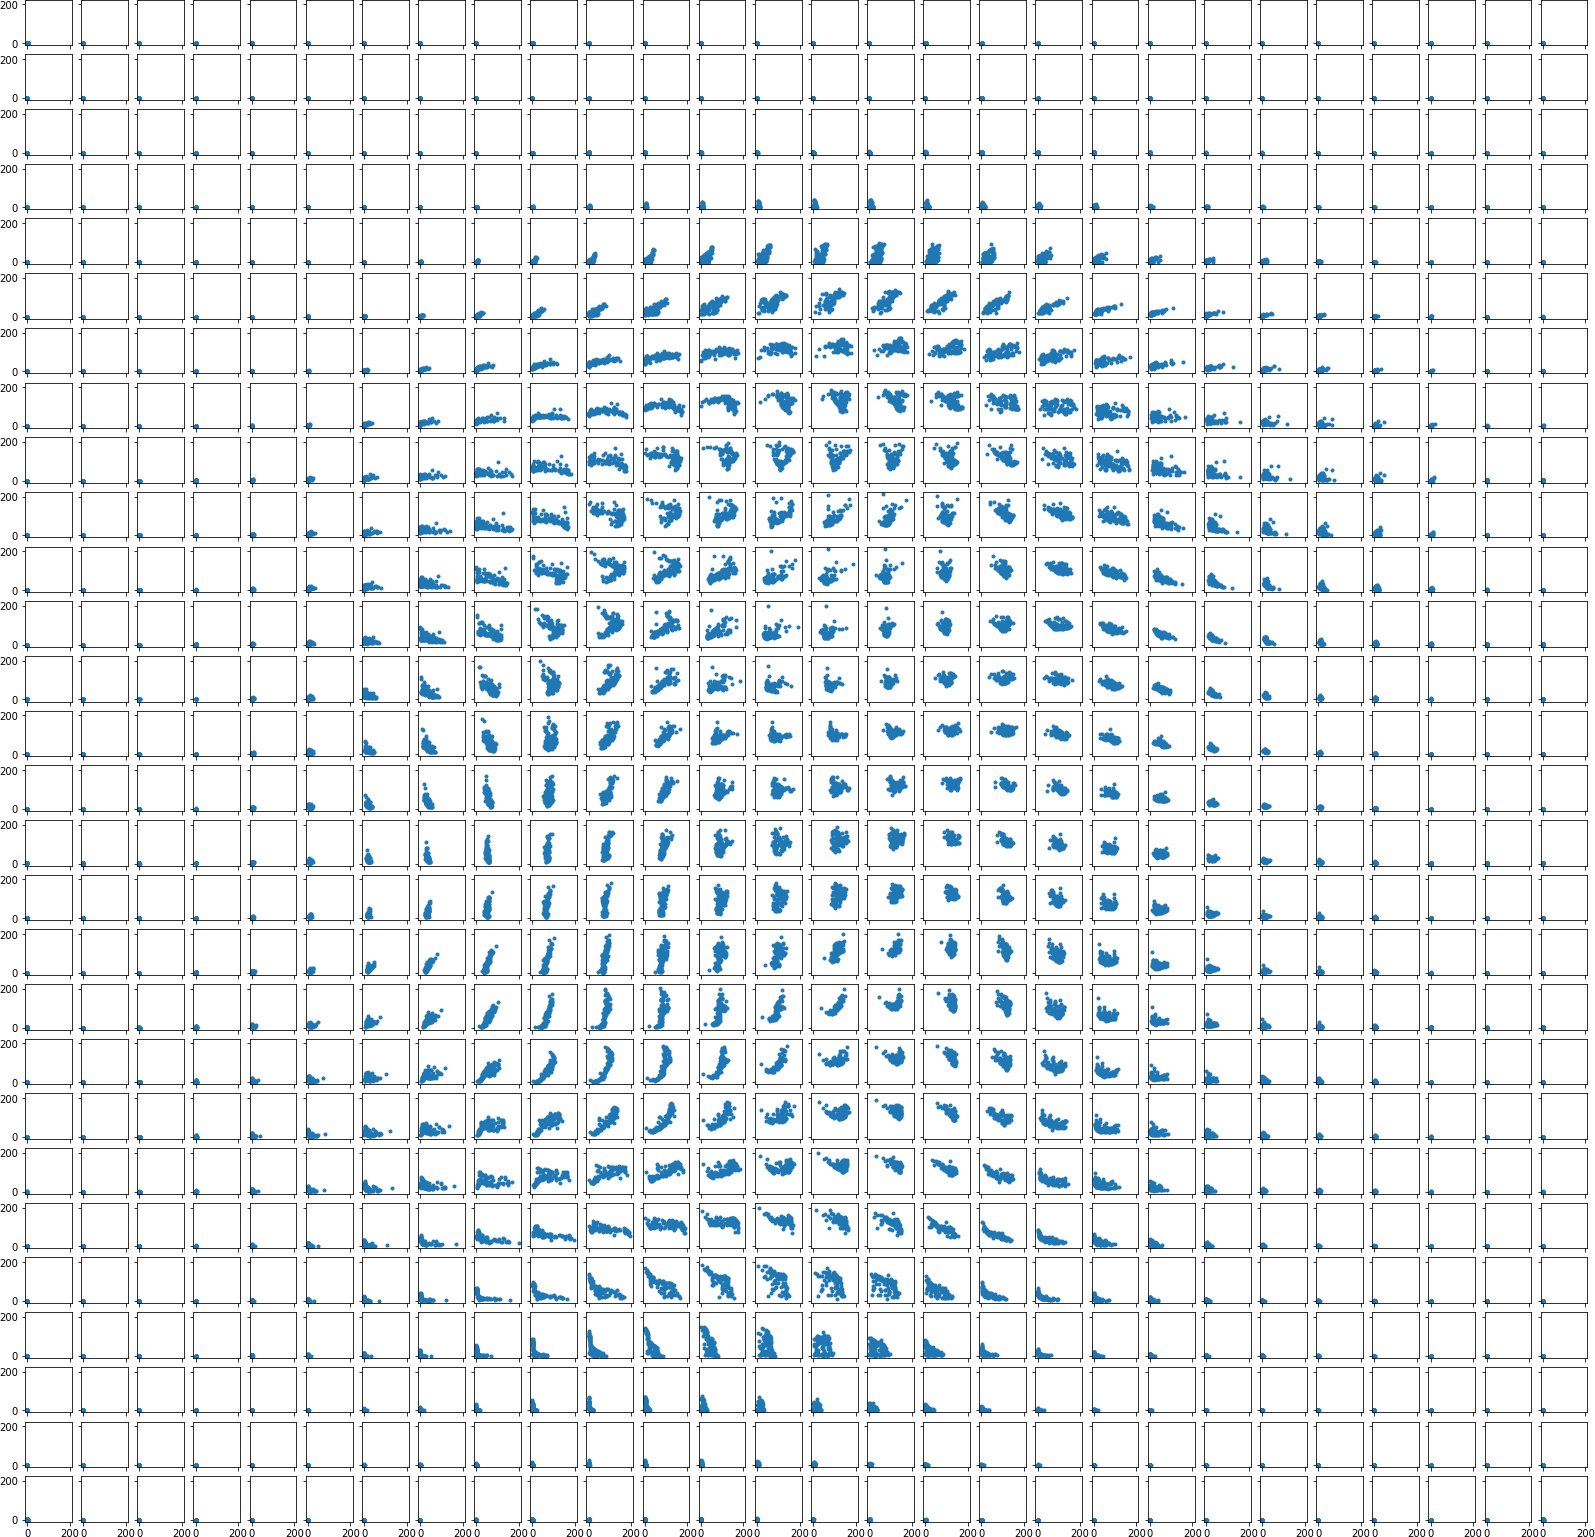
\includegraphics[width=\textwidth]{images/notprop.png}
    \caption{Proportionality of pixel intensities when fixing $\bm{z}_1 = \bm{z}_2=\varphi$. Each box represents one of $28\times 28$ MNIST pixels. The $x$-axis of each box encodes the mean pixel intensity of the $\bm{z}_1$-representative sample. The $y$-axis encodes the mean pixel intensity of the of the $\bm{z}_2$-representative sample. Dots within boxes belong to the same $\varphi$ for both, $\bm{z}_1$ and $\bm{z}_2$. }
    \label{fig:notprop}
\end{figure}

However, this is not true.
Choosing a value $\bm{z}_1 = \varphi$ such that $p_\theta(\bm{x} | \bm{z}_1 = \varphi)$ also leads to a high value of $p_\theta(\bm{x} | \bm{z}_2 = \varphi)$, leading to a violation of Equation \ref{eq:notprop}.

Consider Figure~\ref{fig:notprop}.
It shows results of samples $(\bm{x}_1^1,\bm{x}_2^1),\dots,(\bm{x}_1^{100},\bm{x}_{100}00)$ that were generated by Algorithm~\ref{alg:layer_representative_samples}\footnote{The results for the other combinations, $(\bm{z}_1,\bm{z}_3)$ and $(\bm{z}_2,\bm{z}_3)$ can be found in Appendix \ref{sec:additional-plots-for-section_independence}}.
Thus, the parameter \say{numSamples} is chosen as 100 and the parameter \say{numApproximations} is chosen as 300.
Each $\bm{x}_i^j$ is one generated MNIST image of size $28\times 28$ pixels.
Each box in Figure~\ref{fig:notprop} corresponds to one of these pixels, the box index corresponds to the pixel in the MNIST image.
The $x$-values of dots in the same box then correspond to $\bm{x}_1^1\big|_{(3,1)}, \dots, \bm{x}_1^{100}\big|_{(3,1)}$, i.e. the pixel intensities of one specific pixel (here: third row, first column (3,1)) over all 100 samples for $\bm{x}_1$, i.e. the sample generated by fixing $\bm{z}_1$.
Analogously, the $y$-values of dots in the same box correspond to $\bm{x}_2^1\big|_{(3,1)}, \dots, \bm{x}_2^{100}\big|_{(3,1)}$.
Each dot corresponds to one fixed $\varphi$-value.

Now, if changing the value of $\bm{z}_1$ was independent of changing the value of $\bm{z}_2$, the boxes should show now trend.
This is true for outer boxes.
They correspond to pixel values that always close to zero, therefore the value are in the bottom left corner and no correlation can be observed.
For center pixels, however, the plot shows something different.
They show an interesting correlation pattern of negative and positive correlations.

Negative correlations for a pixel with index $(i,j)$ indicate that $p_\theta(\bm{x}\big|_{(i,j)} | \bm{z}_1 = \varphi) \propto \frac{1}{p_\theta(\bm{x}\big|_{(i,j)} | \bm{z}_1 = \varphi)}$, i.e. choosing a value $\varphi$ that leads to a high $(i,j)$-pixel intensity for the $\bm{z}_1$-representative sample leads to a low intensity of the same pixel of the corresponding $\bm{z}_1$-representative sample.
This, however, is a violation of equation~\ref{eq:notprop}.
Importantly, the correlation only persists for certain pixels.

\textbf{Investigate, if possible, this in terms of Perceptual Path Length and Linear Separability (see \citet{karras2019style}).}

\subsection{Morpho-MNIST on VLAE}\label{subsec:morpho-mnist-on-vlae}

As discussed in Section~\ref{subsubsec:representation_learning}, the \acl{VLAE} aims at learning \say{hierarchical disentangled representation}~\citep{zhao2017learning}.
The lower embedding layers of such a model trained on MNIST (see Section~\ref{subsubsec:mnist}) encode features such as stroke width, digit width, and digit tilt whereas the highest layer mainly learns digit identity~\citep{zhao2017learning}.

\begin{figure}
    \centering
    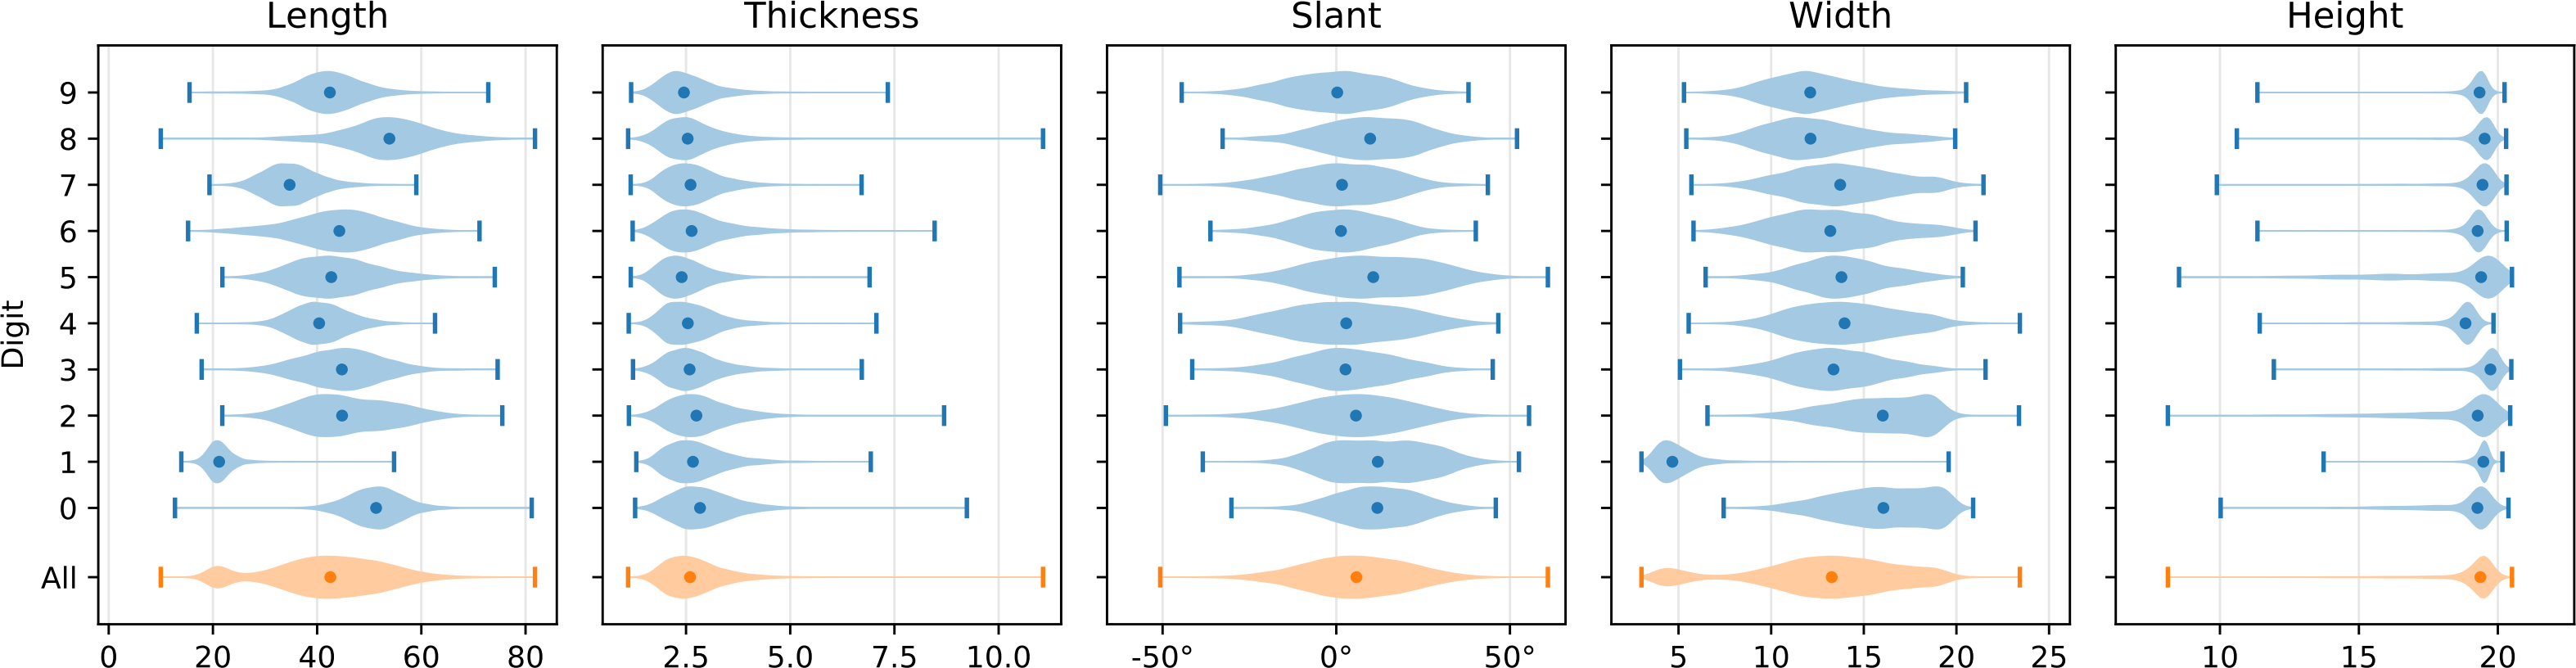
\includegraphics[width=\textwidth]{images/morpho_mnist_distribution.png}
    \caption{Distribution of the \textsc{Morpho-MNIST} attributes for the different digits. Taken from \citep{castro2019morpho}.}
    \label{fig:morpho_mnist_distribution}
\end{figure}

Incorporating the additional labels provided by Morpho-\textsc{MNIST} (see Section~\ref{subsubsec:morphomnist}) helps to analyze to what extent the lower layers learn which morphological features of \textsc{MNIST}.
The morphological attributes, however, are not equally distributed for all digits.
The mean stroke length and the digith width, for example, have a very low mean value for the digit \say{1} (see Figure~\ref{fig:morpho_mnist_distribution}).
Therefore, it should be possible to almost uniquely identify the identity of the digit \say{1} by just considering the stroke length or the digit width.
Other attributes such as stroke thickness, digit slant, and digit height are more evenly distributed (see Figure~\ref{fig:morpho_mnist_distribution}).

\begin{figure}
    \centering
    \begin{subfigure}{.33\textwidth}
        \centering
        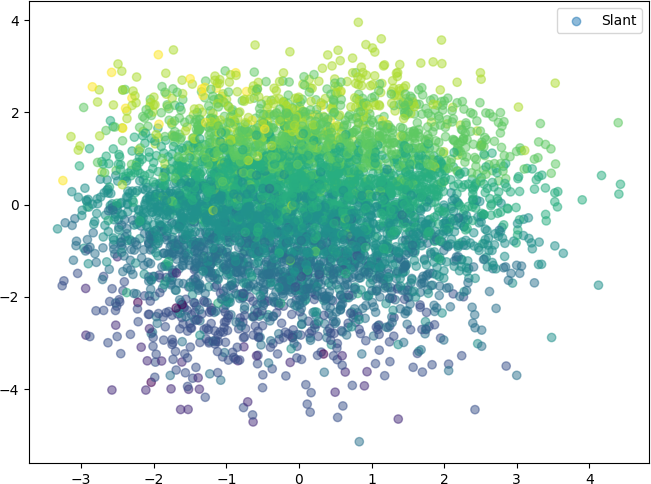
\includegraphics[width=\textwidth]{images/vlae_embeddings/embeddings_mu_1_0.png}
        \caption{}
        \label{fig:vlae_embeddings_mu1_slant}
    \end{subfigure}%
    \begin{subfigure}{.33\textwidth}
        \centering
        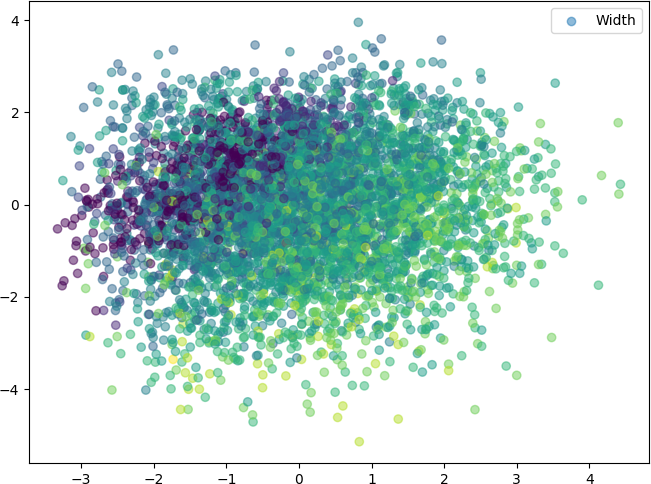
\includegraphics[width=\textwidth]{images/vlae_embeddings/embeddings_mu_1_4.png}
        \caption{}
        \label{fig:vlae_embeddings_mu1_width}
    \end{subfigure}
    \begin{subfigure}{.33\textwidth}
        \centering
        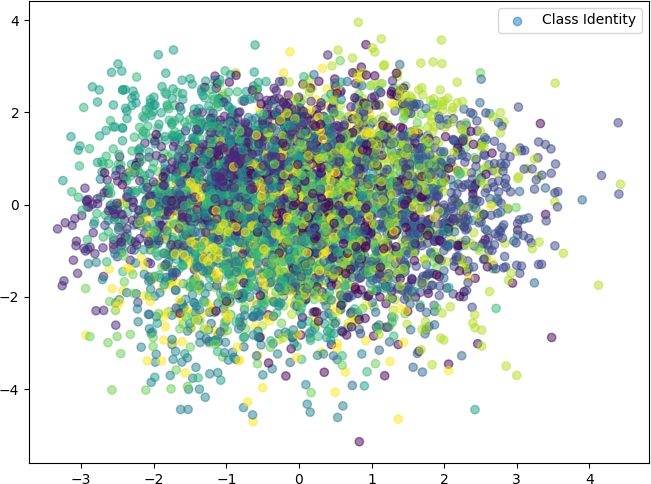
\includegraphics[width=\textwidth]{images/vlae_embeddings/embeddings_mu_1_6.png}
        \caption{}
        \label{fig:vlae_embeddings_mu1_identity}
    \end{subfigure}
    \caption{5000 random training points plotted in the first embedding layer $\bm{z}_1$ for the VLAE model. The position of the dots does not change in the diffent subplot. Different color dots by different means (shown in the respective legend). The morphological attributes are evenly assigned to ten bins. Dark colors indicate a low value of the respective whereas bright colors indicate a high value.}
    \label{fig:vlae_embeddings_mu1}
\end{figure}

Consider Figure~\ref{fig:vlae_embeddings_mu1_slant} showing the embedding layer $\bm{z}_1$ colored by digit slant\footnote{A complete plot of all morphological attributes for all layers can be found in Appendix~\ref{sec:additional-plots-for-section_morpho_mnist}.}.
Figure~\ref{fig:morpho_mnist_distribution} shows that the mean of the attribute \textit{Slant} is quite evenly distributed.
The color gradient in Figure~\ref{fig:vlae_embeddings_mu1_slant} therefore indicates that the VLAE actually learns the morphological attribute instead of just showing the class identity, encoded by means of another morphological attribute that correlates with class identity.

For Figure~\ref{fig:vlae_embeddings_mu1_width}, the situation is different.
The noticeable dark-purple cluster in the top left correlates with dark-purple points in Figure~\ref{fig:vlae_embeddings_mu1_identity} that encode image with label \say{1}.
For digit width, however, \say{1} is an outlier (see Figure~\ref{fig:morpho_mnist_distribution}) and a small digit width therefore is a strong indicator for a digit identity of \say{1}.
Not considering the dark-purple points, $\bm{z}_1$ still shows a less prominent color gradient from the bottom right to the top left.
In contrast, digit identity does not seem to be encoded strongly by $\bm{z}_1$ (see Figure~\ref{fig:vlae_embeddings_mu1_identity}).

\textbf{continue}

\subsection{Sparse Activations}
\textbf{DRAFT!}
Present results on feature map activities: most inactive, only a few active.
\citet{yoshida2020natural} show that natural images are sparsely encoded in mice V1, however in contrast to our results, the overlap for different images is quite small.
Discuss the implications on the model suitability.

\subsection{Feature Map Stripes}\label{subsec:feature-map-stripes}

\begin{figure}
    \centering
    \begin{subfigure}{0.3\textwidth}
        \centering
        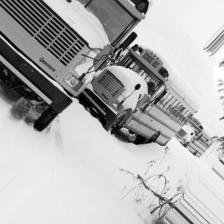
\includegraphics[width=\textwidth]{images/stripes/original.jpg}
        \caption{The original image.}
        \label{subfig:stripes_original}
    \end{subfigure}
    \hfill
    \begin{subfigure}{0.3\textwidth}
        \centering
        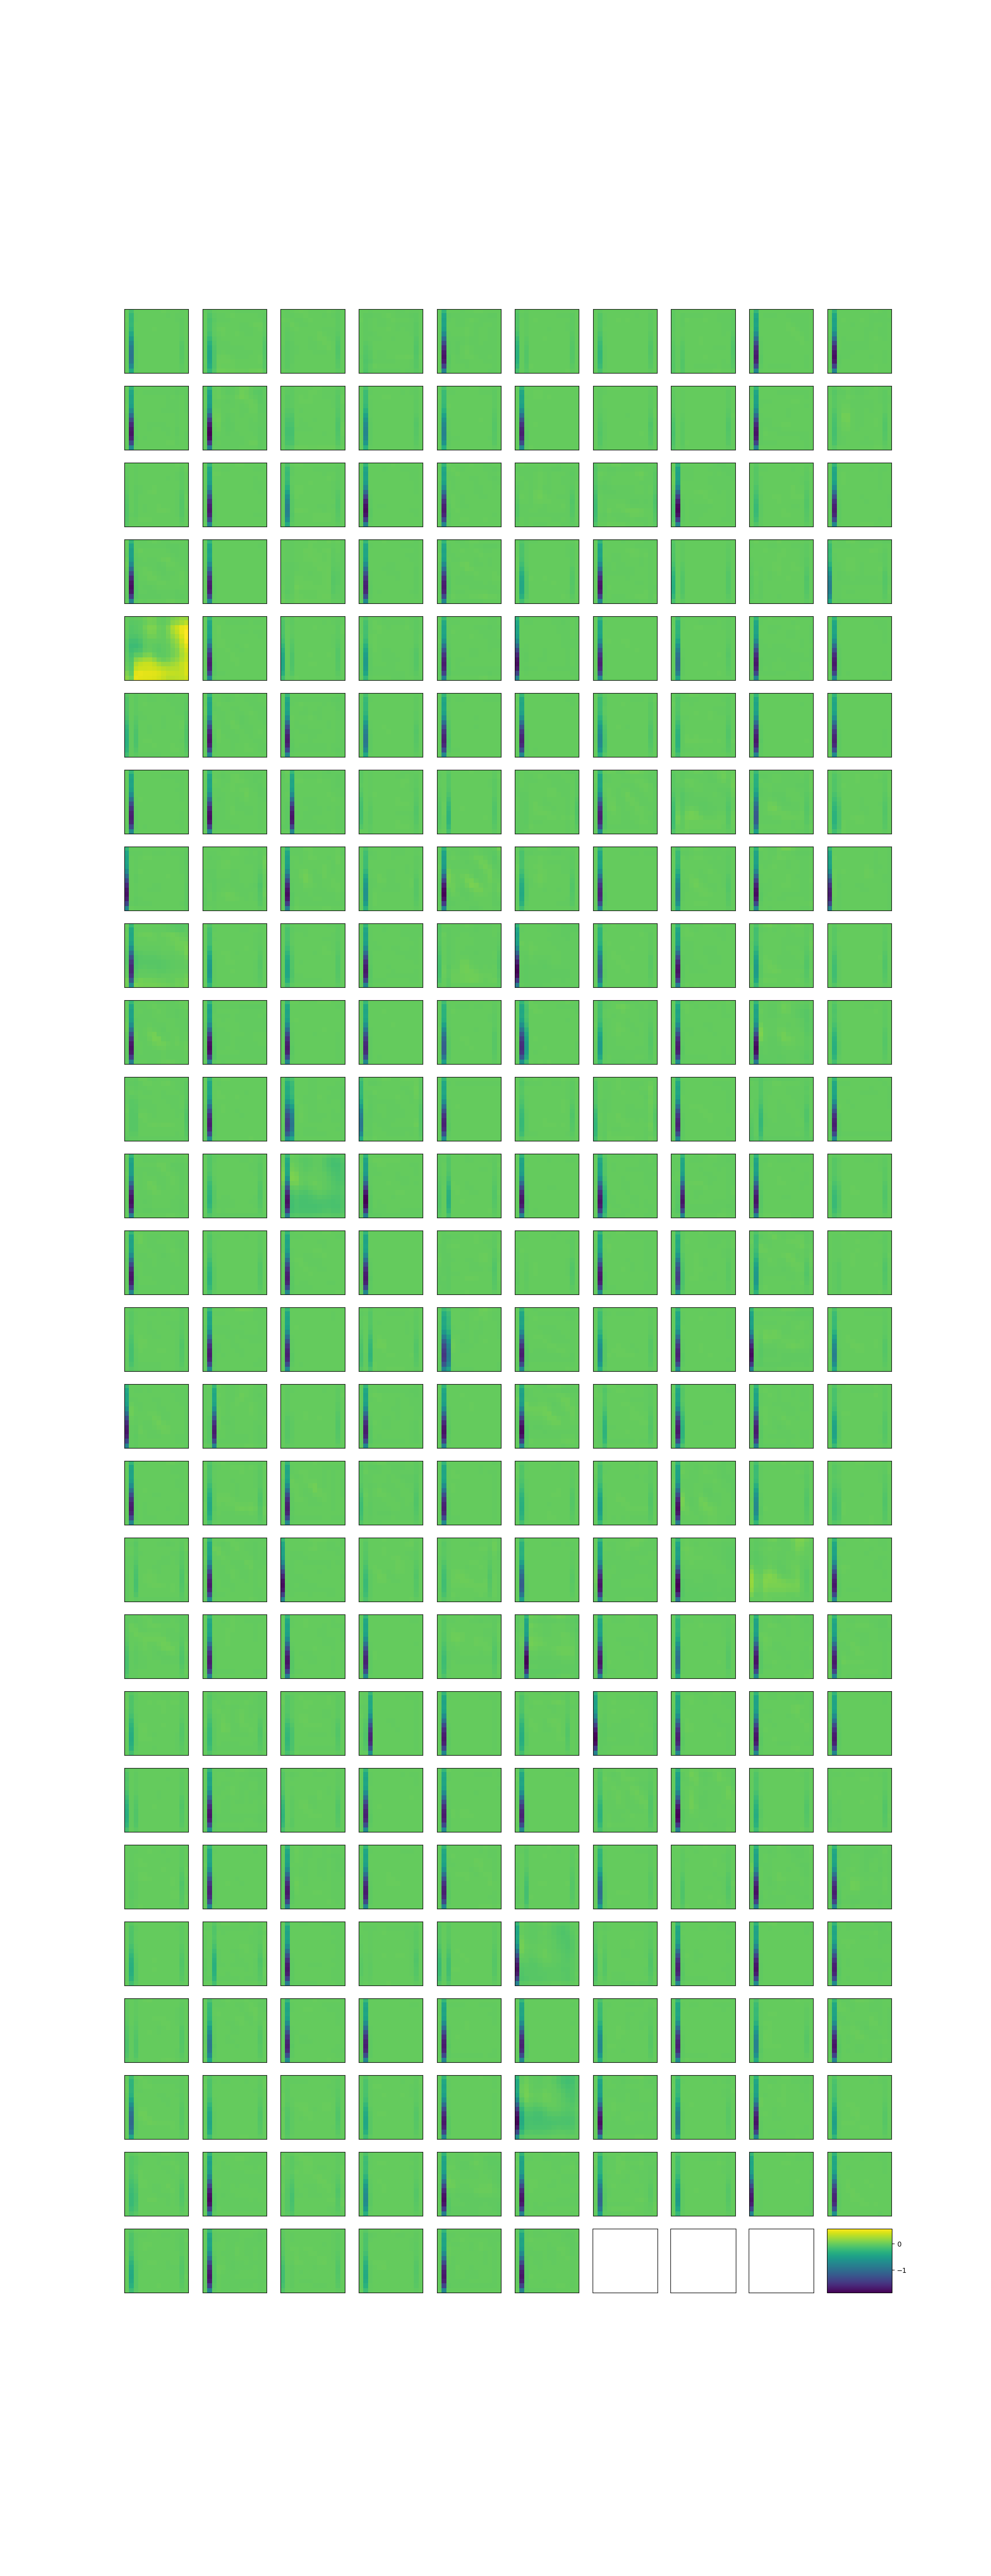
\includegraphics[width=\textwidth]{images/stripes/leaky_re_lu_5.png}
        \caption{The feature maps after LeakyReLU 5}
        \label{subfig:lakyrelu5}
    \end{subfigure}
    \hfill
    \begin{subfigure}{0.3\textwidth}
        \centering
        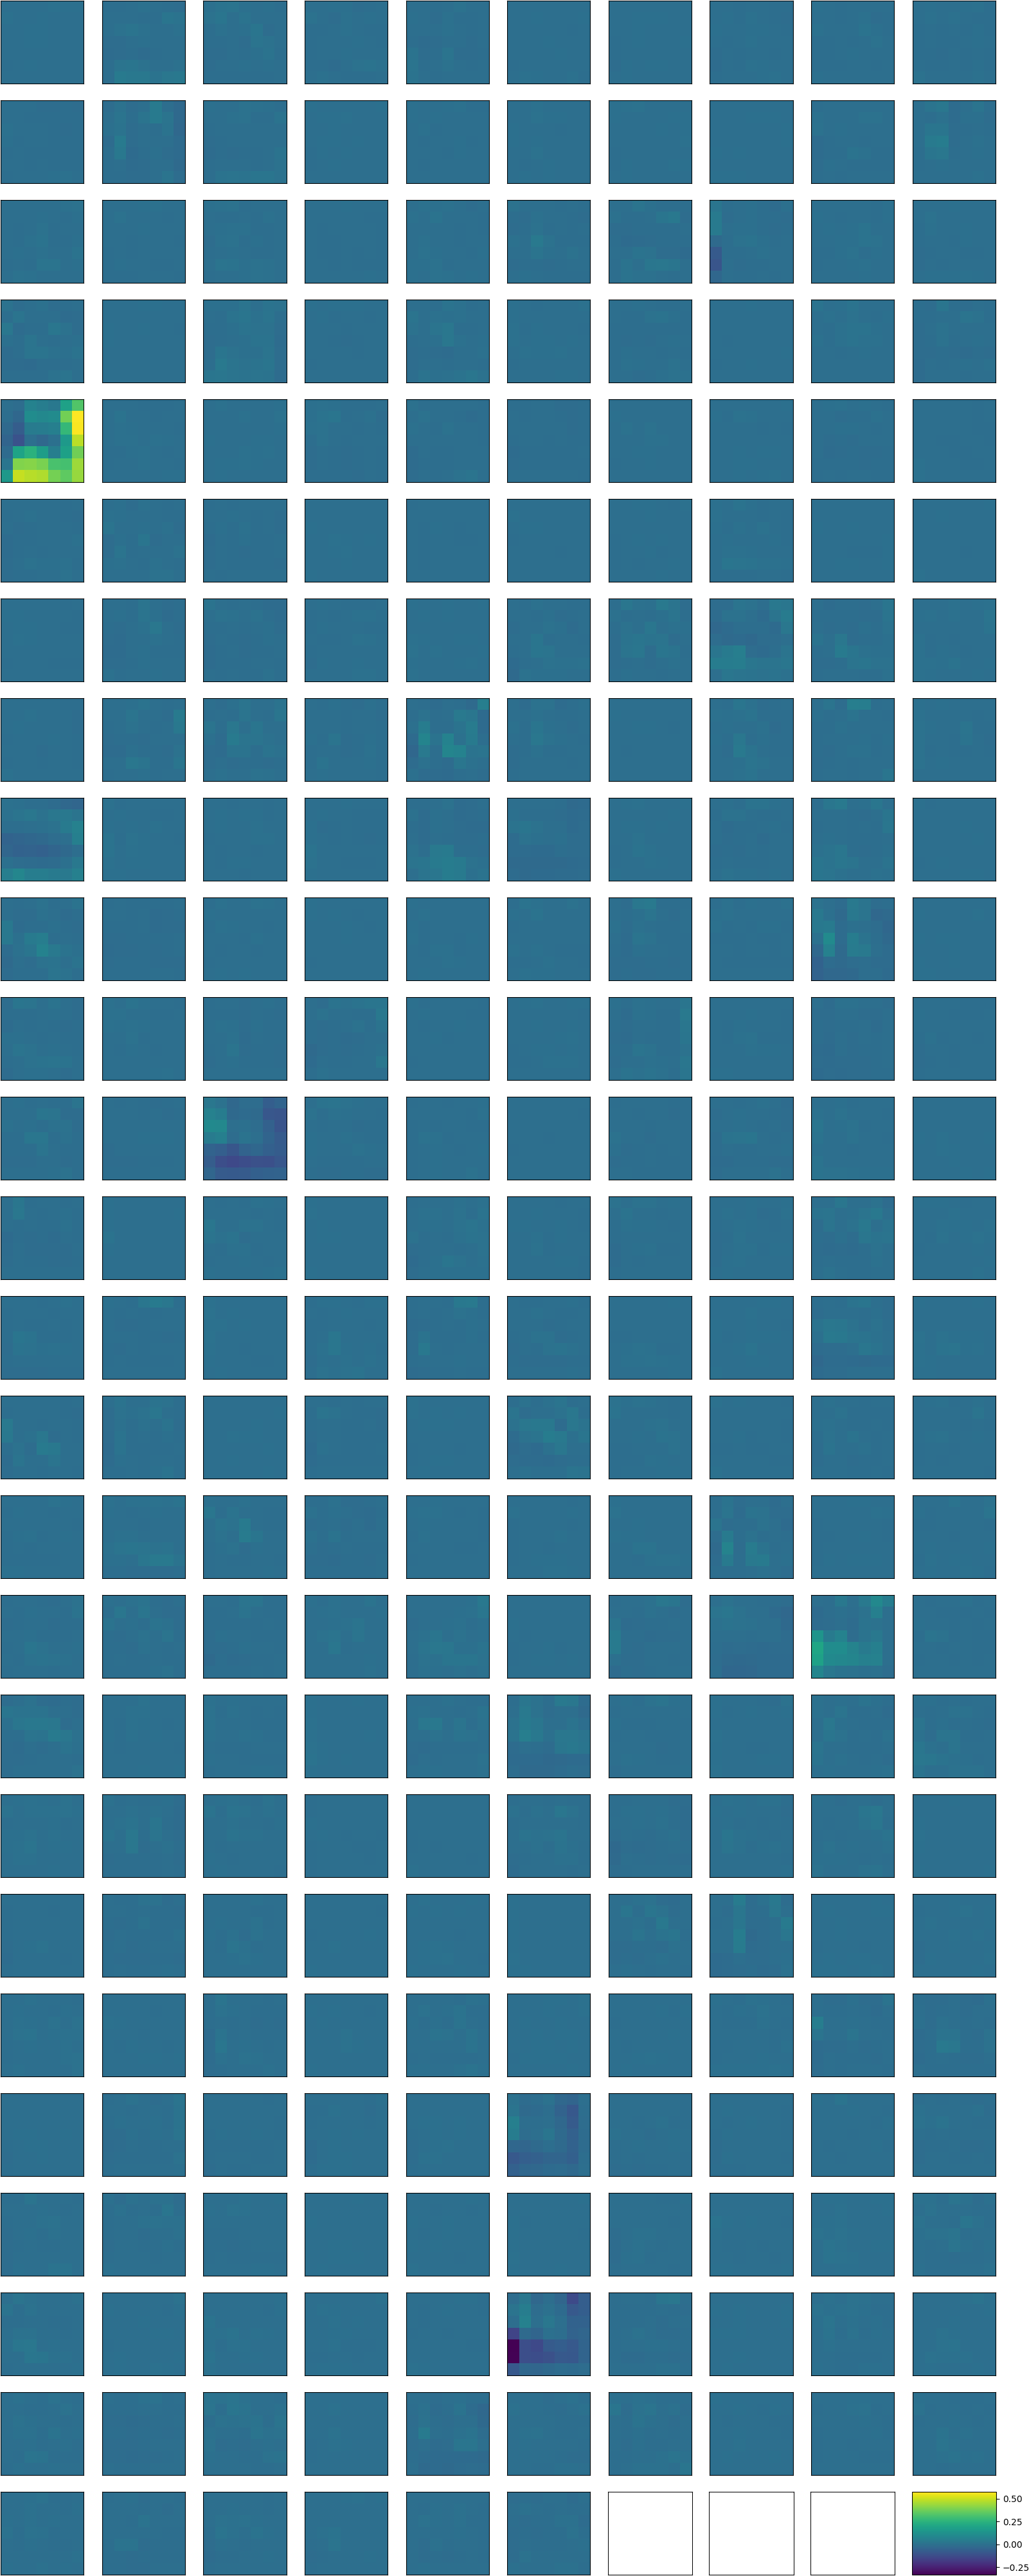
\includegraphics[width=\textwidth]{images/stripes/max_pooling2d_3.png}
        \caption{The feature maps after max pooling of LeakyReLU 5}
        \label{subfig:maxpool}
    \end{subfigure}
    \caption{The original image and the feature maps after passing the image through the network until after the specified layer. The stripe artifacts can be observed in many feature maps in Subfigure~\ref{subfig:lakyrelu5}. They vanish after max-pooling (Subfigure~\ref{subfig:maxpool}).}
    \label{fig:stripes}
\end{figure}


One observation being made during the analysis of the networks was the emergence of striped artifacts in the networks feature maps (Figure~\ref{fig:stripes}).
These stripes were observed in the Vanilla VAE, AlexNetVAE, as well as the AlexNet Classifier and might be also present in other networks (\textbf{CHECK THIS}).
Apparently, the stripes are either always horizontal or vertical for one network type.
If they are vertical, they can appear on the left or the right side of the same network.
If they are horizontal, they appear either on the top or on the bottom of the same network.
The exact reason why the networks show this behavior was not found, however some insights were won.

\paragraph{Padding}
The stripes occur due to the zero-padding in the network and the resulting contrast observed by the convolutional filters.
Take Figure~\ref{fig:stripes}.
Here, the stripes appear strongest on the bottom left of the image.
Noteworthy, the stripes indicate less active regions in the feature map: The feature map has an activity of around zero everywhere except for the location of the stripes.
Here, the activity is strongly negative.

A comparison with the original image (Figure~\ref{subfig:stripes_original}) shows that for the left side of the image, the contrast is highest on the bottom if the image is zero-padded\footnote{Zero-padding can be understood as adding black pixels around the image.}.
Importantly, the contrast is as high on the bottom of the image, the right side, and the right side of the top of the image.
However, for this network, the stripes seem to occur for a sharp shift of black on the left to white on the right.

\begin{figure}
    \centering
    \foreach \n in {0,...,11}{
        \begin{subfigure}{0.05\textwidth}
            \frame{\includegraphics[width=\textwidth]{images/stripes/test_images/original\n.jpg}}
            \caption{}
            \label{subfig:test_images_stripes\n}
        \end{subfigure}
        \hfill
    }
    \caption{The test images used to analyze the networks behavior.}
    \label{fig:test_images_stripes}
\end{figure}

To better understand the behavior, the network was applied to a set of artifical test images (Figure~\ref{fig:test_images_stripes}).
All different feature maps with respect to each image can be found in the appendix.

\begin{figure}
    \centering
    \begin{subfigure}{0.45\textwidth}
        \centering
        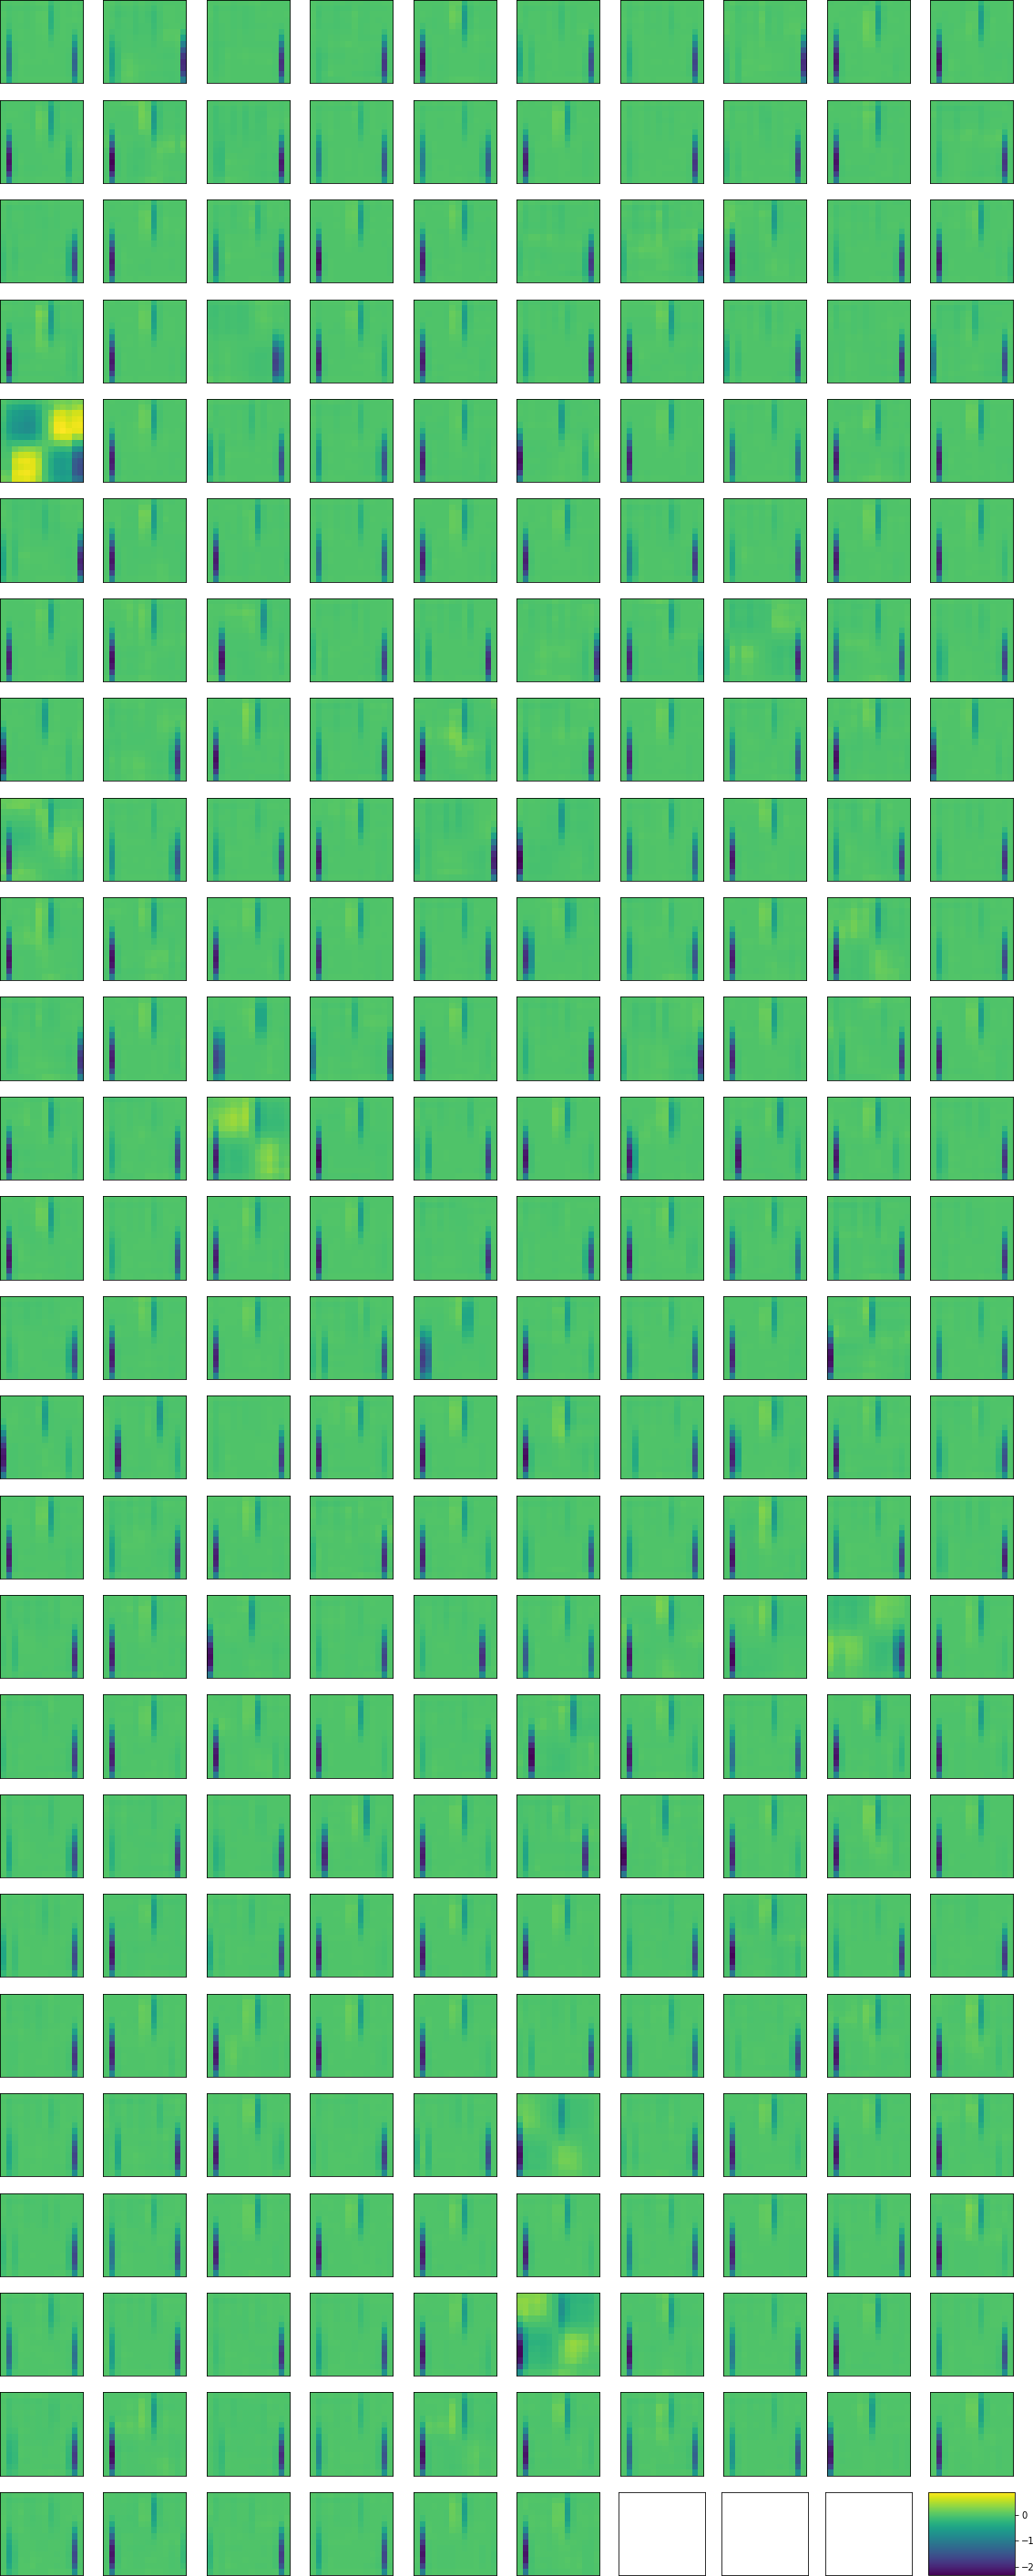
\includegraphics[width=\textwidth]{images/stripes/test_img_9/leaky_re_lu_5.png}
        \caption{The original image.}
        \label{subfig:stipes_test_img_leakyrelu5}
    \end{subfigure}
    \hfill
    \begin{subfigure}{0.45\textwidth}
        \centering
        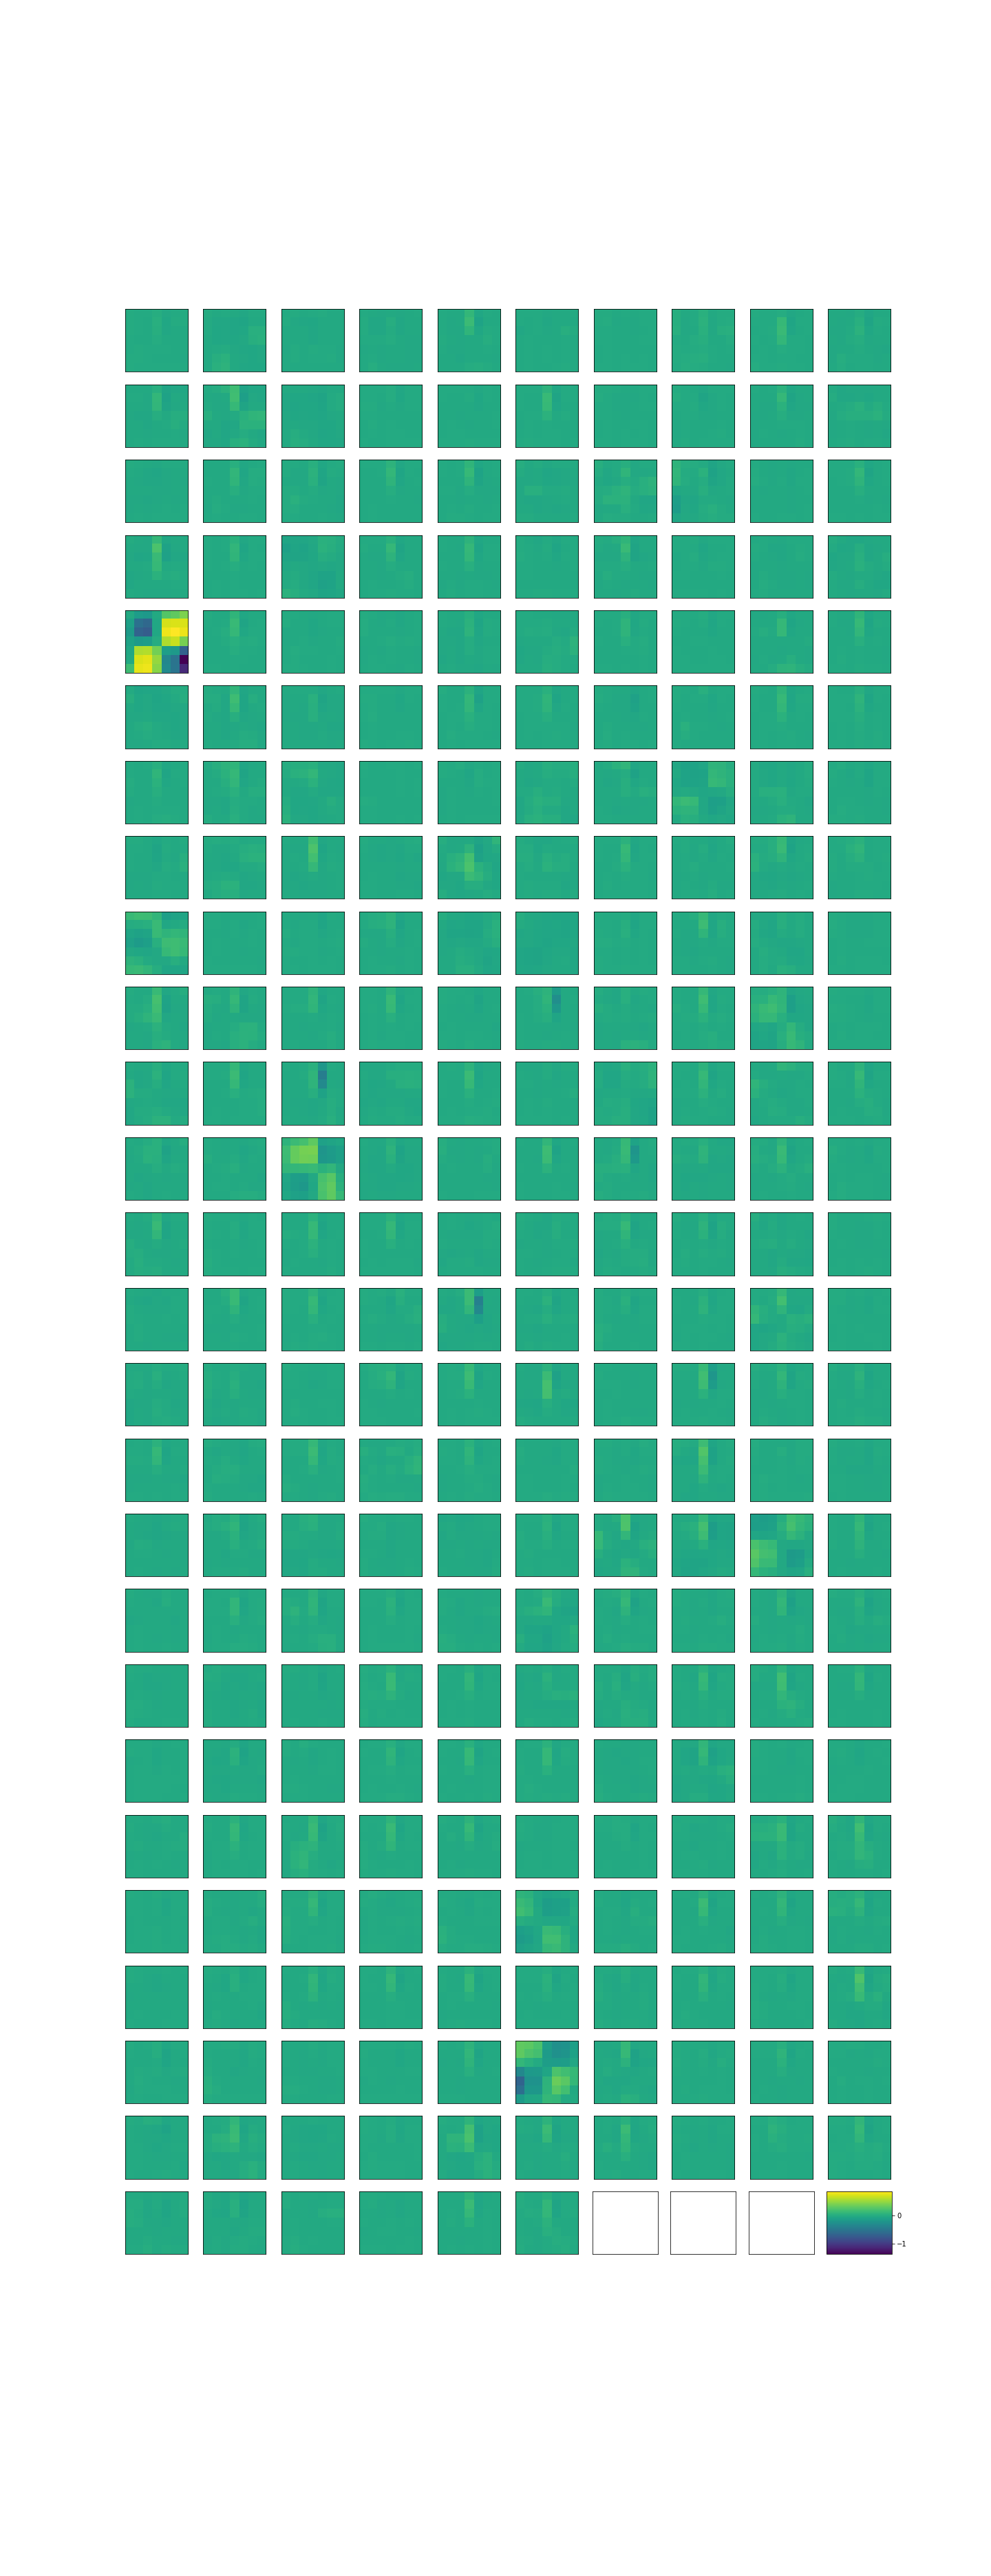
\includegraphics[width=\textwidth]{images/stripes/test_img_9/max_pooling2d_3.png}
        \caption{The feature maps after LeakyReLU 5}
        \label{subfig:stripes_test_img_maxpool3}
    \end{subfigure}
    \caption{The feature maps with respect to test image~\ref{subfig:test_images_stripes8}.}
    \label{fig:stripes_test_img}
\end{figure}

Subfigure~\ref{subfig:test_images_stripes8} and~\ref{subfig:test_images_stripes11} turned to be most equally high insightful.
Figure~\ref{fig:stripes_test_img} shows the feature map after the last LeakyReLU (LeakyReLU 5) activation of the network given this input image (Subfigure~\ref{subfig:stipes_test_img_leakyrelu5}) as well as the feature map after max-pooling of this feature map (Subfigure~\ref{subfig:stripes_test_img_maxpool3}).
Multiple things can be observed in Subfigure~\ref{subfig:stipes_test_img_leakyrelu5}.
Firstly, the feature map in the first column of the fifth row resembles the input stimulus itself.
The fact that this feature map shows most of the activity (especially after max-pooling, see Subfigure~\ref{subfig:stripes_test_img_maxpool3}) has been observed for natural images as well, however not the resemblance of the input stimulus.
Except for this feature map, stripes emerge either on the bottom of the left side or the bottom of the right side of the feature map.
For the bottom of the left side, this is where the sharp black-white contrast is.
The bottom of the right side is more complicated.
Here the test image was black and the \say{contrast} is a black-black contrast - or no contrast at all.
However, this is only true for the first feature map\footnote{The first feature maps are not shown here.}.
The following feature maps, again, are zero-padded.
However, due to the bias term in the convolutions, these might be non-zero in the bottom-right and top-left square of the image, thus leading to a contrast.
This explains why the network can be sensitive towards these black-black contrasts in the input image.

Noteworthy, if the bias term in the convolutions is removed, the black-black contrast sensitivity vanishes because the network is not able anymore to add a constant to the black pixel values on the bottom-right or top-left of the image.
For this purpose, the batch normalization has to be removed too since it uses a bias term as well.
This, however, does not qualitatively change the networks behavior on real images.



\section{Conclusion}\label{sec:conclusion}

This thesis discussed if \acfp{VAE} are candidate models of the visual cortex, potentially allowing to obtain semantic representations of the input.
Only little evidence has been found that \acp{VAE} and other related models have this property, suggesting that these models at least need to be modified to be good models of the visual system.
A more pessimistic conclusion is that unsupervised models per se are unfit models of the visual system.

This, however, leads to the question why supervised explain \ac{IT} activity better than unsupervised models.

One assumption is that the brain also mainly learns in a supervised manner and that supervision is always required to build realistic models of the brain.
This assumption seems to be too naive for a variety of reasons.

First, the models discussed in this thesis are too unrelated to the brain to allow such a conclusion.
The role of top-down connections as well as the role of sequential data has not been investigated thoroughly.
Furthermore, there are unsupervised models leading to Gabor wavelets~\citep{berkes2005slow}.
This is another hint that unsupervised models in general might be suitable models but need more refinement.

This thesis ruled out a family of models (\acp{VAE} and \acp{VLAE} in particular) as good models of the visual system.
But also, this thesis discussed ways to extend these models to better model the visual cortex and the emergence of semantic representations, suggesting multiple approaches for future research.

\newpage
\printbibliography

\newpage
\pagenumbering{Roman}
\setcounter{page}{\thesavepage}
\appendix
\section{Additional Plots for Section~\ref{subsec:independence-of-vlae-embeddings}}\label{sec:additional-plots-for-section_independence}
\begin{figure}[H]
\centering
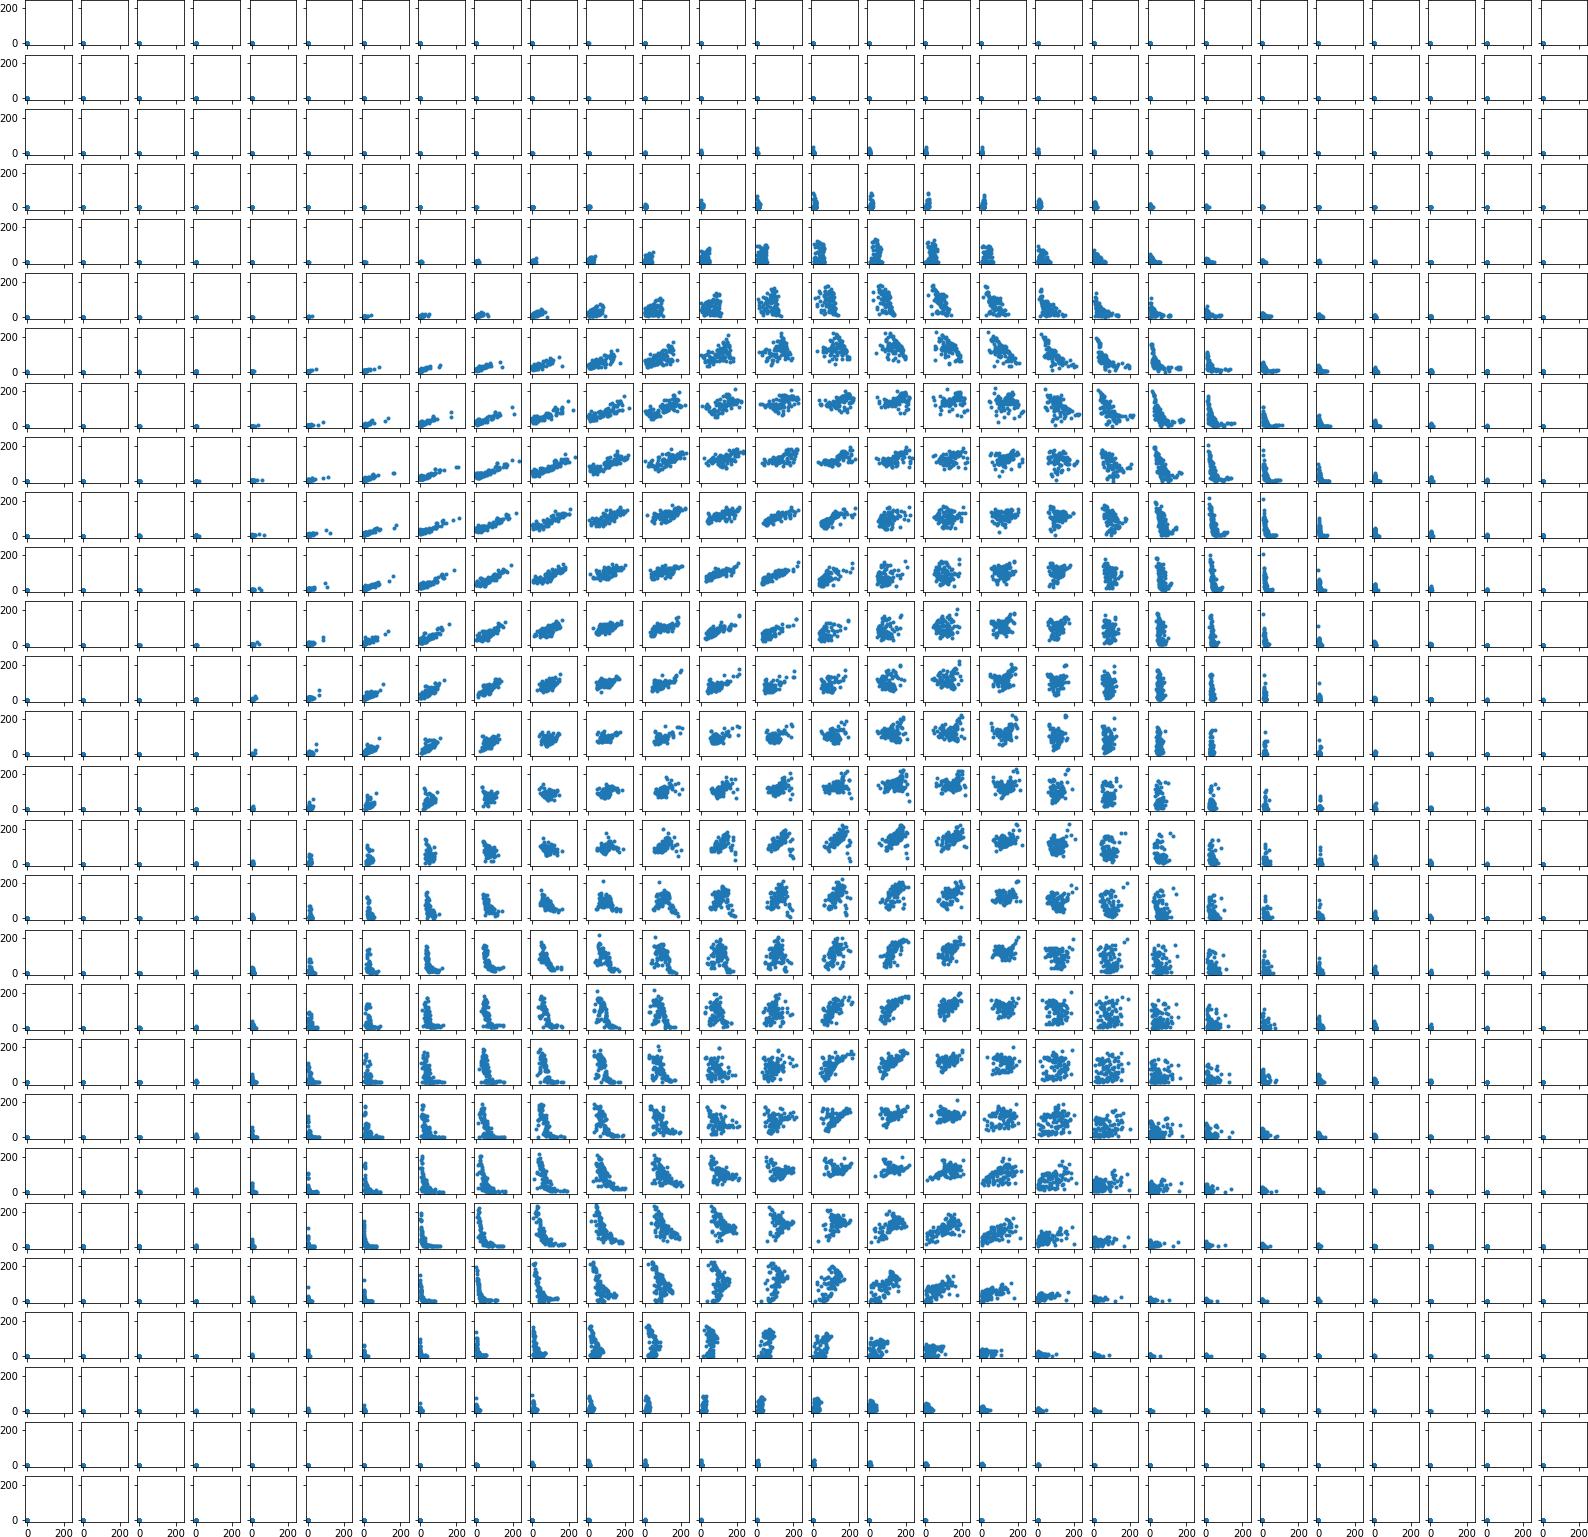
\includegraphics[width=\textwidth]{images/notprop/mnist/vlae/ccs_0_2_vlae.png}
\caption{Proportionality of pixel intensities when fixing $\bm{z}_1 = \bm{z}_3=\varphi$ for \ac{VLAE} on \textsc{Mnist}. Created accordingly to Figure~\ref{fig:notprop}.}
\end{figure}

\begin{figure}[H]
\centering
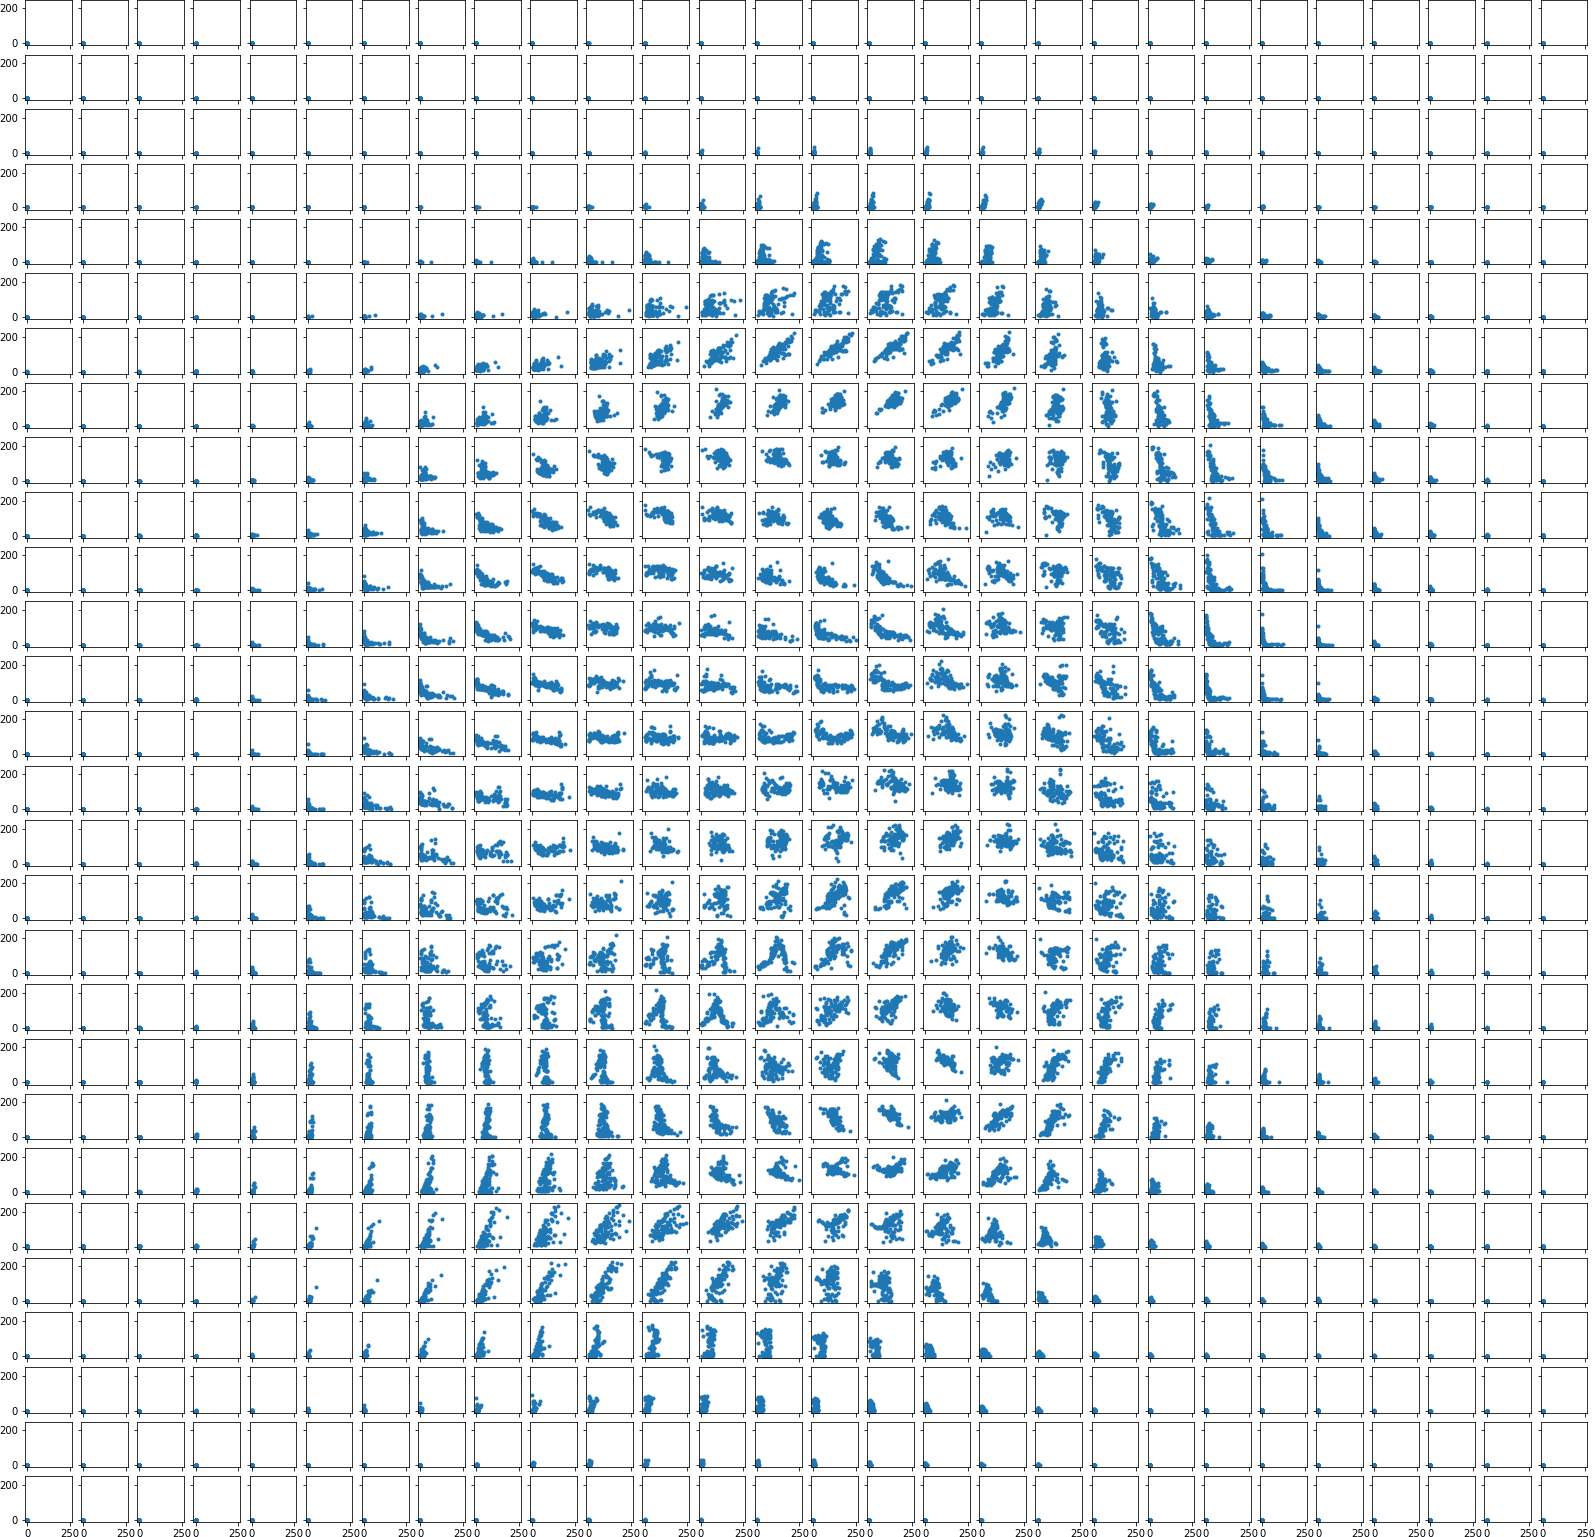
\includegraphics[width=\textwidth]{images/notprop/mnist/vlae/ccs_1_2_vlae.png}
\caption{Proportionality of pixel intensities when fixing $\bm{z}_2 = \bm{z}_3=\varphi$ for \ac{VLAE} on \textsc{Mnist}. Created accordingly to Figure~\ref{fig:notprop}.}
\end{figure}

\begin{figure}[H]
\centering
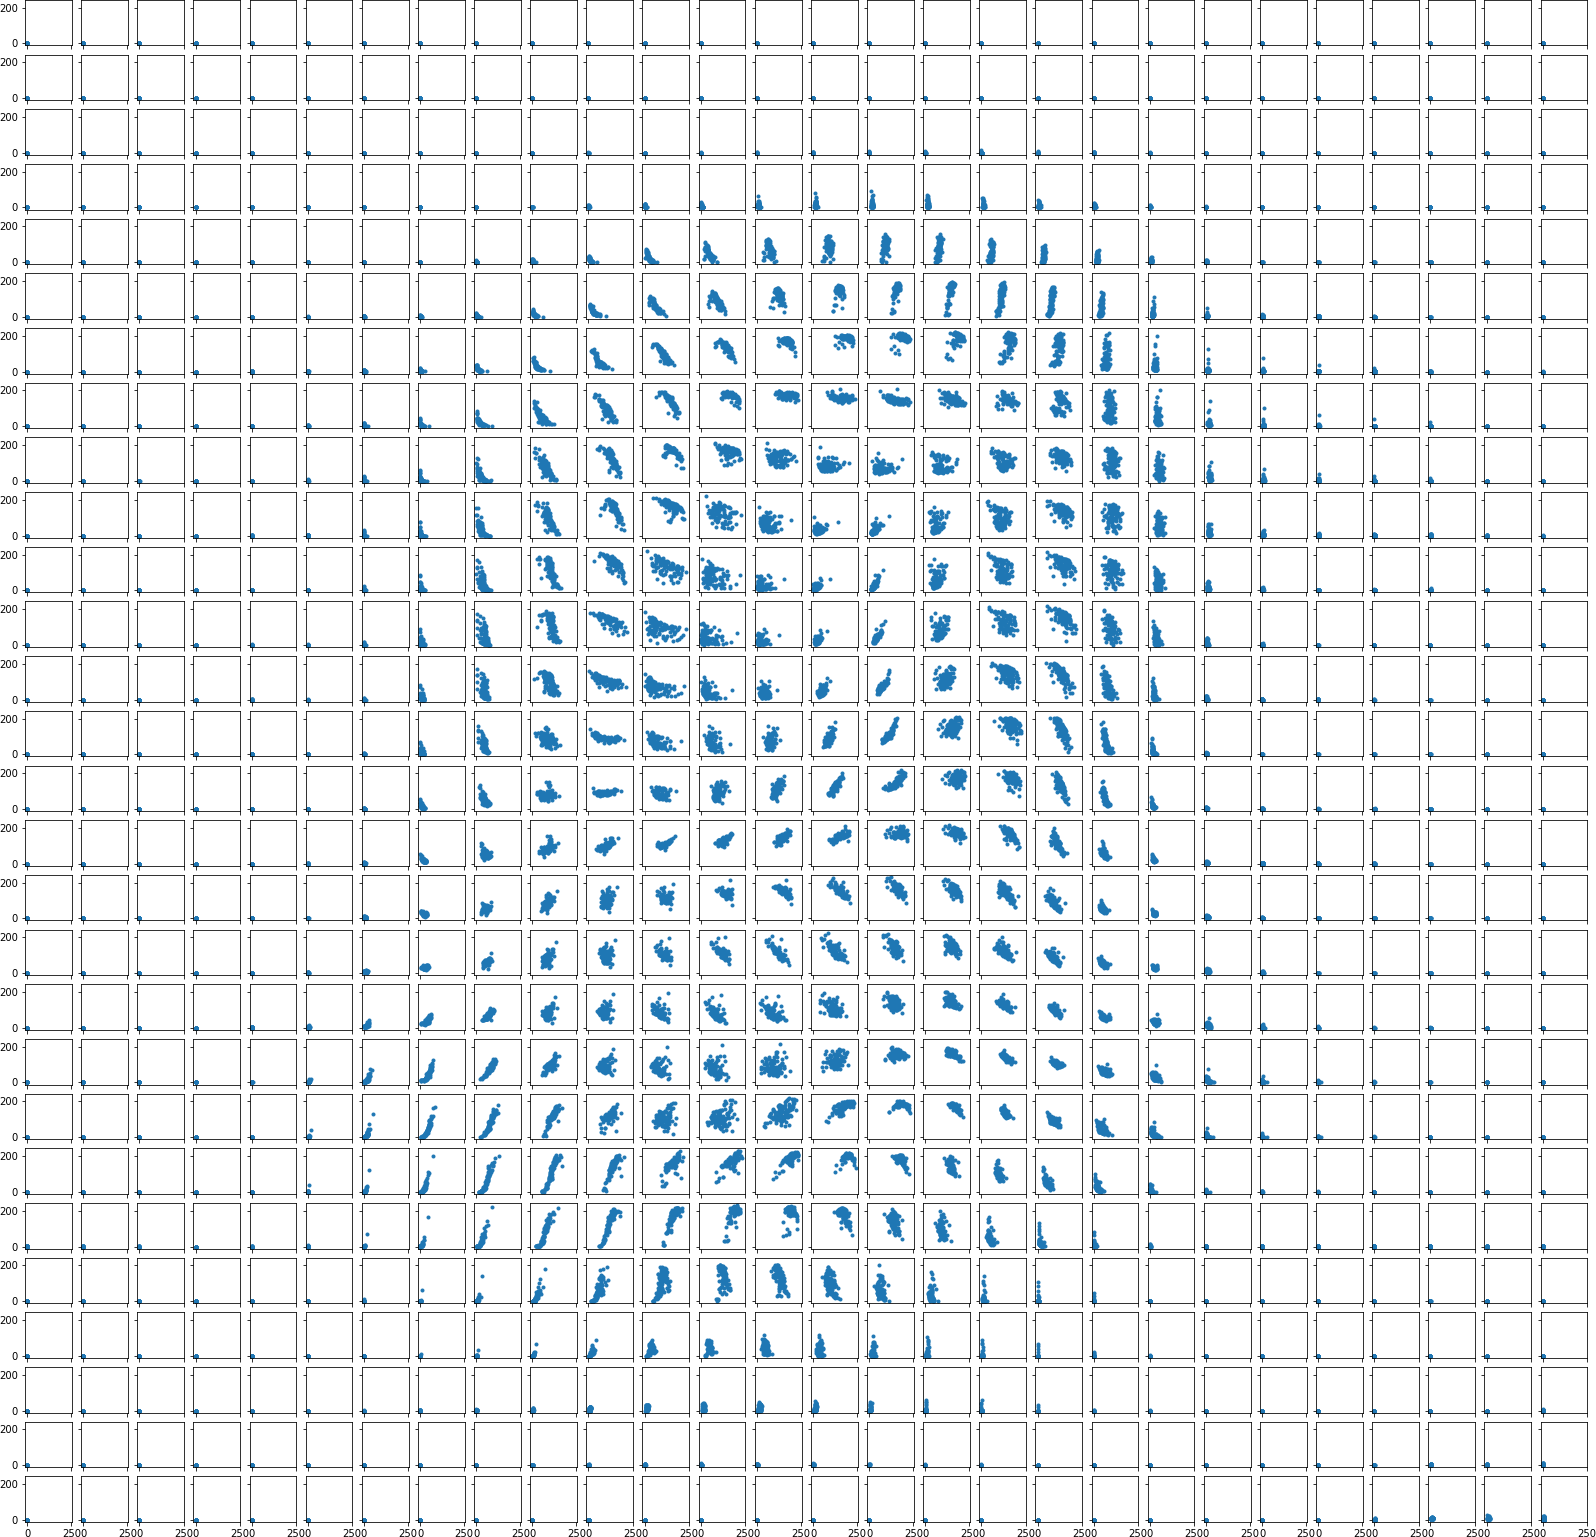
\includegraphics[width=\textwidth]{images/notprop/mnist/vlae_gan/ccs_0_1_vlae_gan.png}
\caption{Proportionality of pixel intensities when fixing $\bm{z}_1 = \bm{z}_2=\varphi$ for \ac{VLAE}-\ac{GAN} on \textsc{Mnist}. Created accordingly to Figure~\ref{fig:notprop}.}
\end{figure}

\begin{figure}[H]
\centering
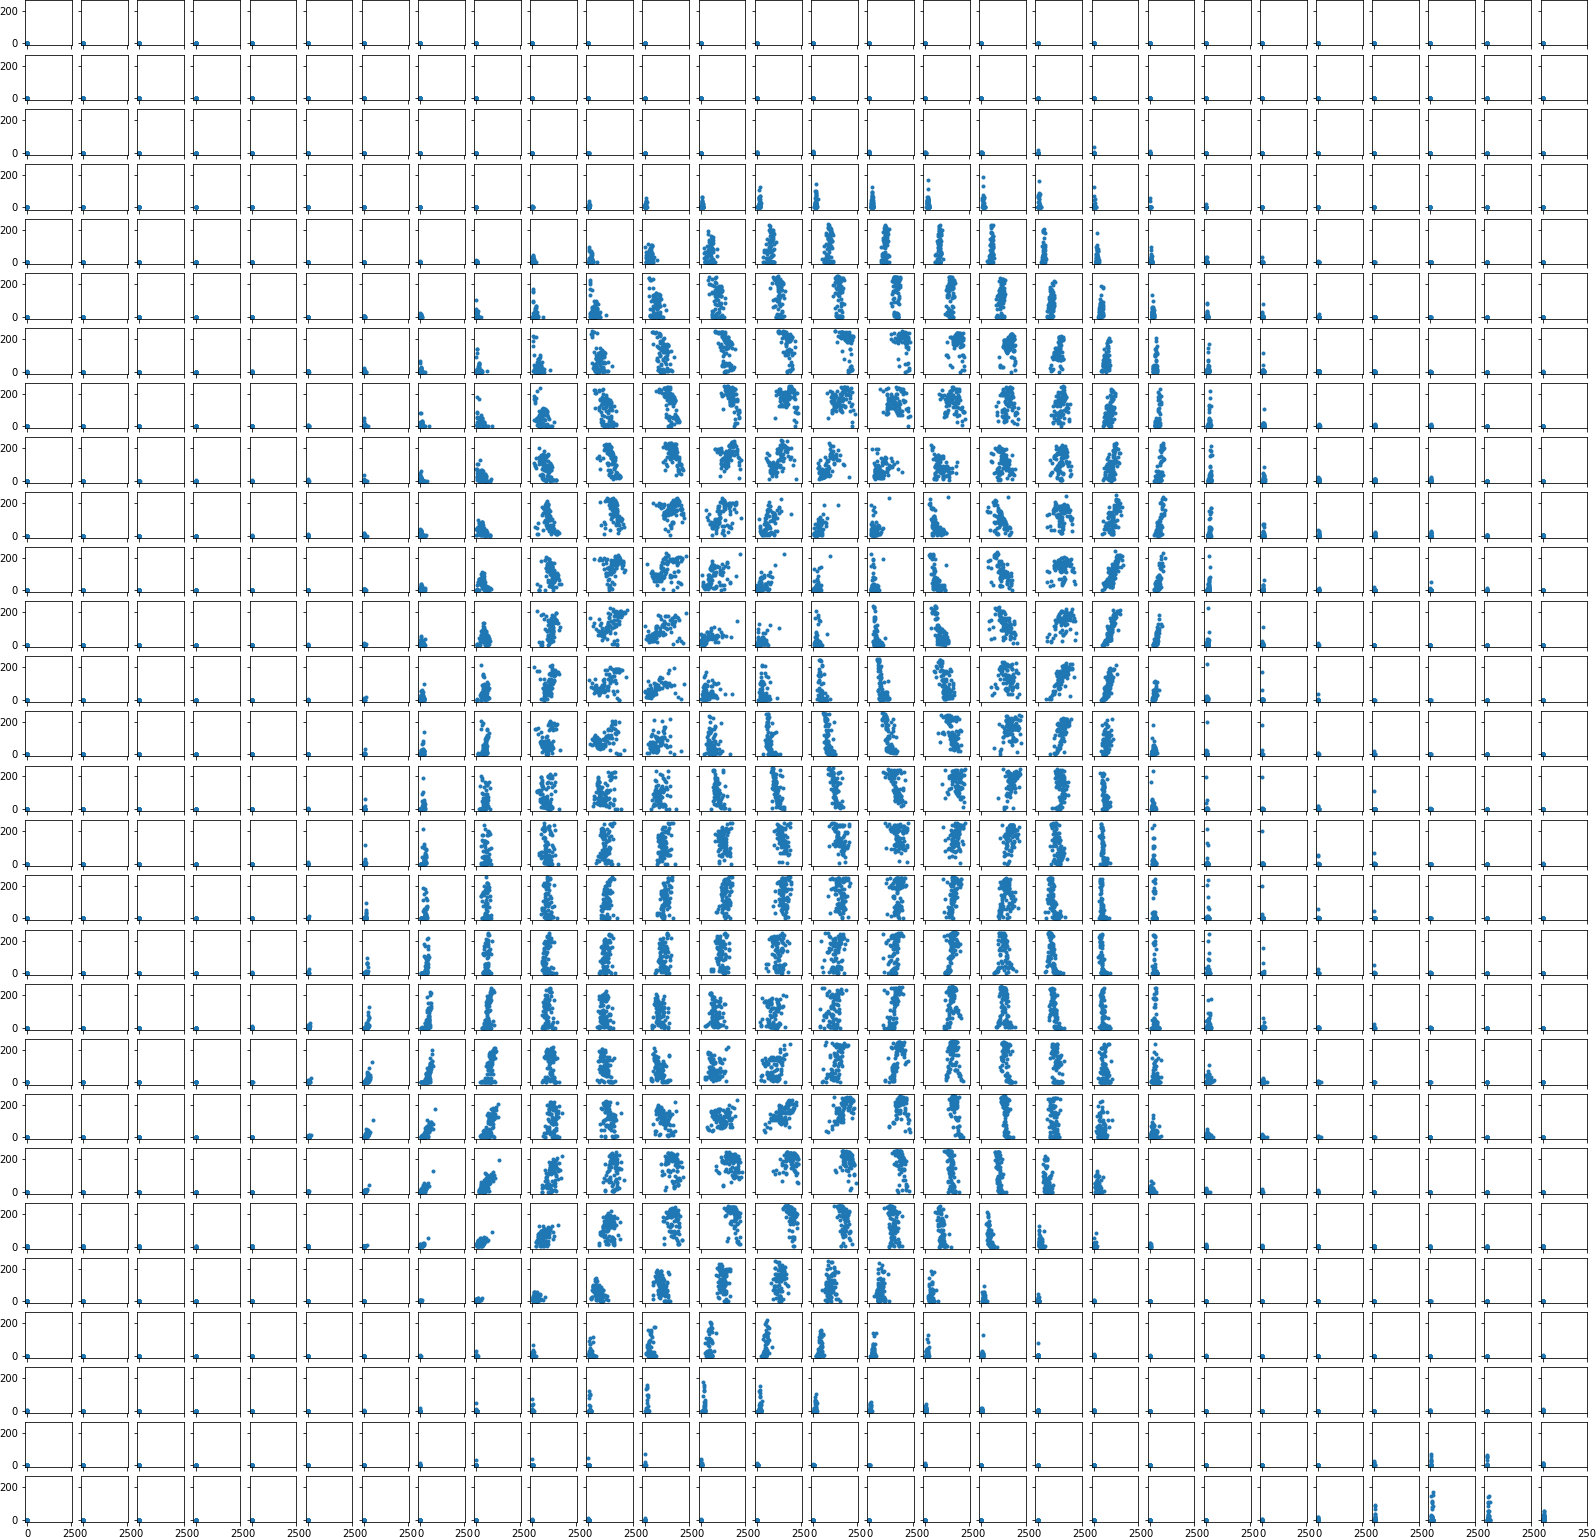
\includegraphics[width=\textwidth]{images/notprop/mnist/vlae_gan/ccs_0_2_vlae_gan.png}
\caption{Proportionality of pixel intensities when fixing $\bm{z}_1 = \bm{z}_3=\varphi$ for \ac{VLAE}-\ac{GAN} on \textsc{Mnist}. Created accordingly to Figure~\ref{fig:notprop}.}
\end{figure}

\begin{figure}[H]
\centering
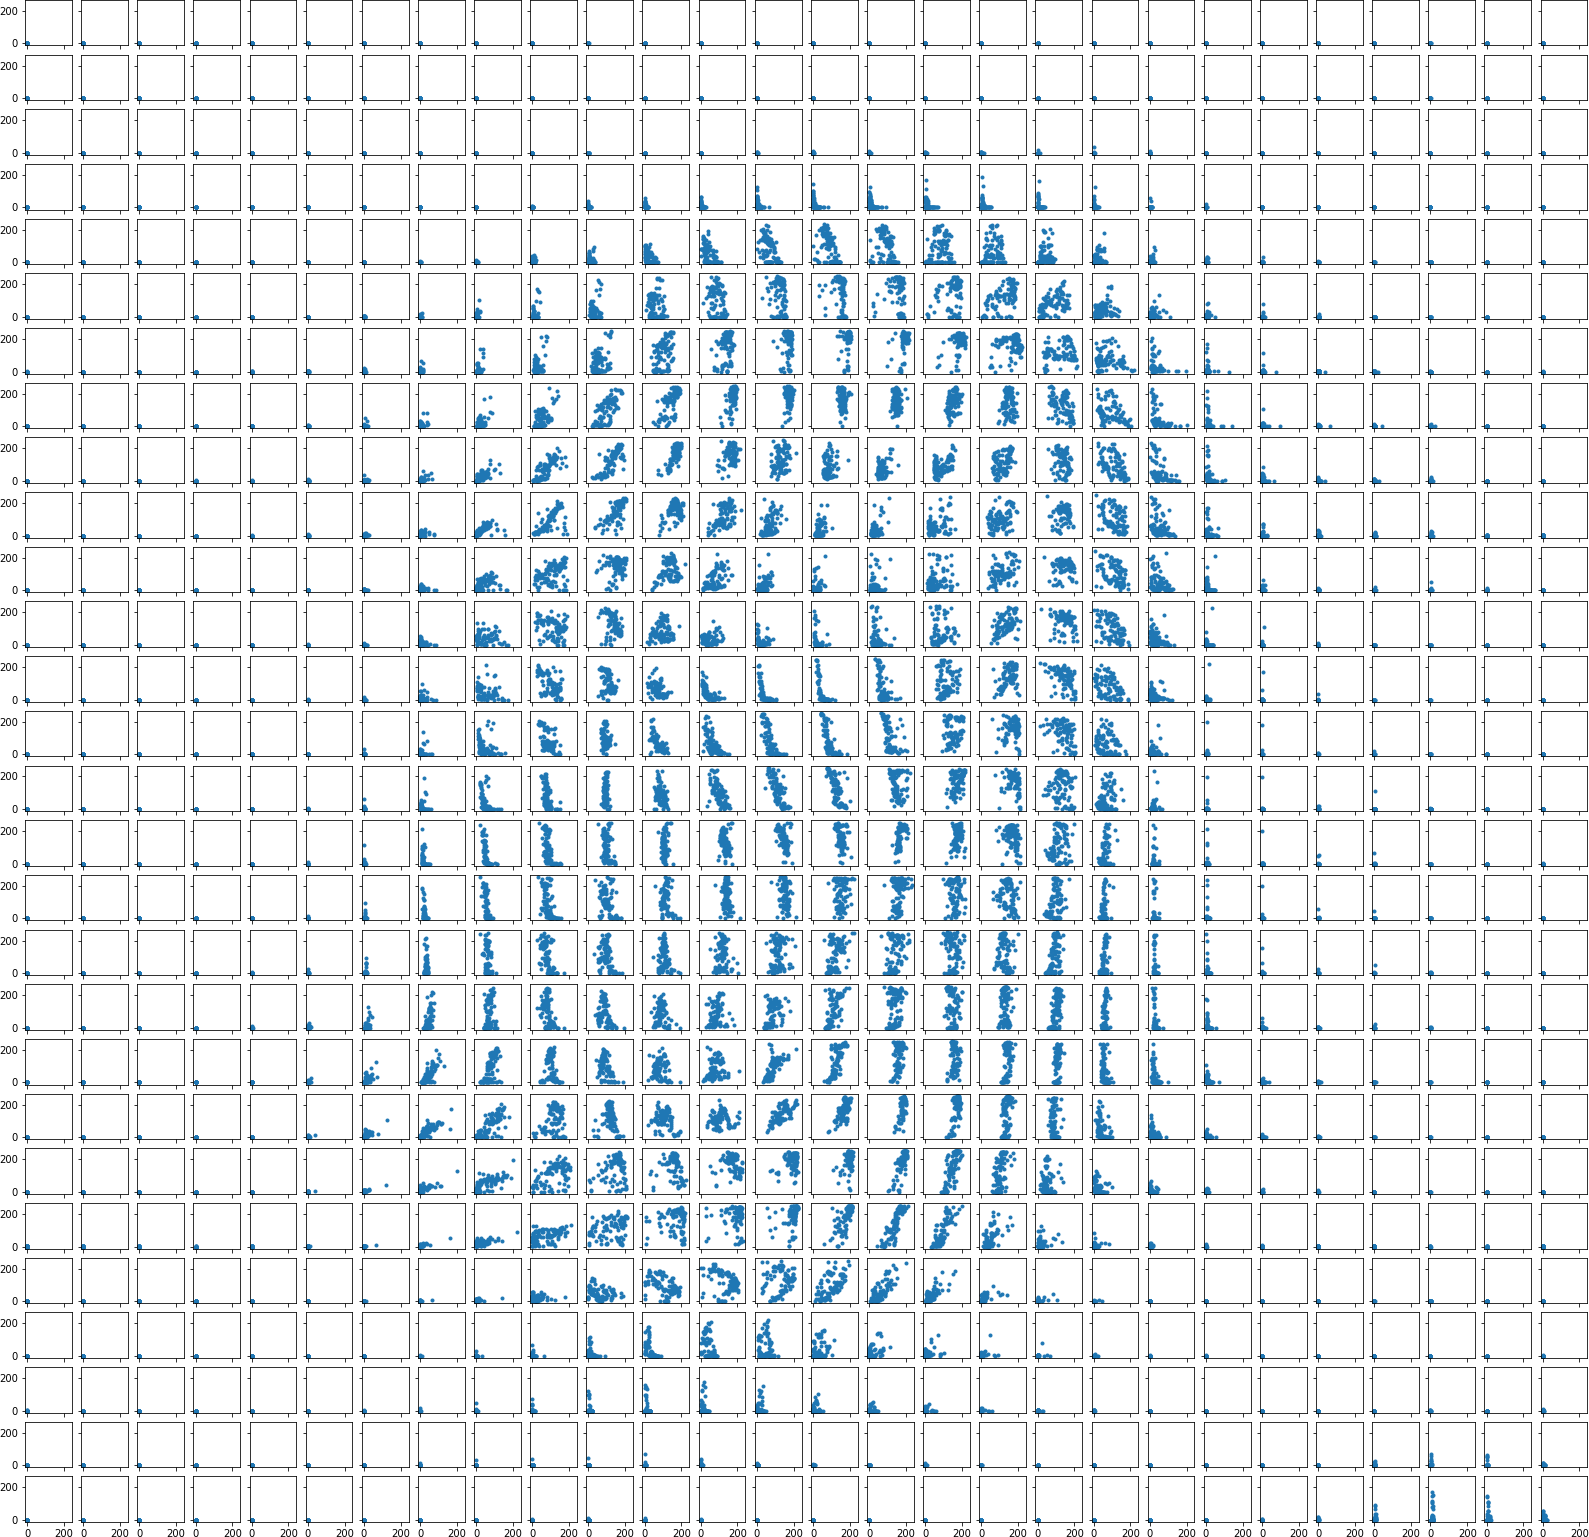
\includegraphics[width=\textwidth]{images/notprop/mnist/vlae_gan/ccs_1_2_vlae_gan.png}
\caption{Proportionality of pixel intensities when fixing $\bm{z}_2 = \bm{z}_3=\varphi$ for \ac{VLAE}-\ac{GAN} on \textsc{Mnist}. Created accordingly to Figure~\ref{fig:notprop}.}
\end{figure}


\pagebreak
\section{Additional Latent Space Embeddings (Section~\ref{subsubsec:latent_space_embeddings})}

\subsection{\textsc{Mnist}}

\begin{figure}[H]
\centering
\begin{subfigure}{.32\textwidth}
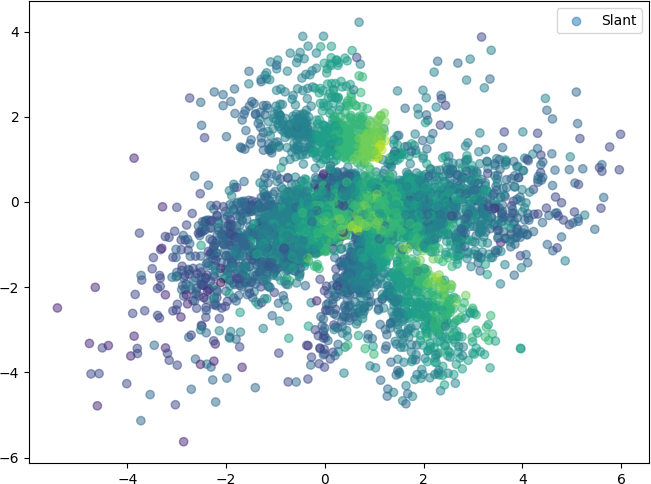
\includegraphics[width=\textwidth]{images/latent_spaces/mnist/vae_gan/embeddings_mu_0.png}
\caption{Latent space colored by digit slant}
\label{subfig:vae_mnist_latent_space_slant}
\end{subfigure}
\hfill
\begin{subfigure}{.32\textwidth}
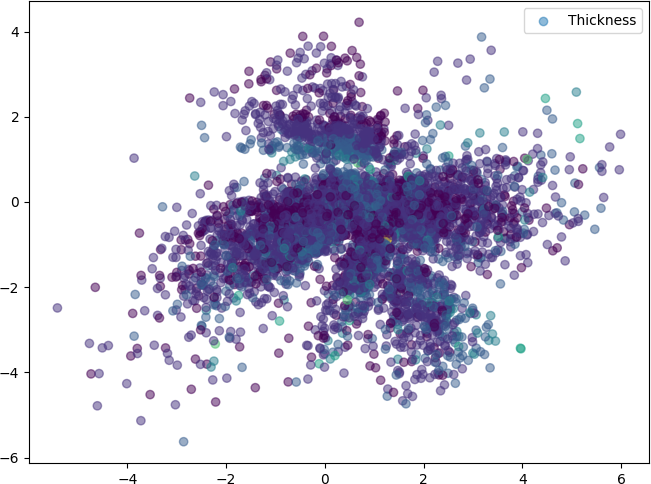
\includegraphics[width=\textwidth]{images/latent_spaces/mnist/vae_gan/embeddings_mu_1.png}
\caption{Latent space colored by digit thickness}
\label{subfig:vae_mnist_latent_space_thickness}
\end{subfigure}
\hfill
\begin{subfigure}{.32\textwidth}
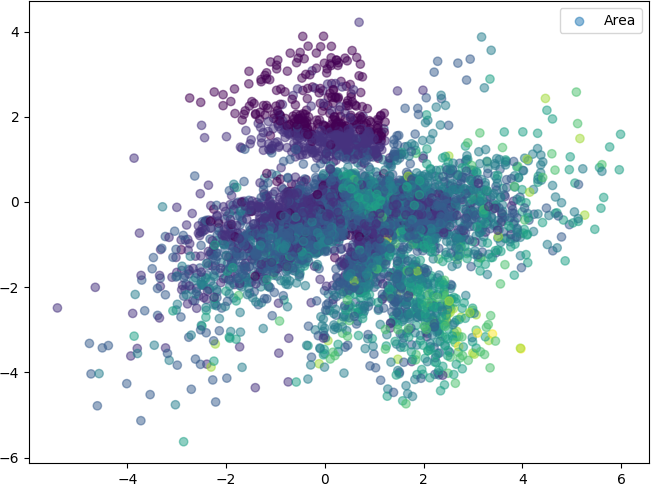
\includegraphics[width=\textwidth]{images/latent_spaces/mnist/vae_gan/embeddings_mu_2.png}
\caption{Latent space colored by digit area}
\label{subfig:vae_mnist_latent_space_area}
\end{subfigure}
\hfill
\begin{subfigure}{.24\textwidth}
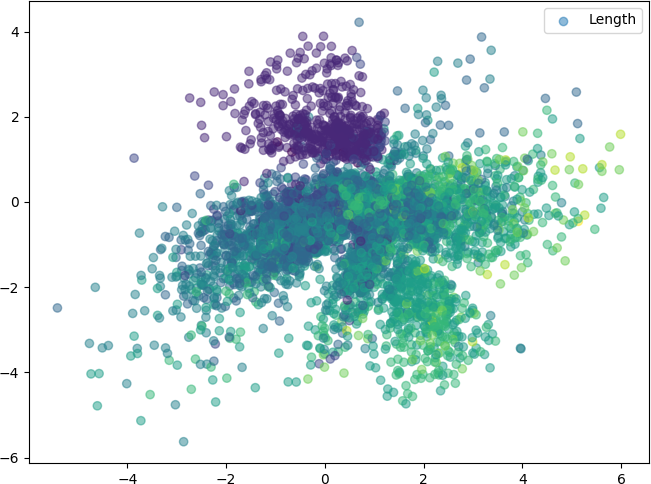
\includegraphics[width=\textwidth]{images/latent_spaces/mnist/vae_gan/embeddings_mu_3.png}
\caption{Latent space colored by digit length}
\label{subfig:vae_mnist_latent_space_length}
\end{subfigure}
\hfill
\begin{subfigure}{.24\textwidth}
\includegraphics[width=\textwidth]{images/latent_spaces/mnist/vae_gan/embeddings_mu_4.png}
\caption{Latent space colored by digit width}
\label{subfig:vae_mnist_latent_space_width}
\end{subfigure}
\hfill
\begin{subfigure}{.24\textwidth}
\includegraphics[width=\textwidth]{images/latent_spaces/mnist/vae_gan/embeddings_mu_5.png}
\caption{Latent space colored by digit height}
\label{subfig:vae_mnist_latent_space_height}
\end{subfigure}
\hfill
\begin{subfigure}{.24\textwidth}
\includegraphics[width=\textwidth]{images/latent_spaces/mnist/vae_gan/embeddings_mu_6.png}
\caption{Latent space colored by digit identity}
\label{subfig:vae_mnist_latent_space_identity}
\end{subfigure}
\caption{Latent space colored by different means of \ac{VAE}-\ac{GAN} with $dim_z=2$ trained on \textsc{Mnist} dataset}
\label{fig:vae_latent_space_mnist}
\end{figure}

\begin{landscape}
\begin{figure}[H]
\centering
\foreach \i in {1,2,3}{
\begin{subfigure}{.16\textwidth}
\includegraphics[width=\textwidth]{images/latent_spaces/mnist/vlae_gan/embeddings_mu_\i_0.png}
\caption{$z_{\i}$: digit slant}
\label{subfig:vlae_mnist_latent_space_z_\i_slant}
\end{subfigure}
\hfill
\begin{subfigure}{.16\textwidth}
\includegraphics[width=\textwidth]{images/latent_spaces/mnist/vlae_gan/embeddings_mu_\i_1.png}
\caption{$z_{\i}$: digit thickness}
\label{subfig:vlae_mnist_latent_space_z_\i_thickness}
\end{subfigure}
\hfill
\begin{subfigure}{.16\textwidth}
\includegraphics[width=\textwidth]{images/latent_spaces/mnist/vlae_gan/embeddings_mu_\i_2.png}
\caption{$z_{\i}$: digit area}
\label{subfig:vlae_mnist_latent_space_z_\i_area}
\end{subfigure}
\hfill
\begin{subfigure}{.16\textwidth}
\includegraphics[width=\textwidth]{images/latent_spaces/mnist/vlae_gan/embeddings_mu_\i_3.png}
\caption{$z_{\i}$: digit length}
\label{subfig:vlae_mnist_latent_space_z_\i_length}
\end{subfigure}
\hfill
\begin{subfigure}{.16\textwidth}
\includegraphics[width=\textwidth]{images/latent_spaces/mnist/vlae_gan/embeddings_mu_\i_4.png}
\caption{$z_{\i}$: digit width}
\label{subfig:vlae_mnist_latent_space_z_\i_width}
\end{subfigure}
\hfill
\begin{subfigure}{.16\textwidth}
\includegraphics[width=\textwidth]{images/latent_spaces/mnist/vlae_gan/embeddings_mu_\i_5.png}
\caption{$z_{\i}$: digit height}
\label{subfig:vlae_mnist_latent_space_z_\i_height}
\end{subfigure}
\hfill
\begin{subfigure}{.16\textwidth}
\includegraphics[width=\textwidth]{images/latent_spaces/mnist/vlae_gan/embeddings_mu_\i_6.png}
\caption{$z_{\i}$: digit identity}
\label{subfig:vlae_mnist_latent_space_z_\i_identity}
\end{subfigure}}
\caption{Latent space colored by different means of \ac{VLAE}-\ac{GAN} with $dim_z=2$ trained on \textsc{Mnist} dataset}
\label{fig:vlae_latent_space_mnist}
\end{figure}
\end{landscape}

\subsection{dsprites}
\begin{figure}[H]
\centering
\begin{subfigure}{.19\textwidth}
\includegraphics[width=\textwidth]{images/latent_spaces/dsprites/vae_gan/embeddings_mu_0.png}
\caption{Latent space colored by object shape}
\end{subfigure}
\hfill
\begin{subfigure}{.19\textwidth}
\includegraphics[width=\textwidth]{images/latent_spaces/dsprites/vae_gan/embeddings_mu_1.png}
\caption{Latent space colored by object scale}
\label{subfig:vae_embedding_dsprites_scale}
\end{subfigure}
\hfill
\begin{subfigure}{.19\textwidth}
\includegraphics[width=\textwidth]{images/latent_spaces/dsprites/vae_gan/embeddings_mu_2.png}
\caption{Latent space colored by object orientation}
\label{subfig:vae_embedding_dsprites_orientation}
\end{subfigure}
\hfill
\begin{subfigure}{.19\textwidth}
\includegraphics[width=\textwidth]{images/latent_spaces/dsprites/vae_gan/embeddings_mu_3.png}
\caption{Latent space colored by object $x$-position}
\end{subfigure}
\hfill
\begin{subfigure}{.19\textwidth}
\includegraphics[width=\textwidth]{images/latent_spaces/dsprites/vae_gan/embeddings_mu_4.png}
\caption{Latent space colored by object $y$-position}
\end{subfigure}
\caption{t-SNE latent space embeddings colored by different means of \ac{VAE}-\ac{GAN} with $dim_z=6$ trained on dsprites dataset}
\label{fig:vae_gan_latent_space_dsprites}
\end{figure}

\textbf{TODO: VLAE-GAN}


\pagebreak
\begin{landscape}
\section{\ac{VLAE} Networks used in Experiments on Sparsity (Section~\label{subsec:effective-network-capacity})}\label{sec:listings_sparsity_networks}
\begin{lstlisting}[caption={\textsc{Mnist}-\ac{VLAE}-factor-1 Encoder},captionpos=b,basicstyle=\tiny, label={lst:sparsity-vlae-encoder-28-fm1}]
__________________________________________________________________________________________________
Layer (type)                    Output Shape         Param #     Connected to
==================================================================================================
input_1 (InputLayer)            (None, 28, 28, 1)    0
__________________________________________________________________________________________________
inference_0_conv2d_0 (Conv2D)   (None, 14, 14, 64)   1664        input_1[0][0]
__________________________________________________________________________________________________
inference_0_relu_0 (ReLU)       (None, 14, 14, 64)   0           inference_0_conv2d_0[0][0]
__________________________________________________________________________________________________
inference_1_conv2d_0 (Conv2D)   (None, 7, 7, 64)     36928       inference_0_relu_0[0][0]
__________________________________________________________________________________________________
inference_1_relu_0 (ReLU)       (None, 7, 7, 64)     0           inference_1_conv2d_0[0][0]
__________________________________________________________________________________________________
ladder_2_conv2d_0 (Conv2D)      (None, 7, 7, 64)     36928       inference_1_relu_0[0][0]
__________________________________________________________________________________________________
ladder_2_relu_0 (ReLU)          (None, 7, 7, 64)     0           ladder_2_conv2d_0[0][0]
__________________________________________________________________________________________________
ladder_0_conv2d_0 (Conv2D)      (None, 14, 14, 64)   1664        input_1[0][0]
__________________________________________________________________________________________________
ladder_1_conv2d_0 (Conv2D)      (None, 7, 7, 64)     102464      inference_0_relu_0[0][0]
__________________________________________________________________________________________________
ladder_2_conv2d_1 (Conv2D)      (None, 7, 7, 64)     36928       ladder_2_relu_0[0][0]
__________________________________________________________________________________________________
ladder_0_relu_0 (ReLU)          (None, 14, 14, 64)   0           ladder_0_conv2d_0[0][0]
__________________________________________________________________________________________________
ladder_1_relu_0 (ReLU)          (None, 7, 7, 64)     0           ladder_1_conv2d_0[0][0]
__________________________________________________________________________________________________
ladder_2_relu_1 (ReLU)          (None, 7, 7, 64)     0           ladder_2_conv2d_1[0][0]
__________________________________________________________________________________________________
ladder_0_flatten (Flatten)      (None, 12544)        0           ladder_0_relu_0[0][0]
__________________________________________________________________________________________________
ladder_1_flatten (Flatten)      (None, 3136)         0           ladder_1_relu_0[0][0]
__________________________________________________________________________________________________
ladder_2_flatten (Flatten)      (None, 3136)         0           ladder_2_relu_1[0][0]
__________________________________________________________________________________________________
mu_1 (Dense)                    (None, 2)            25090       ladder_0_flatten[0][0]
__________________________________________________________________________________________________
log_var_1 (Dense)               (None, 2)            25090       ladder_0_flatten[0][0]
__________________________________________________________________________________________________
mu_2 (Dense)                    (None, 2)            6274        ladder_1_flatten[0][0]
__________________________________________________________________________________________________
log_var_2 (Dense)               (None, 2)            6274        ladder_1_flatten[0][0]
__________________________________________________________________________________________________
mu_3 (Dense)                    (None, 2)            6274        ladder_2_flatten[0][0]
__________________________________________________________________________________________________
log_var_3 (Dense)               (None, 2)            6274        ladder_2_flatten[0][0]
__________________________________________________________________________________________________
z_1_latent (Lambda)             (None, 2)            0           mu_1[0][0]
log_var_1[0][0]
__________________________________________________________________________________________________
z_2_latent (Lambda)             (None, 2)            0           mu_2[0][0]
log_var_2[0][0]
__________________________________________________________________________________________________
z_3_latent (Lambda)             (None, 2)            0           mu_3[0][0]
log_var_3[0][0]
==================================================================================================
Total params: 291,852
Trainable params: 291,852
Non-trainable params: 0
__________________________________________________________________________________________________
\end{lstlisting}
\pagebreak
\begin{lstlisting}[caption={Initial \ac{VLAE} network decoder used for network sparsity experiments},captionpos=b,basicstyle=\tiny, label={lst:sparsity-vlae-decoder-28-fm1}]
__________________________________________________________________________________________________
Layer (type)                    Output Shape         Param #     Connected to
==================================================================================================
z_3 (InputLayer)                (None, 2)            0
__________________________________________________________________________________________________
generative_2_dense_0 (Dense)    (None, 1024)         3072        z_3[0][0]
__________________________________________________________________________________________________
generative_2_relu_0 (ReLU)      (None, 1024)         0           generative_2_dense_0[0][0]
__________________________________________________________________________________________________
generative_2_dense_1 (Dense)    (None, 1024)         1049600     generative_2_relu_0[0][0]
__________________________________________________________________________________________________
generative_2_relu_1 (ReLU)      (None, 1024)         0           generative_2_dense_1[0][0]
__________________________________________________________________________________________________
z_2 (InputLayer)                (None, 2)            0
__________________________________________________________________________________________________
concatenate_2_and_1 (Concatenat (None, 1026)         0           generative_2_relu_1[0][0]
z_2[0][0]
__________________________________________________________________________________________________
generative_1_dense_0 (Dense)    (None, 1024)         1051648     concatenate_2_and_1[0][0]
__________________________________________________________________________________________________
generative_1_relu_0 (ReLU)      (None, 1024)         0           generative_1_dense_0[0][0]
__________________________________________________________________________________________________
generative_1_dense_1 (Dense)    (None, 1024)         1049600     generative_1_relu_0[0][0]
__________________________________________________________________________________________________
generative_1_relu_1 (ReLU)      (None, 1024)         0           generative_1_dense_1[0][0]
__________________________________________________________________________________________________
z_1 (InputLayer)                (None, 2)            0
__________________________________________________________________________________________________
concatenate_1_and_0 (Concatenat (None, 1026)         0           generative_1_relu_1[0][0]
z_1[0][0]
__________________________________________________________________________________________________
generative_0_dense_0 (Dense)    (None, 3136)         3220672     concatenate_1_and_0[0][0]
__________________________________________________________________________________________________
generative_0_relu_0 (ReLU)      (None, 3136)         0           generative_0_dense_0[0][0]
__________________________________________________________________________________________________
generative_0_reshape_0 (Reshape (None, 7, 7, 64)     0           generative_0_relu_0[0][0]
__________________________________________________________________________________________________
generative_0_conv2d_transpose_0 (None, 14, 14, 64)   102464      generative_0_reshape_0[0][0]
__________________________________________________________________________________________________
generative_0_leaky_relu_transpo (None, 14, 14, 64)   0           generative_0_conv2d_transpose_0[0
__________________________________________________________________________________________________
generative_0_conv2d_transpose_1 (None, 28, 28, 64)   36928       generative_0_leaky_relu_transpose
__________________________________________________________________________________________________
generative_0_leaky_relu_transpo (None, 28, 28, 64)   0           generative_0_conv2d_transpose_1[0
__________________________________________________________________________________________________
generative_0_conv2d_transpose_2 (None, 28, 28, 1)    1601        generative_0_leaky_relu_transpose
__________________________________________________________________________________________________
generative_0_sigmoid_0 (Activat (None, 28, 28, 1)    0           generative_0_conv2d_transpose_2[0
==================================================================================================
Total params: 6,515,585
Trainable params: 6,515,585
Non-trainable params: 0
__________________________________________________________________________________________________
\end{lstlisting}
\pagebreak
\begin{lstlisting}[caption={\textsc{Mnist}-\ac{VLAE}-factor-2 Encoder},captionpos=b,basicstyle=\tiny, label={lst:sparsity-vlae-encoder-28-fm2}]
__________________________________________________________________________________________________
Layer (type)                    Output Shape         Param #     Connected to
==================================================================================================
input_1 (InputLayer)            (None, 28, 28, 1)    0
__________________________________________________________________________________________________
inference_0_conv2d_0 (Conv2D)   (None, 14, 14, 32)   832         input_1[0][0]
__________________________________________________________________________________________________
inference_0_relu_0 (ReLU)       (None, 14, 14, 32)   0           inference_0_conv2d_0[0][0]
__________________________________________________________________________________________________
inference_1_conv2d_0 (Conv2D)   (None, 7, 7, 32)     9248        inference_0_relu_0[0][0]
__________________________________________________________________________________________________
inference_1_relu_0 (ReLU)       (None, 7, 7, 32)     0           inference_1_conv2d_0[0][0]
__________________________________________________________________________________________________
ladder_2_conv2d_0 (Conv2D)      (None, 7, 7, 32)     9248        inference_1_relu_0[0][0]
__________________________________________________________________________________________________
ladder_2_relu_0 (ReLU)          (None, 7, 7, 32)     0           ladder_2_conv2d_0[0][0]
__________________________________________________________________________________________________
ladder_0_conv2d_0 (Conv2D)      (None, 14, 14, 32)   832         input_1[0][0]
__________________________________________________________________________________________________
ladder_1_conv2d_0 (Conv2D)      (None, 7, 7, 32)     25632       inference_0_relu_0[0][0]
__________________________________________________________________________________________________
ladder_2_conv2d_1 (Conv2D)      (None, 7, 7, 32)     9248        ladder_2_relu_0[0][0]
__________________________________________________________________________________________________
ladder_0_relu_0 (ReLU)          (None, 14, 14, 32)   0           ladder_0_conv2d_0[0][0]
__________________________________________________________________________________________________
ladder_1_relu_0 (ReLU)          (None, 7, 7, 32)     0           ladder_1_conv2d_0[0][0]
__________________________________________________________________________________________________
ladder_2_relu_1 (ReLU)          (None, 7, 7, 32)     0           ladder_2_conv2d_1[0][0]
__________________________________________________________________________________________________
ladder_0_flatten (Flatten)      (None, 6272)         0           ladder_0_relu_0[0][0]
__________________________________________________________________________________________________
ladder_1_flatten (Flatten)      (None, 1568)         0           ladder_1_relu_0[0][0]
__________________________________________________________________________________________________
ladder_2_flatten (Flatten)      (None, 1568)         0           ladder_2_relu_1[0][0]
__________________________________________________________________________________________________
mu_1 (Dense)                    (None, 2)            12546       ladder_0_flatten[0][0]
__________________________________________________________________________________________________
log_var_1 (Dense)               (None, 2)            12546       ladder_0_flatten[0][0]
__________________________________________________________________________________________________
mu_2 (Dense)                    (None, 2)            3138        ladder_1_flatten[0][0]
__________________________________________________________________________________________________
log_var_2 (Dense)               (None, 2)            3138        ladder_1_flatten[0][0]
__________________________________________________________________________________________________
mu_3 (Dense)                    (None, 2)            3138        ladder_2_flatten[0][0]
__________________________________________________________________________________________________
log_var_3 (Dense)               (None, 2)            3138        ladder_2_flatten[0][0]
__________________________________________________________________________________________________
z_1_latent (Lambda)             (None, 2)            0           mu_1[0][0]
log_var_1[0][0]
__________________________________________________________________________________________________
z_2_latent (Lambda)             (None, 2)            0           mu_2[0][0]
log_var_2[0][0]
__________________________________________________________________________________________________
z_3_latent (Lambda)             (None, 2)            0           mu_3[0][0]
log_var_3[0][0]
==================================================================================================
Total params: 92,684
Trainable params: 92,684
Non-trainable params: 0
__________________________________________________________________________________________________
\end{lstlisting}
\pagebreak
\begin{lstlisting}[caption={\ac{VLAE} network decoder used for network sparsity experiments with half the number of feature maps},captionpos=b,basicstyle=\tiny, label={lst:sparsity-vlae-decoder-28-fm2}]
__________________________________________________________________________________________________
Layer (type)                    Output Shape         Param #     Connected to
==================================================================================================
z_3 (InputLayer)                (None, 2)            0
__________________________________________________________________________________________________
generative_2_dense_0 (Dense)    (None, 512)          1536        z_3[0][0]
__________________________________________________________________________________________________
generative_2_relu_0 (ReLU)      (None, 512)          0           generative_2_dense_0[0][0]
__________________________________________________________________________________________________
generative_2_dense_1 (Dense)    (None, 512)          262656      generative_2_relu_0[0][0]
__________________________________________________________________________________________________
generative_2_relu_1 (ReLU)      (None, 512)          0           generative_2_dense_1[0][0]
__________________________________________________________________________________________________
z_2 (InputLayer)                (None, 2)            0
__________________________________________________________________________________________________
concatenate_2_and_1 (Concatenat (None, 514)          0           generative_2_relu_1[0][0]
z_2[0][0]
__________________________________________________________________________________________________
generative_1_dense_0 (Dense)    (None, 512)          263680      concatenate_2_and_1[0][0]
__________________________________________________________________________________________________
generative_1_relu_0 (ReLU)      (None, 512)          0           generative_1_dense_0[0][0]
__________________________________________________________________________________________________
generative_1_dense_1 (Dense)    (None, 512)          262656      generative_1_relu_0[0][0]
__________________________________________________________________________________________________
generative_1_relu_1 (ReLU)      (None, 512)          0           generative_1_dense_1[0][0]
__________________________________________________________________________________________________
z_1 (InputLayer)                (None, 2)            0
__________________________________________________________________________________________________
concatenate_1_and_0 (Concatenat (None, 514)          0           generative_1_relu_1[0][0]
z_1[0][0]
__________________________________________________________________________________________________
generative_0_dense_0 (Dense)    (None, 1568)         807520      concatenate_1_and_0[0][0]
__________________________________________________________________________________________________
generative_0_relu_0 (ReLU)      (None, 1568)         0           generative_0_dense_0[0][0]
__________________________________________________________________________________________________
generative_0_reshape_0 (Reshape (None, 7, 7, 32)     0           generative_0_relu_0[0][0]
__________________________________________________________________________________________________
generative_0_conv2d_transpose_0 (None, 14, 14, 32)   25632       generative_0_reshape_0[0][0]
__________________________________________________________________________________________________
generative_0_leaky_relu_transpo (None, 14, 14, 32)   0           generative_0_conv2d_transpose_0[0
__________________________________________________________________________________________________
generative_0_conv2d_transpose_1 (None, 28, 28, 32)   9248        generative_0_leaky_relu_transpose
__________________________________________________________________________________________________
generative_0_leaky_relu_transpo (None, 28, 28, 32)   0           generative_0_conv2d_transpose_1[0
__________________________________________________________________________________________________
generative_0_conv2d_transpose_2 (None, 28, 28, 1)    801         generative_0_leaky_relu_transpose
__________________________________________________________________________________________________
generative_0_sigmoid_0 (Activat (None, 28, 28, 1)    0           generative_0_conv2d_transpose_2[0
==================================================================================================
Total params: 1,633,729
Trainable params: 1,633,729
Non-trainable params: 0
__________________________________________________________________________________________________
\end{lstlisting}
\pagebreak
\begin{lstlisting}[caption={\ac{VLAE} network encoder used for network sparsity experiments with one third the number of feature maps},captionpos=b,basicstyle=\tiny, label={lst:sparsity-vlae-encoder-28-fm3}]
__________________________________________________________________________________________________
Layer (type)                    Output Shape         Param #     Connected to
==================================================================================================
input_1 (InputLayer)            (None, 28, 28, 1)    0
__________________________________________________________________________________________________
inference_0_conv2d_0 (Conv2D)   (None, 14, 14, 22)   572         input_1[0][0]
__________________________________________________________________________________________________
inference_0_relu_0 (ReLU)       (None, 14, 14, 22)   0           inference_0_conv2d_0[0][0]
__________________________________________________________________________________________________
inference_1_conv2d_0 (Conv2D)   (None, 7, 7, 22)     4378        inference_0_relu_0[0][0]
__________________________________________________________________________________________________
inference_1_relu_0 (ReLU)       (None, 7, 7, 22)     0           inference_1_conv2d_0[0][0]
__________________________________________________________________________________________________
ladder_2_conv2d_0 (Conv2D)      (None, 7, 7, 22)     4378        inference_1_relu_0[0][0]
__________________________________________________________________________________________________
ladder_2_relu_0 (ReLU)          (None, 7, 7, 22)     0           ladder_2_conv2d_0[0][0]
__________________________________________________________________________________________________
ladder_0_conv2d_0 (Conv2D)      (None, 14, 14, 22)   572         input_1[0][0]
__________________________________________________________________________________________________
ladder_1_conv2d_0 (Conv2D)      (None, 7, 7, 22)     12122       inference_0_relu_0[0][0]
__________________________________________________________________________________________________
ladder_2_conv2d_1 (Conv2D)      (None, 7, 7, 22)     4378        ladder_2_relu_0[0][0]
__________________________________________________________________________________________________
ladder_0_relu_0 (ReLU)          (None, 14, 14, 22)   0           ladder_0_conv2d_0[0][0]
__________________________________________________________________________________________________
ladder_1_relu_0 (ReLU)          (None, 7, 7, 22)     0           ladder_1_conv2d_0[0][0]
__________________________________________________________________________________________________
ladder_2_relu_1 (ReLU)          (None, 7, 7, 22)     0           ladder_2_conv2d_1[0][0]
__________________________________________________________________________________________________
ladder_0_flatten (Flatten)      (None, 4312)         0           ladder_0_relu_0[0][0]
__________________________________________________________________________________________________
ladder_1_flatten (Flatten)      (None, 1078)         0           ladder_1_relu_0[0][0]
__________________________________________________________________________________________________
ladder_2_flatten (Flatten)      (None, 1078)         0           ladder_2_relu_1[0][0]
__________________________________________________________________________________________________
mu_1 (Dense)                    (None, 2)            8626        ladder_0_flatten[0][0]
__________________________________________________________________________________________________
log_var_1 (Dense)               (None, 2)            8626        ladder_0_flatten[0][0]
__________________________________________________________________________________________________
mu_2 (Dense)                    (None, 2)            2158        ladder_1_flatten[0][0]
__________________________________________________________________________________________________
log_var_2 (Dense)               (None, 2)            2158        ladder_1_flatten[0][0]
__________________________________________________________________________________________________
mu_3 (Dense)                    (None, 2)            2158        ladder_2_flatten[0][0]
__________________________________________________________________________________________________
log_var_3 (Dense)               (None, 2)            2158        ladder_2_flatten[0][0]
__________________________________________________________________________________________________
z_1_latent (Lambda)             (None, 2)            0           mu_1[0][0]
log_var_1[0][0]
__________________________________________________________________________________________________
z_2_latent (Lambda)             (None, 2)            0           mu_2[0][0]
log_var_2[0][0]
__________________________________________________________________________________________________
z_3_latent (Lambda)             (None, 2)            0           mu_3[0][0]
log_var_3[0][0]
==================================================================================================
Total params: 52,284
Trainable params: 52,284
Non-trainable params: 0
__________________________________________________________________________________________________
\end{lstlisting}
\pagebreak
\begin{lstlisting}[caption={\textsc{Mnist}-\ac{VLAE}-factor-3 Decoder},captionpos=b,basicstyle=\tiny, label={lst:sparsity-vlae-decoder-28-fm3}]
__________________________________________________________________________________________________
Layer (type)                    Output Shape         Param #     Connected to
==================================================================================================
z_3 (InputLayer)                (None, 2)            0
__________________________________________________________________________________________________
generative_2_dense_0 (Dense)    (None, 342)          1026        z_3[0][0]
__________________________________________________________________________________________________
generative_2_relu_0 (ReLU)      (None, 342)          0           generative_2_dense_0[0][0]
__________________________________________________________________________________________________
generative_2_dense_1 (Dense)    (None, 342)          117306      generative_2_relu_0[0][0]
__________________________________________________________________________________________________
generative_2_relu_1 (ReLU)      (None, 342)          0           generative_2_dense_1[0][0]
__________________________________________________________________________________________________
z_2 (InputLayer)                (None, 2)            0
__________________________________________________________________________________________________
concatenate_2_and_1 (Concatenat (None, 344)          0           generative_2_relu_1[0][0]
z_2[0][0]
__________________________________________________________________________________________________
generative_1_dense_0 (Dense)    (None, 342)          117990      concatenate_2_and_1[0][0]
__________________________________________________________________________________________________
generative_1_relu_0 (ReLU)      (None, 342)          0           generative_1_dense_0[0][0]
__________________________________________________________________________________________________
generative_1_dense_1 (Dense)    (None, 342)          117306      generative_1_relu_0[0][0]
__________________________________________________________________________________________________
generative_1_relu_1 (ReLU)      (None, 342)          0           generative_1_dense_1[0][0]
__________________________________________________________________________________________________
z_1 (InputLayer)                (None, 2)            0
__________________________________________________________________________________________________
concatenate_1_and_0 (Concatenat (None, 344)          0           generative_1_relu_1[0][0]
z_1[0][0]
__________________________________________________________________________________________________
generative_0_dense_0 (Dense)    (None, 1078)         371910      concatenate_1_and_0[0][0]
__________________________________________________________________________________________________
generative_0_relu_0 (ReLU)      (None, 1078)         0           generative_0_dense_0[0][0]
__________________________________________________________________________________________________
generative_0_reshape_0 (Reshape (None, 7, 7, 22)     0           generative_0_relu_0[0][0]
__________________________________________________________________________________________________
generative_0_conv2d_transpose_0 (None, 14, 14, 22)   12122       generative_0_reshape_0[0][0]
__________________________________________________________________________________________________
generative_0_leaky_relu_transpo (None, 14, 14, 22)   0           generative_0_conv2d_transpose_0[0
__________________________________________________________________________________________________
generative_0_conv2d_transpose_1 (None, 28, 28, 22)   4378        generative_0_leaky_relu_transpose
__________________________________________________________________________________________________
generative_0_leaky_relu_transpo (None, 28, 28, 22)   0           generative_0_conv2d_transpose_1[0
__________________________________________________________________________________________________
generative_0_conv2d_transpose_2 (None, 28, 28, 1)    551         generative_0_leaky_relu_transpose
__________________________________________________________________________________________________
generative_0_sigmoid_0 (Activat (None, 28, 28, 1)    0           generative_0_conv2d_transpose_2[0
==================================================================================================
Total params: 742,589
Trainable params: 742,589
Non-trainable params: 0
__________________________________________________________________________________________________
\end{lstlisting}
\end{landscape}

\pagebreak

\section{Discriminator Network used in Section \ref{subsec:vae-generated-samples-vs-true-samples}}\label{sec:listing_discriminator_network}
\begin{lstlisting}[caption={The discriminator network used to distinguish generated \ac{VAE}/\ac{VLAE} samples from true \textsc{MNIST} images.},captionpos=b]
_________________________________________________________________
Layer (type)                 Output Shape Param #
=================================================================
input_2 (InputLayer)         (None, 28, 28, 1)         0
_________________________________________________________________
conv2d_4 (Conv2D)            (None, 24, 24, 20)        520
_________________________________________________________________
leaky_re_lu_4 (LeakyReLU)    (None, 24, 24, 20)        0
_________________________________________________________________
batch_normalization_23 (Batc (None, 24, 24, 20)        80
_________________________________________________________________
conv2d_5 (Conv2D)            (None, 22, 22, 20)        3620
_________________________________________________________________
leaky_re_lu_5 (LeakyReLU)    (None, 22, 22, 20)        0
_________________________________________________________________
batch_normalization_24 (Batc (None, 22, 22, 20)        80
_________________________________________________________________
flatten_5 (Flatten)          (None, 9680)              0
_________________________________________________________________
dense_15 (Dense)             (None, 100)               968100
_________________________________________________________________
leaky_re_lu_6 (LeakyReLU)    (None, 100)               0
_________________________________________________________________
batch_normalization_25 (Batc (None, 100)               400
_________________________________________________________________
dense_16 (Dense)             (None, 1)                 101
=================================================================
Total params: 972,901
Trainable params: 972,621
Non-trainable params: 280
_________________________________________________________________
\end{lstlisting}


\newpage
\section*{Acronyms}
\begin{acronym}[TDMA]
\acro{AdaIN}{Adaptive Instance Normalization}
\acro{ALAE}{Adversarial Latent Autoencoder}
\acro{VAE}{Variational Autoencoder}
\acro{CNN}{Convolutional Neural Network}
\acro{IT}{Inferior Temporal Cortex}
\acro{ReLU}{Rectified Linear Unit}
\acro{LeakyReLU}{Leaky Rectified Linear Unit}
\acro{ILSVRC2017}{Large Scale Visual Recognition Challenge 2017}
\acro{MSE}{Mean Squared Error}
\acro{RDM}{Representational Dissimilarity Matrix}
\acro{KL-divergence}{Kullback-Leibler divergence}
\acro{KL}{Kullback-Leibler}
\acro{ELBO}{Evidence Lower Bound}
\acro{PDF}{Probability Density Function}
\acro{NLP}{Natural Language Processing}
\acro{GAN}{Generative Adversarial Network}
\acro{VLAE}{Variational Ladder Autoencoder}
\acro{LVAE}{Ladder Variational Autoencoder}
\acro{CNS}{Central Nervous System}
\acro{V1}{Primary Visual Cortex}
\acro{V2}{Secondary Visual Cortex}
\acro{V4}{Quaternary Visual Cortex}
\acro{LGN}{Lateral Geniculate Nucleus}
\acro{TEO}{Temporo-Occipital Area}
\end{acronym}
\newpage
\listoffigures
\newpage
\listoftables
\newpage
\section*{Erklärung}

Ich erkläre, dass das Thema dieser Arbeit nicht identisch ist mit dem Thema einer von mir bereits für eine andere Prüfung eingereichte Arbeit.\par
Ich erkläre weiterhin, dass ich die Arbeit nicht bereits an einer anderen Hochschule zur Erlangung eines akademischen Grades eingereicht habe.\par
\vspace{2cm}
Ich versichere, dass ich die Arbeit selbstständig verfasst und keine anderen als die angegebenen Quellen benutzt habe.
Die Stellen der Arbeit, die anderen Werken dem Wortlaut oder dem Sinn nach entnommen sind, habe ich unter Angabe der Quellen der Entlehnung kenntlich gemacht.
Dies gilt sinngemäß auch für gelieferte Zeichnungen, Skizzen, bildliche Darstellungen und dergleichen.

\vfill

\hspace{2cm} Ort, Datum \hfill Unterschrift \hspace{2cm}


\end{document}
